\svnkwsave{$RepoFile: siminos/spatiotemp/chapter/blogMNG18.tex $}
\svnidlong {$HeadURL: svn://zero.physics.gatech.edu/siminos/spatiotemp/chapter/blogMNG18.tex $}
{$LastChangedDate: 2020-09-06 00:05:02 -0400 (Sun, 06 Sep 2020) $}
{$LastChangedRevision: 6859 $} {$LastChangedBy: predrag $}
\svnid{$Id: blogMNG18.tex 6859 2019-05-09 20:51:31Z predrag $}

\chapter{Matt's 2018 blog}
\label{chap:blogMNG18}
% Predrag                                          15 March 2019

\begin{description}


\MNGpost{2018-01-08}{
\begin{description}
\item[initial conditions]
I believe all but one issue are ironed out now, the only problem that
still arises is when an orbit gets stuck near an equilibrium for the
entire length of time integration of a close recurrence will the initial
condition generation produce something not worthwhile.

The way that this was accomplished was by tuning the restart procedure as
well as tuning time integration in the close recurrence procedure, as
well as the total time being integrated, number of time steps. I have
abandoned the Poincar\'e hyperplane in favor of this fine time
integration. I also abandoned playing around with running a coarse time
integration and then refining it as this produced strange results. I
thought that it would merely produce a larger region around the local
minimum (region of the close recurrence plot) by tuning the amount of
time integrated of the second time integration as well as increasing the
number of time steps but sometimes this procedure would either restart in
the wrong spot or miss the local minimum returning a larger (in terms of
the residual of the $L_2$ norm of the difference between starting and
final points.) Therefore, I decided it was wrothwhile due to other
speed-ups to just perform the finer close recurrence and if nothing is
found then just restart.

\item[spatiotemp code]
In between testing these new initial conditions I have decided to rewrite
and add some different ways that the hookstep is calculated. This is due
to there being a lack of safety nets for when the hookstep code
previously would fail and the code would have to abort. This seems to be
due to trying to optimize a hookstep for too large of a trust region.
While normally you would just check the residual and then if it isn't
reduced, one would reduce the trust region and continue. But, in my case
this would lead to numerical overflow and the code would abort.
Therefore, a safer, more constrained optimization protocol had to be
adopted. Now, the parameter that computes the size of the corrections is
always bounded and if it fails to lie in these bounds, a value is chosen
based on the iteration.

In other words when asked to find a vector $\hat{s}$ that minimizes $||D
\hat{s} - \hat{b} ||_2 $ subject to $\hat{s} \leq \delta $, the general
solution is given by\rf{Dennis96,ChanKers13},
\beq \label{eqn:hookstep}
\hat{s} = \frac{\hat{b} d_i}{d_i^2 + \mu} \mbox{    (no summation)}
\,,
\eeq
\ie, this is the solution that minimizes $\Phi(\mu) = ||s(\mu)||^2 - \delta^2$.

Now I will elect to follow the procedure in \refref{Dennis96} that instills bounds on the parameter $\mu$.
The lower bound will be chosen by the ``normal"
Newton procedure instead of the one that is adapted to solve for $\mu$ for this problem.

During each iteration to update $\mu$, we calculate lower($\ell$) and upper (u) bounds by

Initializing them at first by $\ell_0 =- \frac{\Phi(0)}{\Phi^{\prime}(0)}$ and $u_0= |\nabla F(x_c)|/\delta_c$.

Then at each step for the lower bound we increase the lower bound by taking the maximum between

\beq
\ell_{+}^N = \mu_c - \frac{\Phi(\mu_c)}{\Phi^{\prime}(\mu_c)}
\eeq

and the current lower bound.

To update the upper bound we decrease it by taking the minimum between the current upper bound and the
current value of mu,
\beq
u_{+} = min(u_c , \mu_c)
\eeq

where $+$ indicates the next value of the parameters, and ``c" indicates the current value (following
\rf{Dennis96} notation as to not confuse myself).

The next iterate $\mu_{+}$ is calculated by the 'adapted' Newton method.

\beq
\mu_{+} = \mu_c - \frac{s(\mu_c)}{\delta_c} \frac{\Phi(\mu_c)}{\Phi^{\prime}(\mu_c)}
\eeq

and then tested to see if it lies in our trusted region $[\ell_{+}, u_{+}]$. If it doesn't,
then the next iterate $\mu_{+}$ is taken to be $\max ((\ell_{+} u_{+})^{1/2}, 10^{-3} u_{+})$
which Dennis and Schnable claim is most often used to calculate the initial value $\mu_0$.

We then let the iteration run until the norm of the hookstep lies in our trust region. (I might change
this to be until the residual of the function $\Phi (\mu)$ is minimized sufficiently).

After these changes, we then need to decide to do with the trust region and our current hookstep.
If the hookstep does not minimize the residual sufficiently when compared to the linear model,
we need to decrease the trust region radius (which they say they just do by halving it but also give
details on calculating a multiplier between one tenth and one half). If the residual compares
favorably to the quadratic residual then we can keep this as a backup step before increasing the
trust region radius by a factor of two and attempting to try again.

\end{description}
}

\MNGpost{2018-01-10}{
Finished the implementation of most of the changes to hookstep and initial condition generation,
whether they need any changes is up to testing
that is proceeding now.

Used new initial condition generation code to generate a few hundred guesses for spatial domains that take integer
values in the range $L \exists [22,43]$. Now I just need a little time to run code and see if anything converges
}

\begin{figure}
\begin{minipage}[height=.32\textheight]{.45\textwidth}
\centering \small{\texttt{(a)}}
\includegraphics[width=\textwidth,height=.32\textheight]{MNG_st_init2}
\end{minipage}
\\
\begin{minipage}[height=.32\textheight]{.45\textwidth}
\centering \small{\texttt{(b)}}
\includegraphics[width=\textwidth,height=.32\textheight]{MNG_st_adj2}
\end{minipage}
\begin{minipage}[height=.32\textheight]{.45\textwidth}
\centering \small{\texttt{(c)}}
\includegraphics[width=\textwidth,height=.32\textheight]{MNG_st_f2}
\end{minipage}
\caption{ \label{fig:MNG2}
(a) Initial spatiotemporal initial condition, whose dimensions are
$(\speriod{},\period{})=(22.0,103.125)$.
(b) Approximate spatiotemporal fixed point after adjoint descent,
$(\speriod{},\period{})=(22.026,103.13)$.
(c) Converged spatiotemporal fixed point after hybrid method,
$(\speriod{},\period{})=(22.232,102.94)$.
}
\end{figure}


\MNGpost{2018-01-12}{
\begin{description}
\item[{\twots}]

Fixed errors in the blog. Uploaded Figures, now to expand on them.

The first set of figures \reffig{fig:MNG-vndst} is an example of using variational Newton descent in time to
improve an arbitrarily poor initial condition such that it converges under application of my spatiotemporal fixed
point code after the Newton Descent.

The second set of figures in \reffig{fig:MNG2} is an example of convergence without using any modfication beforehand
via Newton Descent. The solution was converges to within machine precision by using a hybrid method.
Namely, the initial condition was first run through Mohammad's adjoint descent and then once a certain number
of steps had been taken (In practice this is set to a fixed number of steps but it is usually a sufficient
number to reach a region where the adjoint descent only provides marginal improvement). Secondly,
it was sent to an adaptive Newton method, that decreases the residual of the cost functional
by decreasing the step length until this is ensured. I elected to try this method because even though
I completely changed the hookstep code it still doesn't seem to be up to snuff when it comes to efficiency.

The perplexing part about the spatiotemporal fixed point in \reffig{fig:MNG2} is that while the initial condition
represents one period of a \ppo, the final, resulting spatiotemporal fixed point is seemingly
five copies of a shorter orbit (in time). As there is little difference between (b) and (c) in \reffig{fig:MNG2}
it seems this is due to the adjoint descent. It could just be an inaccurate initial condition, or perhaps the
adjoint descent is missing the longer orbit for its shadow.

\item[initial conditions]

It turns out the vast majority of initial conditions were equilibria; I instilled a lower bound that should
prevent these from being generated, but it's a very heuristic process.

\end{description}
}

\MNGpost{2018-01-16}{
\begin{description}
\item[Robust modes in hydrodynamic flows]
Read Professor Gunaratne's paper that is the focus of his planned talk here.
I was going to ask whether
partitioning simulations in space and comparing their spectra would also
be a valid or worthwhile endeavor as currently he takes a series of snapshots
of the flow in a computational cell, uses subsets to compare spectra in time.
(I believe the subsets were the full series, the first half, the second half, even
numbered snapshots and odd numbered snapshots). Dynamic mode decomposition is then performed on these
subsets and robust modes are defined by modes that are common to all subsets.

\item[spatiotemp]
Almost done with the automation procedure to find spatiotemporal fixed points associated
with \ppo s. I combined the initial condition generation code and the solution converging code
into one Python script. What it will do is work through
different domain sizes one-by-one, produce initial conditions for the convergence code, and if
the initial conditions satisfy certain requirements on the residual of the cost functional, run
the convergence code on it. Currently have it setup so that long trawls of {\statesp} are performed
as opposed to shorter more accurate trawls, getting some weird results so it could be the step size
is too large, however.

\item[hookstep]
Fixed the bugs regarding trust region being too large; in which case the optimization procedure
would fail or give nonsensical results because the parameter involved would diverge towards negative
infinity. In other words, it seems to work when the approximate solution first evaluted
at $\mu = 0$ in \refeq{eqn:hookstep} is larger than the trust region. I.e. it works when
$|\hat{s}(\mu = 0)| > \delta$. Then, by the effect of increasing $\mu$ ensures that the solution's norm
is being scaled back to within the trust region. If the norm of $s(\mu = 0) < \delta$ then the optimization
tries to enlarge the approximate solution by making the denominator smaller via cancellation. I find no
mention of the in \refref{Dennis96} but they do have a chapter on rescaling. The reason why this is so confusing
to me is that I thought by using my reformulated, rescaled equations I would have already dealt with any scaling
issues but it seems it isn't so easy. I'm going to test if whether the original formulation shares this property
or not, meaning that it could be the case that the original equations are more useful in using the hookstep
method and the rescaled equations are better for descent and regular Newton methods. I find this hard to be
the case because I know a properly scaled matrix is almost required for GMRES to be useful, as it includes
power iteration of matrix vector products so maybe there is still yet another problem with the hookstep code
that hasn't been found as of yet.

\item[slides]
Uploaded some crude slides with the basic ideas of what I'm working towards. Hopefully will be able to discuss
with Professor Gunaratne.

\end{description}
}

\MNGpost{2018-01-18}{
\begin{description}
\item[tori finder]
Have the automated code up and running on my terminal, still need to learn how to tweak its priority,
strangely the CPU usage during the close recurrence procedure is seemingly soft limited to one core
but the convergence code is jumping to all eight cores. Going to keep an eye on it for the time being.

I might elect to do a different residual criterion that just uses norms, right now it calculates
a time integration series, and its reflection. Then the close recurrence criterion is based on the
$L_2$ norm between the reflected series and the physical one; the rational being that if we pass
through one prime period of a \ppo, then the endpoint should be the reflected partner
of the initial point. The problem with this is for every time $t$ the $L_2$ norm of the difference
with every reflected future point must be computed. A more efficient solution might be to just compute
all of the $L_2$ norms once and then trust that if an initial point has a similar norm of a reflected
endpoint, then they are symmetric under reflection. This seems hopeful, and I feel like I'm almost
being academically dishonest at this point because this is yet another idea from L{\'o}pez \etal\rf{lop05rel}.

\item[rpo reformulation]
Reformulating the \rpo\ portion of the code to use a co-moving frame. This is the only option I believe
if I would like to rescale the equations, as the first Fourier mode slice would be very nasty. This method
also avoid rescaling time.

The general idea is akin to L{\'o}pez \etal\rf{lop05rel} where the approximate solution or initial condition is shifted
into the co-moving frame to first make the initial condition truly periodic and then the inverse shift
is kept track of so that the ``true" solution (the one in the initial frame) can be recomputed after
convergence. If I've understood everything this should allow for the following equations, note the very
similar rescaling by the inverse of the diagonal operator containing the second and fourth powers of the wavenumber.

The one trade-off of this method is increasing the dimensionality of the problem by one, this is because of the extra
parameter keeping track of the shift.

\bea \label{eqn:rpo_spacetime_reform}
G(\Fu, T, L) &\equiv& D_X^{-1}((D_t + S) \Fu + D_x F (F^{-1} \Fu)^2 ) - \Fu = 0
    \continue
D_X &\equiv& D_{xx} - D_{xxxx}
    \continue
S   &\equiv& diag(\frac{-i m \ell}{T})
\eea

where, the definition of the operator $S$ comes naturally from the definition of the shift required to transform from the
co-moving frame to the initial frame, $\hat{\Fu} = e^{\frac{-i m \ell_p t}{T}}\Fu$.
I'm cheating for the sake of simplicity in typing the equations because
I'm actually using the real-valued representation where the operator is actually an off diagonal \SOn{2} type matrix.


\end{description}
}

\MNGpost{2018-01-21}{
\begin{description}
\item[automated code]
Automated code snagged over the weekend due to an error in the minimum allowed trust region length. Easy fix, restarted,
It had found only the trivial equilibrium solution before this restart. On a more optimistic note, limiting the cpu usage
and other related matters are much easier than I anticipated. For some reason I had it in my head I had to do this in Python
which makes me laugh now because I run my scripts on the terminal through the command prompt. For reference using the
'nice' command sets priority and 'cpulimit' is pretty self explanatory.

\item[rpo reformulation]
I think I have the way I need to implement the comoving frame code down, but there are some intricacies that I need
to decide on before I try to assimilate the new code into the old, like when and how I solve for the initial shift factor,
whether this is done after the initial condition is generated or after its passed to convergence code. The functions
that are required are well on their way. Before implementing these things spatiotemporally I'm making sure I understand
the shifting procedure in Fourier $\times \zeit$ so that I don't flounder around like I have in the past. Also going
to be doing my testing with the shortest \rpo\ from Xiong's library.


\end{description}
}

\MNGpost{2018-01-22}{
Picking some of the low hanging fruit with adjoint Newton method, uploading some more figures and converged data.
Still working on the co-moving frame implementation for \rpo\ code. Taking longer than I thought, finished the
implementation for the shifting parameter now just need to redefine the spatiotemporal mapping, and some partial
derivatives.

Went to an interesting talk on the dynamics and input-response analysis of worms and fruit flies. Apparently
the locomotion of worms can be described by only four eigenmodes.
}

\MNGpost{2018-01-23}{
\begin{description}
\item[Torus \jacobianM]
In a ChaosBook course lecture, Predrag asked me to formalize the $\mathcal{T}^2$ \jacobianM,
the \jacobianM\ of the torus that has semi-flow properties in space and time. I believe one would say
this is a specific case of a \jacobianM\ for manifolds with two compact continuous directions. It must
obey periodicity in space and time, as opposed to just time in the dynamical systems point of view.

\item[coding]
Still writing the new \rpo\ code, and my treatise on why I believe it will work.
Need to talk to Predrag as he believes that a comoving frame representation
is just the wrong way of handling things. I agree that this is by no means quotienting any symmetries, but
I figured that the main benefits (No slicing, no time rescaling,easily recovering
the full {\statesp} representation of the torus) outweighed the downside of having to keep track of a
shifting parameter, marginal direction. I believe Predrag would say that I merely need to extend the idea of slicing
and Poincar\'e sections to the spatiotemporal world view but this has always confused me, hopefully for good reason.

\item[spatiotemporal fixed points]
The automated code running on my terminal has only acquired equilibria (trivial and nontrivial) so I need to make
some changes. I dramatically increase the time integration lengths in order to hopefully acquire more accurate guesses,
but have yet to see if this is improving things or just slowing things down. Will report tomorrow hopefully.

\end{description}
}

\MNGpost{2018-01-30}{
\begin{description}
\item[Co-moving frame write-up and motivation]

\item[Spatiotemporal \jacobianM\ on the torus]

\item[Miscellaneous]
Tried to define a CFL type condition for the initial condition generation code, also improved the approximate period.

Main problem is getting stuck at equilibria because time steps are too large and the time integration cannot resolve

\end{description}
}

\MNGpost{2018-01-31}{
\begin{description}
\item[plumbers]
Christian Hafner gave us a presentation about the elastica problem and how the
basins of attraction for the convergence of Newton's method to find solutions
that minimize a bending energy cost functional are fractal.

\item[comoving frame write up]
large write up coming soon

\item[2 torus \jacobianM\ write up]
%Predrag 2018-02-02
Here are some templates from the temporal stability discussions:

\end{description}

%%%%%%%%%%%%%%%%%%%%%%%%%%%%%%%%%%%%%%%%%%%%%%%%%%%%%%%
\hfill    \fastTrackExam{exam:EquiInfntmsl}
          \fastTrackExam{exam:spatioTempStab}
          \fastTrackExam{exam:FloqTorus}
}

%\newpage

    \MNGpost{2018-02-12}{
My writing has turned into a greater endeavor than I realized, due to the fact
that when it's out of context it's hard to follow. I've added what I currently
have to \\
\texttt{siminos/spatiotemp/chapter/reportMNG.tex},
it's amazing how hard it is to write coherently in
a scientific paper type style rather than a blog.

That's how I'm approaching this, as the beginning of a paper or my thesis proposal.

Also updating a bunch of codes. For more scientific writing refer to changes in
\texttt{MNGReport.tex}
    }

    \PCpost{2018-02-12}{
Thanks for taking the initiative, I've been thinking along the same lines.
Remember, your thesis proposal and thesis templates are in
\texttt{siminos/gudorf/}, so start moving science parts of the blog rather than
\texttt{siminos/spatiotemp/chapter/reportMNG.tex} (this currently has one
macros to fix) there - we need this also for papers, once we are ready to
write them...
    }

\MNGpost{2018-02-16}{
\begin{description}

\item[Floquet Theory for PDEs]
Requested the text, Floquet Theory for Partial Differential Equations (1949)
by Peter Kuchment\rf{Kuchment93} to help with spatiotemporal \jacobianM. On
this note, I went to the math talk \texttt{A Newton-like Method for Computing
Normally Hyperbolic Invariant Tori} but didn't learn much as it was de la
Llave's new student's first talk. They basically discussed results from
\rf{HCFLM16}.

Afterwards, I questioned Prof. de la Llave and he said that what I was trying to do was basically Bloch's
theorem, because Floquet Theory is a linear theory. I'm going to wait to get the book by Kuchment\rf{Kuchment93} until I make
a verdict. Also he recommended the work of a poor man who was sent to a Siberian work camp and led a sad life
afterwards, Serguei Kozlov, and his work on the reducibility of quasiperiodic differential operators. Sadly,
I have yet to find this work in a language other than Russian. Other searches of the same topic led to multiple
papers but I can't tell whether they'll be of any use. I did find one that seemed somewhat promising but
I'll have to read it before I can really tell.

\item[Introduction to Ergodic Theory]
The following are collections of notes from Leonid Bunimovich's talk on \texttt{Introduction to Ergodic theory}

Ergodic Theory began with Boltzmann when trying to describe the statistical behaviors of many body systems
in a classical sense.

For a {\statesp} with associated $\sigma$-algebra and measure. The major questions were whether
invariant measures that are consistent with dynamics exist. The definition of invariant measure was
built with the notion of preimages, because even in the simplest example of a non-injective function,
the image of a subset will increase in size but the pre-image of a non-injective function will remain
invariant. Example given was the tent map. The length of the image of any interval will double in length,
but the preimage maintains the same length, therefore length (Lebesque measure)is an invariant measure
of the tent map when
described with respect to preimages. Formally, this is written,

\beq \nonumber
\mu (T^{-1} A) = \mu (A) \,,
\eeq
where, $A$ is a subset of the {\statesp} $\mathcal{M}$.

For a generic system there can be numerous invariant measures, so the next question that arises is what are
the natures of invariant measures?

If we know an invariant measure of a system, what can we say about the time average of a system (discrete or
continuous time). I.e. given an invariant measure, does

\beq \nonumber
\lim{N \to \inf} \frac{1}{N} \sum_{m=0}^{N-1} f(T^{m}x),
\eeq
exist? Is it finite? ($T$ is the operation associated with mapping in discrete time, $m$).

What follows are known as \emph{Ergodic Theorems}. The more important example, due to Birkhoff, proved
that for $f \exists L^{1}$ then the aforementioned limit converges to another function denoted $\hat{f}(x)$,
and the other more important result that,
\beq \nonumber
\int_{\mathcal{M}} \hat{f}(x) d\mu =  \int_{\mathcal{M}} f(x) d\mu
\eeq

From this integral relation, between $\hat{f}$ and $f$ it follows that the time average (the previously mentioned
limit) equals the space average (integral over {\statesp}) for any measureable (invariant) function.

This, stated in a slightly different context via the Poincar\'e Theorem on Recurrences states that for
a subset, $A$, and invariant measure $\mu$. If $\mu (A) > 0$ then almost all points of $A$ return to $A$
\emph{infinitely} many times. This tells us explicitly that dynamics are recurrent, but tells us not
about the nature of the recurrences (the times between recurrences of two distinct points in $A$ are
essentially random).

The next point I did not fully grasp when spoke about, but suppose $B$ is a subset of points in $A$ such that
\beq
B = {x \exists A : \forall k  > 0, T^{k} x \exists A}
\eeq

The follow point was that none of the preimages of $B$ intersect $B$, $T^{-m} B \cap B = \null $, and because
of the invariant measure, $\mu (B) = 0$.

The next topic, was the work of Gibbs. Define the correlation function
\beq \nonumber
\int_{\mathcal{M}}f(T^n x)g(x) d\mu(x)
\eeq
With invariant measure $\mu$ this converges in the infinite time limit to the product of integrals of $f$ and
$g$ over the {\statesp} with respect to this measure. Physically, this is a statement that a non-equilibrium system
converges to a equilibrium state due to the system being ergodic?

\item[Finite Time Dynamics]
I was slightly late to this talk so the discussion I heard began with discussion of so-called "open systems"
where you have a statespace, then cut a non-measure zero hole in it such that there is a non-zero "escape"
from the system.

My favorite Bunimovich quote arose early in the discussion.
"Escape rate was introduced by Physicists so even if it is a natural thing to ask about, it might not be
reasonable."

He lead an introduction to the topic by introducing correlation functions between sequences (denoted "words") of a coin-tossing
game, where the correlation function measured the likeness of words in such a manner. Given the word "abracadabra", the (auto)correlation
of it with itself is measured by seeing if the words match, if so, we count a value of one. If not, zero. Then we shift the second
word (not periodically) and then count how many times the words match. So for abracadabra the (auto)correlation would be equal to
a binary sequence whose length is equal to the length of the word, with corresponding ones and zeros. (10000001001) in this case.
This can easily be seen by the presence of only one letter "c" in the word, so until the shift rids us of the "c", we will not have
a match. Once the "c" is gone, we match again with "abra" and the final "a".

Prof. Bunimovich then led a discussion on some of the counter-intuitive results that follow from this definition of correlation
function, namely that shorter words implied faster "escape" from the open system (as defined by the measure I believe)??

The second half of the talk really took me for a spin, when he started discussing the "first hitting probability" or "first passage
probability". I really did not understand this but the main take away was that for finite time interval (discrete graph that was
represented by a curve) before an intersection in the first hitting probability before one word ultimately wins out. Like I previously
mentioned, I really didn't grasp this but I think the general idea was that there is a finite time interval where things can be predicted, but
in dynamical systems we are always studying the behavior after such behavior ends?


\item[Spatiotemporal Navier Stokes]
With the concept of a very small number of active spatiotemporal modes, usually due to discrete symmetries
I applied this in a very rough way to test the number of active modes in one of the shortest orbits (in time)
of the HKW computation cell, also known to channelflow users as "p19p02".

I first took $M=16$ points in time (16 snapshots) of the shortest periodic
orbit whose spatial discretization requires $N_x = 32 \times N_y = 49 \times N_z = 32 \times 3 = 150528 \equiv dim(\mathcal{M}_{xyz})$ physical
space variables to describe. The total number of variables in the spatiotemporal discretization is then $150528*16 = 2408448$.

To test the number of "active modes" spatiotemporally, I used real-valued FFTs in the spanwise and streamwise direction, and
the discrete cosine transform (which I think is equivalent to the Chebyshev coordinates but I could be drastically wrong) in the
wall normal direction. To describe the number of active modes I counted the number of spatiotemporal coefficients,
now $(Fourier \times Fourier \times Chebyshev) \times Fourier$ in three directions,
had a absolute value (not the square) that was greater than $10^{-14}$.

I claim that in the shortest periodic orbit 'p19p02' is
$N_{active} = 564477$. In other words, approximately seventy-five percent of the spatiotemporal information is redundant/not used.
Therefore, for a full spatiotemporal description using 16 points in time in this basis, the number of variables used
to describe it only increases by a factor of $3.74998007015$. This is a nontrivial increase in dimensionality,
but much less than the expected multiple of $16$.

For $M=32$ the reduction percentage increases, but so do the number of modes corresponding to time. The multiple for
$M=32$ was $7.26536591199$,  which is slightly less than two times the $M=16$ multiple. I believe that this is due
to extra modes in time which themselves are non-active.

I still need to test this on a case that has non-zero shift, but in order to exploit these methods I need a truly periodic
orbit not a fundamental domain, so the number of points in time would have to increase by two, and I am unclear whether
it would be as beneficial or even better.

\end{description}
}

\MNGpost{2018-02-19}{
\begin{description}
\item[Reading]
The {\em Floquet Theory of Partial Differential Equations},
Kuchment\rf{Kuchment93} was a large waste of time for me. Try as I might I
don't have enough formal mathematics training to understand the complexity
nor the depth of such things.

Been looking for more mentions of Normal Linear stability of Tori, which in mathematics lingo
is the stability pertaining to transverse directions of tori. Seems to be the right direction to go.

Added Broer, Hoo and Naudot\rf{BroHooNau07} to siminos.bib, seems promising
but I need to induce solitary confinement and read it 20 times to truly
understand it.

\item[code]
Found an error in the initial condition generation code, fixed, playing around with
finite difference approximations for \jacobianMs, which I seem to have trouble with.
Spent too much time on this as I understand exactly what should happen but it seems to have
a lot of difficulties when dealing with spatiotemporal equations for whatever reason.

Tried for the longest time to get it to work for the R\"ossler system which seems to give
me more difficulty than \KS\ for whatever reason, probably experience. My comment towards
R\"ossler is that the variational Newton method works so well that it's the only numerical
method that should ever be applied to it to find periodic orbits.

\item[Writing]
Moved scientific writing to thesis proposal section, tried to get more done but it's a slow
endeavor so far. Nothing is sacred in those tex files so feel free to comment.

\end{description}
}



\MNGpost{2018-02-22}{
\begin{description}
\item[Most of my day]
Either listened, discussed, or talked about Physics all day. Had the plumbers
meeting followed up by the talk \texttt{Particle induced viscous fingering}
(which I found very accessible and overall a great talk). After lunch I had
an afternoon discussion with Predrag about the spatiotemporal cat-map, the
tiling used and the symbolic dynamics and the differences between
Percival-Vivaldi linear code and the new linear code using Adler-Weiss
coordinates. This began with a treatise on what being symplectic means in
terms of the symplectic group, and its action on the normal bundle and
conservation of pairwise areas, and the implications therein.

After an enjoyable mid afternoon coffee Noah DeTal began a discussion with me about working
through the method of slices of the wave equation with spatially periodic boundary conditions.
After some thought I came to the conclusion there was no need for such machinery really because
any relative equilibrium solution could be made into an equilibrium by the appropriate Galilean
coordinate transformation, and the fact that the equations are linear reinforced this idea, because
we know any solution can be represented as a superposition of complex exponentials with the correct
wavenumbers. My intuition might be wrong but it seems that its really the nonlinearity that makes
the requirement of fancier methods to deal with symmetry. I'm no expert in PDEs but this seemed good enough
to me.

Likewise, after my discussion with Noah, another one of my graduate student colleagues, Zack Jackson; Professor
Wiesenfeld's student discussed his simplified model that he created and is using to describe the motion
of a ring which contains so-called "smarticles" (tiny robots with a prescriptive behavior). This went
on for about an hour at which point I began to describe my work to him again because, in his words,
"Every time you explain what you are trying to do I feel like I understand it less." and "I don't see
a clear goal in mind". This took two hours to sort out and the conversation ended with him becoming
even more pessimistic due to the numerical difficulties, although I tried to end it on an upbeat note.
He believes there's no way that this is going to work, but then again this isn't really his type of problem,
i.e. one that's well suited with his skill set. He's great and picking out the important processes and taking
averages thereby creating simple models for certain processes. The comparison between my work and many-body
Quantum Mechanics was made which was slightly disheartening but I am hopeful that my research will lead to
\emph{something}, although it could be like the most recent Plumbers paper whose importance seems to me
to be left to the winds of Fate.

\item[actual work]
Otherwise the \emph{actual} work was to compute the \jacobianM\ of the spatially periodic orbit resultant
from one of the temporal equilibrium. It's either a numerical issue due to the dramatic digression between
the orders of magnitude of Floquet Multipliers but I was unable to show prove the equality $Jv = v$, which
is likely due to the lack of precision of the marginal Multiplier. This is not making me very hopeful
for the spatiotemporal periodicity but there might be some issue that I didn't account for as of yet.

\item[Readings]
Still chipping away at \refref{guckb},\rf{Canuto88} and \rf{BroHooNau07}
\end{description}
}

\begin{figure}
\begin{minipage}[height=.32\textheight]{.45\textwidth}
\centering \small{\texttt{(a)}}
\includegraphics[width=\textwidth,height=.32\textheight]{MNG_rpo1_st}
\end{minipage}
\\
\begin{minipage}[height=.32\textheight]{.45\textwidth}
\centering \small{\texttt{(b)}}
\includegraphics[width=\textwidth,height=.32\textheight]{MNG_rpo1_Lminus}
\end{minipage}
\begin{minipage}[height=.32\textheight]{.45\textwidth}
\centering \small{\texttt{(c)}}
\includegraphics[width=\textwidth,height=.32\textheight]{MNG_rpo1_Lplus}
\end{minipage}
\caption{ \label{fig:MNG-rpo1-Lrange}
(a) Converged
    \RPOtwot{22}{16.3}, %\RPO{16.3},
    in the mean velocity frame.
(b) Identical to (a), except for $L_0=22-\pi \sqrt{2}$.
(c) Likewise to (b), except $L_0=22+\pi \sqrt{2}-1/8$.
Exact details (numbers) in 2018-02-25 blog post.
}
\end{figure}


\MNGpost{2018-02-25}{
\begin{description}
\item[Reading]
Reading and really trying to understand \refref{BroHooNau07} as I think that there are good things there
once one passes over notions such as "versal unfolding" (no prefix on versal, although they seemingly add "trans" or "uni"
in front depending on very specific circumstances unknown to the reader).

It's opening my eyes because they describe a $\mathbb{T}^n$ symmetric Torus, one that is equivariant in
$n$ dimensions as being an underlying object upon which a vector field is laid onto. This isn't a revolutionary
notion but it does help a bit in the abstractification. The interesting part is how they describe tori as living
in a higher dimensional space ($N+1$) due to the varying of a parameter $\mu$.

\begin{quote}
The nondegeneracy condition means that the normal linear, leading part
\beq
NX_{\mu}(x, y) = \omega(\mu)\frac{\partial}{\partial \conf} + \Omega(\mu)y\frac{\partial}{\partial y}
\eeq
of $X$ is transversal to the conjugacy class of $NX_0$ in the space of normally
affine vector fields. Such a generic condition plays a role in persistence
results in the following sense. At the level of affine conjugacies and affine
vector fields, the transversality condition provides the persistence of the tori
$(y = 0)$ by the unfolding theorem... Without the invertibility of $\Omega(0)$,
this transversality property in general will be lost. As a result, the
persistence of invariant tori is not guaranteed.
\end{quote}

Piecing this together is a little tough for me, especially thinking of an entire vector field $X$ as transversal
to the conjugacy class of the normal bundle. I believe the next statement is the reason why they assume $\mu = 0$
in most examples.

\begin{quote}
By the Inverse Function Theorem, the invertibility of $\Omega_0$ implies that, for each $\mu$ in a neighborhood
of 0, the vector field $X(\mu)$ locally has exactly one single invariant torus $T_{\mu}$. Again
by the Inverse Function Theorem, up to a $\mu$-dependent translation, we have $T_{\mu} \cong T_n \times {0}$.
From now on we shall assume this simplification to have taken place.
\end{quote}

\item[numerical experiments]
While fixing inconsistencies introduced by implementing mean velocity frame code,
I experimented with how much I could change the domain size parameter $L$ for the
test case, the shortest (time) \rpo\ at $L=22$. When only varying the domain size
I found that there was a wider range of convergence than I had thought.

I thought this was a result perhaps of using a least squares Newton-type method, but when I was able to create
a new constraint now I have a square linear system (I tried to implement some constraint on the tranversality
to shifting, but found that I have to subtract out the spatial translation direction to get this specific
linear system to work). In other words, my three additional constraints that I add to make the linear system
square are

\bea \label{eqn:rpo_spacetime_constraints}
<\frac{\partial u}{\partial \zeit},du> &=& 0
    \continue
<\frac{\partial u}{\partial \conf},du> &=& 0
    \continue
<(\dot{\phi} - 1)\cdot \mathbb{T},du> &=& 0
\eea

The in-depth details on $\dot{\phi}$ are in \texttt{done.tex}, in my thesis proposal section, but simply
put $\phi (t) \cdot \mathbb{T} \in \mathfrak{so}(2)$, such that the corresponding Lie group element
$g = \exp{(\phi (t) \cdot \mathbb{T})}$\,,$\phi(t) = \frac{\sigma t}{T_p}$
transforms the \rpo\ into the mean velocity frame. The reason for the
subtraction of one is to remove any component in the spatial translation direction, otherwise it is
nearly linearly dependent with the second constraint.

\item[New figures]
So, I produce a square linear system, solve it, and solutions are unique right? Not quite it seems.
I am able to very (seemingly) continuously the domain size until approximately $\pm pi \sqrt{2}$ (Half
of the most unstable wavelength), wherein convergence is no longer guaranteed. Therefore, the new
figures depict converged solutions that start with identical quantities other than domain size. It gets
even stranger, one might notice the upper bound being slightly less than half of the most unstable wavelength,
this is in fact due to not being able converge at exactly half; \emph{however} if I go to $pi \sqrt{2} + 1/64$
it \emph{does} converge spatiotemporally. I suppose a fuzzy boundary is to be expected,
but it seems counterintuitive to me at least

The exact data for \reffig{fig:MNG-rpo1-Lrange}

(a) $T_0,L_0,\sigma_0=16.314805095414,22, -2.87478470726$, \\
$T_f,L_f,\sigma_f=16.05715597431866,21.976838394845288,-2.9005450692620047$. \\

(b) $T_0,L_0,\sigma_0=16.314805095414,22 - \pi \sqrt{2}, -2.87478470726$ \\
$T_f,L_f,\sigma_f=17.210152777052322,22.085913422049373, -2.9162371552096955$ \\

(c) $T_0,L_0,\sigma_0=16.314805095414,22 + \pi \sqrt{2}-1/8,-2.87478470726$ \\
$T_f,L_f,\sigma_f=14.46304615768534,21.79212000706519,-2.897881739121017$ \\

\item[Jupyter]
Finally sat down and looked into how to use jupyter code notebooks. I'm not sure it'll be that useful because of how
I have segmented my code but I'll probably be using it for faster calculations from now on.
\end{description}
}

\MNGpost{2018-02-27}{
\begin{description}
\item[math talk]
Went to how to make a black hole in a vaccum with gravity waves. Apparently the
requirement is that all of the papers on this topic are 600 page monoliths where
mathematicians play with bounds of objects in order to globally the metric tensor (in terms of a finite region of spacetime) in order to prove that the result is a trapped region, claiming that Penrose showed that a trapped region
implies a singularity. This was done by using the Einstein's equations in Vaccuum and then implying bounds on different quantities to remove all lower order terms. In six dimensions (five space plus one time) he said he can prove
that unstable naked singularities exist, unstable in the sense that if you poke them they get shy and cover up.

\item[lunch talk]
Listened to Jim Gates and ate my fill of (free) pizza. Listened to his story about how he became a Physicist, started a life in public policy as well as
making documentaries. When I personally asked if he had any advice for graduate students today he really thinks that one must be very intentional in their plans in terms of setting a goal, then really breaking down how to achieve that goal. I think this is generally good advice for how to live a good life.

\item[searching for answers]
Spent most of the research portion of the day trying to scour literature about
whether collocation methods (Galerkin, etc.) are valid in the presence of
changes of domain size. Found nothing similar. The idea I was having is that
most of the time pseudospectral and spectral methods are used is when they
discretize equations such that each discrete point is a fixed node on some grid
with equidistance spacing. The spatiotemporal code might behave so poorly
because although there is periodicity in time and space, changing the period
and system size $L$ is equivalent to changing the spacing of the rectangular
spacetime grid. I couldn't find any examples where this is done other than
continuation, where the domain size, period, or likewise any other scalar
parameter is treated as a knob that remains fixed during the search for minima
of the cost function.

\end{description}
}

\MNGpost{2018-03-06}{
\begin{description}
\item[Notes on rotation number talk]
The following are from the notes taken from the talk given by
Evelyn Sander in her presentation. About half of the talk
was about numerics and how well things converge given certain
criteria. I'll try to stick to the topics as best as I can.

The following are references she mentioned at the end of the talk

\refrefs{DDSSSWY16, DSSY17, DaSaSaYo17}

The first is of letter-style, the second is longer and actually a paper
that was published in Nonlinearity, and the third is a prepublished paper
on arXiv.

She also cited Levnaji\'c and Mezi\'c but without a specific paper.

Professor Sander first introduced the notion of rotation with the mapping
of a torus,

\beq \nonumber
T_p : \theta \to \theta + \rho (mod 1) \,,
\eeq

where $\rho$ is defined as the "rotation vector" with irrationally related components
(no rigid rotation).

There is a \emph{choice of coordinates} such that we can define,

\beq
F(\theta) = \theta + \rho (mod 1) \,,
\eeq

such that we can then use the trajectory of $\theta$ with respect to the map $F$
,which is denoted $\{ \theta_n \}$, to compute the rotation vector $\rho$.

The next part is an example calculation of how to get $\rho$ with a one dimensional
map on a circle and a trajectory of points $\{ \theta_n \}$. Let $p$ be a point that
lies in the circle's interior (not necessarily the center). Then with the trajectory
of points, let $\Delta_n = \theta_n - \theta_{n-1}$. They calculate $\rho$ using,

\beq
\rho = \lim\limits{N \to \inf} \frac{1}{N} \sum_{n=1}^{N} \Delta_n mod 1
\eeq

In other words, they are using averaging to calculate the irrational rotation
vector. This is slow, and she admits it, that's why most of the talk was
broken into two subsections, which are additional methods employed to help
with convergence. The first is called the "Birkhoff weighting method", and the
second is called the "Takens embedding method".

Side Note: She also wanted to be explicit about the problem being solved
so there was a side note about calculating such things in higher dimensions.

Given $A$, a unimodular($det = \pm 1$) $d\times d$ matrix, let,

\bea
\bar{\theta} &=& A \theta
    \continue
\bar{\theta}_{n+1}&=& \bar{\theta}_{n} + A\rho
    \continue
d > 1 &\Rightarrow& A \rho (mod 1) \, \mbox{is dense in the torus,}
\eea

In such a case, she says to restrict to a submanifold $M$, being one or two
dimensional and with the projection map from the torus to $M$,
\beq
\Phi : T \to M \,,
\eeq

to then compute $\rho_{\Phi}$ from $\{ \Phi_n \}$.

The remainder of the talk were examples and explanations of the two
methods used to speed to convergence of the averaging method to find $\rho$

The first of which was the Birkhoff weighted averaging. For a sequence
of points of an iterative map $x_n \equiv F^n (x_0)$. Define the Birkhoff average
as,,

\beq
B_N(f) = \frac{1}{N} \sum f(x_n) \to_{\mbox{large N}} \int f(x) d\mu(x)
\eeq

This quantity can be shown to have $\mathcal{O}(1/N)$ convergence, Prof. Sander
claims this is because we're taking an inherently infinite object (non periodic trajectory)
and cutting off a piece of it. To account for this she and collaborators weighted the Birkhoff
sum with the following factor.

\beq
\omega_{p}(t) = \exp{-[t(1-t)]^{-p}}
\eeq

Numerical evidence suggests that the speed of convergence depends on how flat it is at the endpoints,
where she showed graphs of varying smoothing procedures. Paraphrasing: Because the exponential has infinitely many
derivatives equal to zero at the endpoints, we get this better behavior.

The rest of the talk is much more easily explained using figures rather than words, So I'll point them to the papers
if anyone is interested.

In conclusion what I learned is that you can measure angles of quasiperiodic structures but in all of the cases
where one actually sits down can averages how the angles change on a given trajectory you seemingly need to be
able to pick a point inside of the quasiperiodic structure in a region where the "winding number"
is equal to plus or minus one.

\end{description}
}

\MNGpost{2018-03-07}{{\bf Defense of is spacetime?}
For today's plumbers meeting the only people who attended were Burak, Roman,
Elena and I. For all intensive purposes it turned into a thesis defense for
our spacetime project.

My main idea that pushed the conversation into a discussion that I feel
turned into a 'thesis defense' type conversation was that for
{\twots} with $\Zn{2}$ isotropy subgroup, I have not
found a way to calculate corrections to the system size $L$, or in other
words ways to define a constraint for the underdetermined linear system
due to allowing changes to the period and domain size $T$,$L$. The
ubiquitous constraint that is imposed in almost all Newton-Krylov methods
are constraints that prevent corrections (solutions) to the linear system
from having components in the spatial, time translational directions. In
mathematical terms, for a Newton correction, the following constraints
are imposed by the first two equations in
\refeq{eqn:rpo_spacetime_constraints}.

The problem is that the spatial translation direction is an invalid constraint for \ppo s
due to the reflection symmetry.

I described the benefits of going into Fourier-Fourier space and the
resulting subspaces that occur for solutions with discrete symmetries but the
main point that both Burak and Roman stressed were that because these
solutions constitute a one-parameter continuous families of solutions in the
parameter $L$, that no matter the result of convergence of my code, the
solution that is chosen from this family is going to be dependent on the
solver. I really had to stress that I'm allowing the domain size to vary as a
parameter of the calculation and the way to view it is a scaling factor that
corrects the magnitude of the spatial tangent space, much like how the period
will rescale the magnitude of the tangent space in time.

They still were not convinced. Burak says I should only look for periodic
orbits at different domain sizes and then use pseudo arc-length continuation
to get the solution at different $L$ values. I suppose this issue will not be
resolved until I introduce a constraint such that the solution that is
retrieved by my code is, for instance, the particular member of the family of
solutions that has minimal area, or some other constraint. This might be what
\emph{would} make my code special; it says "A'ha! you see there is a special
representative of this one parameter family of solutions, and not only that
but this is the one that appears in large spacetime calculations."

Burak says he is worried because I've been focused too much on numerical
methods which I agree with, and am missing out on the general idea of the
project.
% I found this to be helpful in bringing me back to Earth, but at the same time
I agreed with Burak that even though the appearance of doubly
periodic solutions in a large space time simulation is impossible, that
likely there would be an interior region of such solutions that would be
(hopefully) shadowing my tiles well; in an exponential sense much like the
spatiotemporal cat map. We agreed that the manifestation of a small spacetime
solution need not be a particular representative of the one parameter family
of solutions, so how will any comparison be made? Again I tried to argue that
there will be a subset of the interior that should satisfy shadowing
exponentially well but I'm not sure if this will be the case.

\begin{itemize}
  \item
The problem arises with the domain size changing:
Burak and Roman remain unconvinced that allowing the domain size to vary
through the calculation is necessary or even a good idea.
  \item
Roman claims that whichever solution I converge to is more likely a property
of the solver than something special.
  \item
Burak thinks it's much better to calculate periodic orbits in time and then
use pseudo arc length continuation to get them at different sizes.
  \item
It seems until I can find some special criterion (minimal area, energy, etc.)
that picks out a representative of the continuous family of solutions, they
will not be on board.
\end{itemize}
}

\PCpost{2018-03-07}{
Do not worry about professor's opinions, it's hard for them to digest new
ideas, but that Burak does not get it is worrisome. Precocious professoritis?

The main point of going spatiotemporally infinite in both time and space is
to let dynamics set both spatial and temporal scales (in our way of thinking,
the spatial and temporal periods of the shortest invariant 2-tori), not
impose them by hand. It works for short times, infinite space - see
Michelson\rf{Mks86}. It is pretty and not at all mysterious. The gentlemen
have not studied it, but Lan and I have, it is described in Lan's
thesis\rf{LanThesis}. We have a clean theory (``\eqva\ of \eqva'') of why
\eqva\ and \reqva\ have the spatial wavelengths they have, a theory that
mashes well with the web of \po s for \KS\rf{SCD07}.

The  gentlemen just happen to be the right age to have been indoctrinated to
accept that for chaotic temporal dynamics, the periods of \po s are intrinsic
to solutions, it would never occur anyone use a pseudo arc length
continuation to find them for a given system (\ie, a system with all
parameters and b.c.'s fixed). Were they born 30 years earlier, they would
think deterministic chaos could not arise. Whether they can digest the idea
that spatial periods are also intrinsic to the system at hand, \ie, that
``space is time,'' I cannot predict. Not your problem.

We have conceptual and computational problems, but not on this level.
Revolution will not, will not, will not be televised, but it will be on
YouTube. You'll come on top:)
}

\MNGpost{2018-03-07}{
{\bf Transpose vector product.}
I'm indebted to Roman because even though I've scoured the literature for a
matrix free representation of the product $\transp{J} x$, he pointed out that
Ravi did this, and after some thought I realized that if I can explicitly
form the \jacobianM, then reverse engineering what this matrix vector product
might be possible. The problem lies in the fact that Ravi used finite
differences to define derivatives so that the product with the transpose is
much more straightforward.

In my Fourier-Fourier description this is going to be harder, but I believe
that the only difficulty will be the reverse engineering of how to compute
the nonlinear component, as the linear component is fairly straightforward.

In more depth, the action of the linear component for $\Zn{2}$ type solutions
can be represented by matrix multiplication by a tridiagonal matrix, with the
main diagonal being filled with $-q_n^2 +q_n^4$, and the two off diagonals
filled with terms $\pm \omega_m$ (no $\ii$ because in real-valued
representation). Therefore action of the transpose only affects these off
diagonal terms by swapping the signs of them $\pm \omega_m \rightarrow \mp
\omega_m$. This is exactly the action produced by sending $T \rightarrow -T$.

Therefore, the linear component of the matrix vector product (here $lin$
subscript denotes `linear'),
\beq
J_{lin}^{\top} (\epsilon dx)
= \frac{1}{\epsilon}
(F_{lin}(u+\epsilon du,-T+ \epsilon dT,L+ \epsilon dL) - F_{lin}(u,-T,L))
\,,
\ee{eqn:linear_action_transpose}
where $dx = \{du,dT,dL\}$.
Because the transposition only affects the component of the \jacobianM\ that is
constituted by swapping the sign of the time derivative, we can make the
substitution in the function call.

The nonlinear term is much less straightforward and will take a little work,
if its possible at all.

The main goal is to be able to write the matrix-vector product in terms of
function calls so that no matrices are explicitly formed. This would
dramatically increase the speed at which my adjoint descent code runs and due
to the global convergence of the method, and the speed when used in a hybrid
method, this might be exactly the robustness that we need to find large
doubly-periodic spacetime solutions at least.
}

\begin{figure}[ht]
\begin{minipage}[height=.32\textheight]{.45\textwidth}
\centering \small{\texttt{(a)}}
\includegraphics[width=\textwidth,height=.32\textheight]{MNG_area_wrongL}
\end{minipage}
\begin{minipage}[height=.32\textheight]{.45\textwidth}
\centering \small{\texttt{(b)}}
\includegraphics[width=\textwidth,height=.32\textheight]{MNG_area}
\end{minipage}
\caption{ \label{fig:MNGspacetime12}
(a) Spatiotemporally converged \PPOtwot{22}{10.2} given "wrong" initial domain size $L_0 = 20$.
(b) Spatiotemporally converged \PPOtwot{22}{10.2}.
}
\end{figure}

\PCpost{2018-10-29}{\PCedit{
What is the difference between
\reffig{fig:MNGspacetime12}\,(a) and (b)?
                            }
                    \MNGedit{The initial condition for (a) was identical for (b) (shortest \ppo\ from $L=22$, \emph{except} the initial domain size of (a) was purposefully chosen to be the (``wrong'') value $L_a=20$. This was just a test to see if the solution would still converge given relative error of domain size.}
                            }

\MNGpost{2018-03-09}{
\begin{description}
\item[coding]
More work into \rpo\ matrix-vector product formulation of the spatiotemp code.

Still trying to figure out what I can use as extra constraints.
For \ppo s I can still constrain to be transverse to time translations
to give me corrections but because of the reflection symmetry I cannot
impose tranversality to the spatial translation direction, which is what
is used to complete the underdetermined linear system. Maybe I'm thinking
about it the wrong way as usually these are just implemented as constraints
to prevent the Newton correction from pointing in symmetry directions,
and so I might be able to use the

I sort of went down a rabbit hole as to test what extra constraints are possible
I tested a constraint the prevents changes in area. This was easy enough
to implement, and it worked, but its the exact opposite of what I would
like to accomplish. The tangent space(s) are what should be telling me
the correct scales for $L$ and $T$. Because of this I tried to impose
a constraint such that the area is minimized but I can't currently
think of a way that doesn't do this \emph{too well}. What I mean by
this is that if you say that you want to minimize $T*L$ then it will
just send one of those parameters to $0$, naturally.

One interesting thing that came about from the area constraint is
that if you tell my code the wrong area. If for instance I changed
$L_0$ to $L_0 - 2 = 20$ then it had to change the characteristic
wavelength in time to fit in my box. Including figures for scientific
curiousity.

The main idea I'm trying to flush out here is that if I cannot use
tranversality constraints to complete the linear system then
perhaps I need to complete the linear system by creating constraints
on the parameters themselves.

\item[pseudo arc-length constraint]
Investigated this method in hopes that maybe I could prove Burak wrong
by including "pseudo arc-length continuation" in the actual spatiotemporal
code at the same, but sadly it doesn't look like one can have cake and eat
it too.

\item[matrix free adjoint descent]
Calculating the nonlinear term in a matrix free way is harder than even I thought
it would be. More write up on this coming soon.

\item[pipeflow]
Kimberly gave me a nice introduction into pipeflow as well as personally
typed notes and explanations. We did not however run anything as the
PACE credentials had not come through as of our discussion, but she
walked me through the structure of pipeflow and its utilities from
her copy on hard. It's a lot to take in but I think with a little
practice it shouldn't be too bad. If I ever decide I need to do
anything extra I will likely find ways of converting the data files
to something that Python can handle just because I've become so accustom
to it.
\end{description}
}

\PCpost{2018-03-09}{
Back to cranky fessors. You look at slide 12 of my
\HREF{https://absuploads.aps.org/presentation.cfm?pid=13452}
{APS March Meeting 2018 slides}, and you can {\em see} spatial periodicity of
about $\sqrt{2}$.
I doubt that there are continuous families in the spatially infinite case -
it looks like solutions come in continuous families, as we impose artificial
spatial periodicity of $L$ (the Fourier space is a subspace of the full,
continuous Fourier space) and our solutions can be continued to nearby
systems with slightly different $L$'s. That does not necessarily mean the
wildly unstable spatially infinite system has continued families of
solutions. Though it might.
}

\PCpost{2018-03-10}{
Not sure why are we looking exclusively at \ppo\ \PPOtwot{22}{10.2}, other than that
is what we had started with it (\reffig{fig:MNGppo1per} and earlier).
\refFigs{fig:MNGspacetime12}{fig:MNGspacetime1} and the earlier such figures
are equivariant under rotation by $\pi$ around the appropriately chosen
origin, and $u\to-u$, so one is working too hard - a fundamental domain would
be easier to compute on. But I agree if the code is supposed to find a
doubly-periodic orbit, it should find this one as well.
}



\MNGpost{2018-03-14}{:
Reponse to Predrag. I don't mean to look exclusively at \ppo\ it just happened
to be that for the longest time I only had the slicing spatiotemporal code and
not the mean velocity frame code that I thought would work better. It does work better
in the case where I derive explicit matrices but the additional parameter makes it
slightly more complex in the matrix-free case, which is what I'm working on now: specifically
matrix free Newton-Krylov hookstep (with left preconditioning) and matrix-free adjoint descent.

My main position on the fundamental domain for \ppo\ is that it is unwise if you want
to go to Fourier $\times$ Fourier, but is much better for using finite differences in Fourier
$\times$ time. I tried to explain that using Fourier $\times$ Fourier presents us with a type
of fundamental domain in \texttt{done.tex}, where only half of the spatiotemporal modes
are non-zero. The analogy I tried to apply here is that we use the fundamental domain in configuration
space because
half of the flow field information is \emph{redundant} due to symmetry. With using spatiotemporal Fourier
modes half of the information is \emph{unnecessary} due to symmetry. There aren't many hills that
I will defend but one of them is that you want to use Fourier $\times$ Fourier without using a fundamental domain,
because you get the advantage of exponential convergence of the Fourier coefficients
in both (wavenumber,frequency number) indices, you get the reduced dimensionality due to the symmetry, and you
get much better approximations to the derivatives due to spectral differentiation: multiplying by $\ii q_n$ is much
more accurate than using finite differences.
}

\begin{figure}[ht]
  \begin{minipage}[height=.30\textheight]{.45\textwidth}
    \centering \small{\texttt{(a)}}
    \includegraphics[width=\textwidth,height=.20\textheight]{MNG_condition_ppo1}
  \end{minipage}
  \begin{minipage}[height=.30\textheight]{.45\textwidth}
    \centering \small{\texttt{(b)}}
    \includegraphics[width=\textwidth,height=.20\textheight]{MNG_condition_conv1}
  \end{minipage}
  \\
  \begin{minipage}[height=.30\textheight]{.45\textwidth}
    \centering \small{\texttt{(c)}}
    \includegraphics[width=\textwidth,height=.20\textheight]{MNG_condition_ppo1_reform}
  \end{minipage}
  \centering
  \begin{minipage}[height=.30\textheight]{.45\textwidth}
    \centering \small{\texttt{(d)}}
    \includegraphics[width=\textwidth,height=.20\textheight]{MNG_condition_conv1_reform}
  \end{minipage}
   \caption{
  Logarithm of condition number versus iteration number for
  \refeq{e-FksSpattemp} % PC: Matt had here {eqn:FksSpattemp}
  with initial conditions (a)\PPOtwot{22}{10.2}, (b) Initial condition from  \reffig{fig:MNG-vndst}(b). (c) and (d) are the same initial conditions but use \refeq{eqn:MNGspacetime_reform}.
   }
  \label{fig:MNG_condition}
\end{figure}


\begin{figure}[ht]
\begin{minipage}[height=.32\textheight]{.45\textwidth}
\centering \small{\texttt{(a)}}
\includegraphics[width=\textwidth,height=.32\textheight]{MNG_condition_ppo1_prec}
\end{minipage}
\begin{minipage}[height=.32\textheight]{.45\textwidth}
\centering \small{\texttt{(b)}}
\includegraphics[width=\textwidth,height=.32\textheight]{MNG_condition_conv1_prec}
\end{minipage}
\caption{ \label{fig:MNG_condition_prec}
Logarithm of condition number versus Newton iteration with right preconditioning (a) \PPOtwot{22}{10.2}
(b) Unnamed spatiotemporal initial condition from \reffig{fig:MNG-vndst}
}
\end{figure}

\MNGpost{2018-03-15}{:
Trying to view the spatiotemporal equations in a more objective manner. Relearning some of the stuff I learned
from Brown and Walker\rf{BroWal97} on GMRES and ill-conditioned systems (output very sensitive to perturbations to input), determined
by the condition number $\kappa(A) =  {\max(\sigma_A)}/{\min(\sigma_A)}$.

As per usual\PC{2018-03-15}
{Rechecked what the phrase ``as per usual''  means: ``used for
describing something annoying that often happens''}
 the engineers are more grounded in reality with these kinds of problems: A quote from some random
lecture notes on condition numbers: "Usually, bad condition numbers, in engineering contexts, result from poor design. So, the engineering solution to
bad conditioning is to \emph{redesign}".

This is partly what I attempted to achieve by rescaling the equations in a way
that I didn't realize was similar to Laurette Tuckerman's methods.

So currently this is what I'm faced with. For the matrix-free code I need constraints that do not make the approximation to the system nearly singular
so what I've been doing is constructing constraints and checking the condition
number of the resulting Newton-equation matrix.

This is then compared to the condition number of the underdetermined, least-squares system which seemingly acts as a lower bound as far as I can tell.
This is sort-of motivated by Brown and Walker\rf{BroWal97} because they test GMRES on nearly singular systems by comparing the GMRES solution to what they would have received by using a pseudo-inverse.

Absolutely terrible constraints will make the solution singular. Bad constraints
make the system nearly singular, meaning that accuracy of say, explicitly evaluating the inverse of the Newton-equation matrix would result in very inaccurate results.

Here is an example of the effect of constraints on the condition number $\kappa_{A_0} \equiv \kappa_0$ of the Newton-equation matrix.

\begin{table}
\centering
\begin{tabular}{c|c}
Constraint Types & $\kappa_0$   \\
\hline
Least-Squares  & $172377.687831$ \\
$\frac{\partial u}{\partial t},F$  & $103963203.961$ \\
$\frac{\partial u}{\partial t}$,zeroth-time &  227405.009895\\
$\frac{\partial u}{\partial t}$,area &  178091.066076\\
\hline
\end{tabular}
\end{table}


The same computation but for \refeq{eqn:MNGspacetime_reform} version of spatiotemporal fixed point code.
\begin{table}
\centering
\begin{tabular}{c|c}
Constraint Types & $\kappa_0$   \\
\hline
Least-Squares  & $10292.9974962$ \\
$\frac{\partial u}{\partial t},F$  & $26706141.6672$ \\
$\frac{\partial u}{\partial t}$,zeroth-time &  21901.7560002\\
$\frac{\partial u}{\partial t}$,area &  10631.6286184\\
\hline
\end{tabular}
\end{table}

This investigation made me question whether "our condition improves" over
the course of running my convergence code. \reffig{fig:MNG_condition} seems to
indicate that (of course) the opposite is true! As you approach the {\twot} the matrix becomes more ill-conditioned. This is mainly
presented as a piece of evidence that the linear system that arises from equations
\refeq{e-FksSpattemp} % PC: Matt had here {eqn:FksSpattemp}
and \refeq{eqn:MNGspacetime_reform} are
hard to solve to within machine precision. Well, no mystery there. What this really indicates to me is that
without having a good preconditioner we might be lost in solving it in the more general (more complex spatiotemporal geometries) case.

Right preconditioning where the preconditioner is formed by rescaling by the
linear portion of the equation
\refeq{e-FksSpattemp}, % PC: Matt had here {eqn:FksSpattemp}
\ie, multiplying by
\[
{1}/{(q_n^2+q_n^4+\omega_m)}
\,.
\]
Comparison of
\reffig{fig:MNG_condition}\,(c,d) and \reffig{fig:MNG_condition_prec}\,(a,b)
(respectively) we can see that reformulation of the equations has about the
same effect as right preconditioning. I think preconditioning is going to be
much easier for others to digest because technically the rescaling would make
the corresponding inverse operator singular if $L = j\,\pi $, with $j$ as any
integer, but it has the advantage of being able to think of the converged
solution as an actually fixed point of the reformulated equations
\refeq{eqn:MNGspacetime_reform}, rather than as merely a root of
\refeq{e-FksSpattemp}. % PC: Matt had here {eqn:FksSpattemp}
}

\MNGpost{2018-03-20}{
\begin{description}
\item[spatiotemporal adjoint approximation]
Still trying to figure out if I can approximate the nonlinear matrix vector
product $-\transp{J} f$, where the cost function is defined by $F=1/2
\transp{f}f$. I thought this would be easy given that I have code that
explicitly defines matrices so I thought it would be easy to reverse engineer
what I need but it doesn't seem that easy unless I'm making some mistakes
somewhere.

\item[spatiotemp code]
Wrote the ``reformulated" (rescaled) version of the mean velocity frame
code for \rpo\ {\twots}. As expected, it works a lot better
with iterative methods such as GMRES.

I'm only able to get away with this reformulation because the diagonal
terms corresponding to laplacian and laplacian squared operators
dominate. For the mean velocity frame representation of
\RPOtwot{22}{16.3}, %\RPO{16.3}
the condition number is reduced to around $\kappa \approx 2000$ which is
about an order of magnitude better than \ppo\ {\twots}.

It seems that these reformulations will be necessary as the matrix free
code relies on approximations to iterative methods. When the iterative
methods fail for the exact problem (explicitly formed matrices) I know
I'm in danger. Luckily the test cases I've run through where, for
instance, GMRES fails for the original equation but succeeds with the
reformulated equations. Like I have mentioned before the reformulation is
sort of a cheap trick I am using that could essentially be accomplished
by preconditioning but I came up with some kooky ideas I want to try out
to see if the reformulation of {\twots} actually induces
an iterative map or if I just think it does. Maybe I'm in fantasy land
but because I am essentially rewriting \refeq{e-FksSpattemp},
%Predrag 2018-03-21 was \refeq{eqn:FkSpattemp} ??
which can
be drastically simplified as $F(u,T,L,\sigma) = 0$, as another equation
$\tilde{F}-\Fu = 0$. I think the physical interpretation of the second
equation is much clearer than the first, but it has its own issues as it
demands for inversion of an operator that can technically become
singular. The reformulated equations for the mean velocity frame
{\twots} can be stated as,
\MNG{2018-06-28}{
\MNGedit{This was not the equation I put in practice as the inversion of
the Laplacian and Laplacian squared term turned out to not be useful.}
        }
\beq \label{eqn:MNGspacetime_reform_mvf}
G(\Fu) = (D_{\conf \conf} - D_{\conf \conf \conf \conf})^{-1}
    ((D_{\zeit}+S) \Fu + D_{\conf}F((F^{-1} \Fu)^2)) -\Fu = 0,
\eeq
where $S$ is the derivative of the Lie algebra element,
$\dot{\phi}\cdot \mathbb{T}=  {2 \pi n \sigma}/{TL}$,
such that ${2\pi \sigma}/{L} =\theta$ is the parameter needed to perform
\SOn{2} group action.
\beq \label{eqn:MNGspacetime_mvf}
G(\Fu) = (D_{\zeit} + S + D_{\conf \conf} - D_{\conf \conf \conf \conf}) \Fu
          + D_{\conf}F((F^{-1} \Fu)^2)) = 0,
\eeq
where $S$ is the derivative of the Lie algebra element, $\dot{\phi}\cdot
\mathbb{T}=  {2 \pi n \sigma}/{TL}$, such that ${2\pi \sigma}/{L}
=\theta$ is the parameter needed to perform \SOn{2} group action.


\item[rabbit hole]
Was rereading sections about Chaosbook topics and went down the rabbit
hole of Youtube lectures on modular forms, $L$-functions,
asymptotics....etc. It opened my eyes on some things.
%  so I don't really
% consider it a waste of time but probably not what my patient adviser
% would like to hear.
I did find myself thinking about the trace
formulas from today's class in ways that I might not have if I hadn't
watched these lectures, and overall I said it went well other than
attendance. Rasmus was afraid everyone was asleep so I tried to lead a
discussion for the last thirty minutes or so about some random notions I
recently learned which devolved into statistical mechanics and other
topics.

\item[grateful Rasmus] I think Rasmus setup is such that as he writes, he
does not see the screen with people faces, so he is talking into a grand
void. You were great help to him, and stimulated a discussion about
things he cares about. Rasmus writes :)

``N{\aa}, s{\aa} fik vi diskuteret sporformlen, jeg holdt mig til diskrete
afbildninger, som du foreslog, og diskuterede PF og trace for
Ulam-afbildningen, alts{\aa} det tent map som er gennemg{\aa}ende eksempel.

Til sidst fik jeg engageret nogle af de andre (2!) lidt i samtalen, og s{\aa}
gik det meget bedre, is{\ae}r Matt var god til at sparke ind. Ellers var
det et sp{\o}rgsm{\aa}l om at forklare, hvordan brugen af en gen. funktion ikke
``bare" er et smart trick, men at det b{\aa}de i det diskrete tilf{\ae}lde
(Z-transform) og kontinuerte (Laplace) fordrer, at man t{\ae}nker p{\aa}
konvergensen. Det vil man jo ogs{\aa} se, n{\aa}r man g{\aa}r lidt i dybden i forhold
til hvor vi er nu. Jeg synes det er sjovt og det helt rigtige at starte
arbejdet "the plumber way" uden at folk skal bruge et semester eller tre
p{\aa} at fare vild i Sobolev, Banach og Hilbert rum, men derfor tror jeg
ogs{\aa} man skal stoppe op en gang i mellem og sige, OK, her skal vi s{\aa} lige
passe p{\aa}, vi har faktisk en konvergensradius, etc. Det g{\o}r du jo ogs{\aa} i
bogen, men jeg tror det er vigtigt at tage det op i diskutionerne, for
der sidder en del og er lidt forvirrede...

Vi fik ogs{\aa} talt lidt stat. mek. og termodynamik og at i stat. mek. er
vores gen. funkt. af en funktionel form, der er fastlagt igennem et
variationsprincip, og derfor ikke frit opfundet. Vi diskuterede ogs{\aa}
brugen af tilstandssummen, og jeg understregede dens fysiske betydning,
hvilket er noget jeg ofte finder, at studerende har sv{\ae}rt ved eller
aldrig har h{\o}rt om!

Det er klart for mig, at jeg m{\aa} forberede mig p{\aa} en lidt anden m{\aa}de til
torsdag, hvor jeg g{\aa}r ud fra at jeg er p{\aa} igen?

Jeg tror jeg skal opfordre folk fra starten til at bryde ind.

Tak for et super godt kursus, som er vildt inspirerende! For 26 {\aa}r siden
sad jeg til dit seminar i CATS og havde {\o}rerne sl{\aa}et helt ud, og det er
jo dejligt, at man kan komme tilbage efter s{\aa} mange {\aa}r og bare samle
tr{\aa}den op som om der n{\ae}rmest ingen tid er g{\aa}et. Det skyldes jo is{\ae}r det
HELT ENORME arbejde der m{\aa} v{\ae}ret lagt i ChaosBook. Ganske enkelt
fantastisk imponerende!
''

\item[balance]
I think it should be noted that I feel like my productivity has gone down over the past semester, but I've begun sleeping every day, exercising 5-6 days a week and actively participating in science outreach related volunteer work (Basically repeat volunteer of the Atlanta Science Festival). I think I'm putting this here because of the guilt that I feel when it comes to the
opportunity costs of doing these activities. My mood is basically determined
by how I think my research is going and its definitely been worse than it is right now, so I think I'm on the right track.

\item[mens sana in corpore sano] One cannot do twat without balance, and
to me this hysterical social media era (that too will pass) seems to be a
distraction that interferes with continued, calm concentration needed to
solve hard problems. You are the right age to do it.

\HREF{https://www.youtube.com/watch?v=BRFwGWkWzE0} {Sometimes the fastest way to get there is to go slow}


\end{description}
}

\MNGpost{2018-03-28}{
\begin{description}
\item[spatiotemp]
I think I understand why the reformulated (rescaled) equations works so well with
iterative methods even though the pseudospectrum of eigenvalues of the Newton system
is more localized. The most unstable eigenvalues correspond to the highest spatial wavenumber
modes from looking at their spatiotemporal field representations. I think that the geometric
convergence (\ie small absolute value) of the spatiotemporal Fourier with high index numbers
doesn't allow for the "dominant" eigenvalue to "dominate", per se. Meanwhile,
the effect of the rescaling switches the roles in the pseudospectrum of the Newton system,
where the small index spatiotemporal modes (who typically have the largest absolute value)
get magnified, allowing the most contributing (pseudo)eigenvectors (generalized?) to dominate
the iterative methods. In short, the rescaling changes the pseudospectrum so that
the most dominate pseudo eigenvalues now correspond to the spatiotemporal modes with
the largest magnitude.

\item[automated spacetime convergence]
Now that I am comfortable with saying the the direct-matrix (forming matrices explicitly)
methods will work for both $\Zn{2}$ and \SOn{2} isotropy subgroup (\rpo\ in its mean velocity frame)
solutions I have been working on the matrix-free methods. This was done in a poor order
however because I should have made the changes to the automated {\twot}
finder to run on light while figuring this out.

That being said, I am making some slight tweaks to the automated code such that
the isotropy subgroup is not chosen a priori, but rather I just find the
absolute minimum of the recurrence plot and then determine which isotropy
subgroup is exhibited by this solution. In order to do this I need a more
general comparison so that I don't accidentally filter out one or the other
type, this is done by just looking at the absolute values of the spatial mode
spectrum during the close recurrence integration, then passing the
{\twot} to a custom function to see if the solution has a
smaller cost function residual as an \rpo\ or \ppo. This is just a more general
approach that I'm hoping will work in the long run. Because I am using the
explicit matrix code I believe I won't be able to go further than
discretizations that are much larger than $M*N = 64^2$, so I will be trawling
for relatively less complex {\twots} than I will hopefully
achieve with the matrix free code.

\item[matrix free code]
I believe the main source of error (due to the fact that I am using the same exact gmres code)
for certain test cases is that the matrix-vector approximation is just too inaccurate to
produce a reliable Krylov subspace to find solutions in. I'm attempting to work around this with
higher order finite difference approximations for the matrix-vector approximations, but the difference
upon the first iteration between the first order ($\mathcal{O}(\Delta x)^2$ error) and the higher
order ($\mathcal{O}(\Delta x)^4$ error) is approximately $10^-10$. I need to compare the finite difference
approximation to the explicit matrix computation still.

\item[plumbers]
Burak and Predrag led a discussion about torus breakdown because of Burak's plots of unstable manifolds
and some symmetry breaking bifurcations. I forgot my notes that I wrote down at the office but I recall
\refrefs{Feniche71,SwiWie84} being the overarching reference along with two others I cannot recall.

Torus breakdown and Arnol'd tongues (that Arnol'd) were explained by Predrag
in terms of circle maps with a weak nonlinearity, internal frequencies and external (forcing) frequencies.
I never really understood what Arnol'd tongues were but the explanation of the overlapping and the width
having to do with rational frequencies and resonances was enlightening.

\item[Cilia by Eva Kanso]
Went to the nonlinear dynamics lecture presented by Eva Kanso of University of Southern California.
I thought the physics was quite interesting and hoping that the "capturing" of particles can eventually
be engineered to capture all of the crap that we humans put into the air.

\item[EM spacetime]
\refRef{XQSLZ17} interests me and I'm hoping it might lead me to a notion of local Galilean invariance
that I could use in \KSe. The dream is that it would help with spatial integration which is still
in the dark recesses of my mind.

\end{description}
}

\begin{figure}[ht]
\begin{minipage}[height=.32\textheight]{.45\textwidth}
\centering \small{\texttt{(a)}}
\includegraphics[width=\textwidth,height=.32\textheight]{MNG_ppo1_noise_init}
\end{minipage}
\begin{minipage}[height=.32\textheight]{.45\textwidth}
\centering \small{\texttt{(b)}}
\includegraphics[width=\textwidth,height=.32\textheight]{MNG_ppo1_noise_conv}
\end{minipage}
\caption{ \label{fig:MNG_adjnewt_robustness}
Everyone's favorite test-case {\twot} is back but with a good
amount of noise.
(a) \PPOtwot{22}{10.2} with random noise added to the spatiotemporal spectrum of the same
order as the solution, initial \twot\
$(L_0,T_0)=(22.0,20.5057459345)$.
(b) The resulting machine-precision converged \twot; the
method used was a hybrid of adjoint descent and least-squares Newton,
$(L_f,T_f)=(21.95034935834641,20.47026321555662)$.
}
\end{figure}


\MNGpost{2018-03-30}{
\refFig{fig:MNG_adjnewt_robustness} (a) is the resultant of adding random noise
$\mathbf{\eta}$ to the spatiotemporal Fourier coefficients of \PPOtwot{22}{10.2}, such
that $|\mathbf{\eta}|_2=0.5$, while the spatiotemporal Fourier coefficients of
\PPOtwot{22}{10.2} themselves have an approximate norm $|\akj|\approx 0.76$. The
initial condition (with noise) is then passed first the adjoint descent
algorithm for discretized equations from Farazmand\rf{Faraz15}. Using
Runge-Kutta fourth order to integrate in the fictitious time direction provided
by the adjoint descent equations $\partial_{\tau} \akj = -\transp{J}F$,
and taking one thousand steps of size $\Delta \tau = 0.0025$, I then pass the
corrected initial condition to least-squares Newton, as it has worked better
for me in the past than GMRES or Newton-Krylov-hookstep.

I almost never see a case where the adjoint descent doesn't stall out, and
because the residual of the initial cost functional was so high due to the
noise, the tolerance on the residual was never met, so I introduced a step
number limit. I find the step number limit to be much more reliable than say, a
specific amount of fictitious time, because the step sizes that reduce the
residual seem to vary over a relatively large range depending on the particular
solutions. (I tend to start at $\Delta \tau = 0.01$ and then divide by two
until the Runge-Kutta step provides a decrease to the residual; sometimes this
starting point proves to be too large and the entire scheme fails due to
numerical overflow, i.e. if you take steps too large things can go very poorly
instantaneously). The other additions of the adjoint descent equations were due
to Ravi; although he performed the descent method in physical space and not
Fourier space, there were two additional procedures that he added:

\begin{itemize}
\item Preconditioning
\item "Momentum" factor from \refref{Nesterov83}
\end{itemize}

The description of the momentum factor intuitively is that if we are able to find a sequence of fictitious time integration
points that reduce the residual, then we should take larger steps. This is unwise because we are using an explicit
integration algorithm and can
lead to inaccurate results. Apparently one way around this is to add in a prefactor that represents "momentum"
in the sense as long as we are making good steps we add the previous step weighted by this prefactor as described
in \refeq{eqn:Nesterov_factor}.
If we're going in the 'right' direction, we want to go further in that direction. Using the adaptive stepsize Runge-Kutta
(RK45) never worked for me, but this seemed to work like magic. By using the correct rational function of a new parameter $\mu$
which tends to one as we make an infinite number of "correct" steps, it improves the reduction of the residual in the same amount
of steps.

Most of the computational time was taken up by the adjoint descent, for \reffig{fig:MNG_adjnewt_robustness} the adjoint descent
took about 1111 seconds ($\approx 18$ minutes), and 4.1 seconds for the damped Least-Squares Newton.

The vast majority of the computational time (81 percent) is spent redefining the explicitly formed
Jacobian transpose required to compute $-\transp{J} F$, otherwise known as the adjoint direction.

I think this is great news if I can get matrix-free version of adjoint descent I can at least
hope to greatly improve the speed of the computation, initial error tolerance, and efficiency of finding {\twots} at large
$(\speriod{},\period{})$.
}


\begin{figure}[ht]
\begin{minipage}[height=.32\textheight]{.45\textwidth}
\centering \small{\texttt{(a)}}
\includegraphics[width=\textwidth,height=.32\textheight]{MNGadjdescent500b500init}
\end{minipage}
\begin{minipage}[height=.32\textheight]{.45\textwidth}
\centering \small{\texttt{(b)}}
\includegraphics[width=\textwidth,height=.32\textheight]{MNGadjdescent500b500fin}
\end{minipage}
\caption{ \label{fig:MNGlarge_adjointdescent}
(a) Random numbers on a discretization of a spacetime area of
$(\speriod{},\period{})=(500,500)$.
(b) As far as adjoint descent takes me the cost functional is no where near
machine precision but one can see that scales are appearing. The \spt\ grid
has a discretization of 64 points in time and 256 in space}
\end{figure}

\MNGpost{2018-04-02}{
\begin{description}
\item[spatiotemp]
Realized that perhaps adjoint descent would be better applied to full {\statesp} as opposed to spatiotemporal
symmetry subspaces because its an integration(descent) type method. I wrote new codes that apply adjoint
descent to the complex representation of the spatiotemporal \KSe, \ie\
\refeq{e-FksSpattemp}. % PC: Matt had here {eqn:FksSpattemp}
The main benefit of doing so is that in the real-valued representation that I
use for everything it isn't straight forward how to calculate the transpose of
the Fourier transform and inverse transform operations, but when I use a
complex representation the transformation is unitary; meaning that the
conjugate transposes that arise are easily replaced using the unitarity
property of the Fourier transform (with proper normalization).

Therefore, it is much faster to use adjoint descent in a complex representation than in my real-valued, symmetry
dependent representations. The reason why I avoided the complex representation in the past is that there are
numerous conjugacy relations between spatiotemporal modes that make the corresponding Newton system singular
if not taken care of; The trick here is that we aren't solving a linear system, but rather integrating in fictitious time direction.

If one wants to write this in terms of the adjoint operator
notation that Mohammad uses; I believe the spatiotemporal adjoint operator is defined as such,

\beq
\frac{\partial u}{\partial \tau}= -\mathcal{L}^{\dagger}(u(x,t),f(x,t))=(\partial_{\conf \conf}+\partial_{\conf \conf \conf \conf}+\partial_{\zeit}) f + u\partial_{\conf}f
\eeq

This opposes Mohammad's definition, which was the adjoint operator derived for the time dynamical system, where the "adjoint variable"
was an integral over the motion.
\beq
\frac{\partial u}{\partial \tau} = -\mathcal{L}^{\dagger}(u,\int_{0}^{T}F(s)ds),
\eeq

He's smart so he's probably correct but I'm trying to avoid
time integration in all circumstances, even initial condition generation.

Currently running tests on spatiotemporal domains initiated from random noise, large scale domains, and seeing
what comes out. Random noise on a $T,L = 500,500$ domain ran long enough starts to pick out the length scales of
the \KSe, and its the matrix-free computation that allows it to run fast enough to do anything.

One problem is that when computing corrections to the period and length the system attempts to make them complex
so I've just be taking the real part to make sure they remain physics constants

\refFig{fig:MNGlarge_adjointdescent} is an example of the limits of the method so far. Taking (pseudo) white
noise on a large space-time domain and then running the adjoint descent reproduces structures that look similar to those
seen within simulations of the \KSe.

I'm still hoping to use this as a way of reverse engineering the right way to
implement matrix-free adjoint descent with my real representation code.

Another idea is to ``mix the representations". I.e. use the complex representation with the fast, matrix-free adjoint descent code and then switch to the real representation when I get close enough to use Newton or GMRES. This would be the most efficient as opposed to rewriting all of my other codes to be in complex representations, especially because I had problems with it in the past.

Another topic I need to breach is whether I can constrain the adjoint descent to preserve the symmetry subgroup of any solutions found. If I can get the matrix-free method to work in the real representations this will automatically hold but not so in the complex representation as I'm abusing the extra variables and unitarity of the Fourier transform so that everything is unconstrained.

\end{description}
}

\MNGpost{2018-04-04}{:
Everyone seemed excited at my results from \reffig{fig:MNGlarge_adjointdescent}
in the plumbers meeting; I will try to write up what I had in more depth to
enable discussion. Also due to popular demand I added the ability to keep the
length fixed and initiated a trial at $L=22$, discretized over $(N,M)=(64,64)$
(space,time) points starting from white noise. Will post results tomorrow after the
run finishes. Limiting the adjoint descent to ten million steps (about eight
hours computation time).

I'm worried that there is no notion of symmetry currently built into the code
(although the equations are different between \rpo in the mean velocity frame,
and \ppo so it will hopefully be taken care of due to that fact) and therefore am
still working towards making my real valued code matrix-free.

Spent way too long figuring out the complex variables that I need to keep, it
turns out its half of the spatiotemporal spectrum, I thought I could figure out a
subset of non-redundant information that would be smaller for \ppo type solutions
but that doesn't seem to be the case. The conjugacy identities only apply to the
first transform (either space or time) because the first transformation is from a
real valued field to a complex valued field. Regardless, the code is now running
without redundant information with fixed length; I agree with Predrag this isn't
the way to go about things but it is worth trying to see how versatile the code
can be. The only problem with the matrix-free methods is now the second half of
the hybrid algorithm, meaning getting GMRES or Newton-Krylov-hookstep to converge
once the adjoint desecent, which is now fast, gets close enough to a solution.

My (discrete) symmetry woes might also be alleviated by imposing the discrete
symmetry in the beginning, because then the adjoint descent will go towards the
closest minimum, hopefully being a solution with \Zn{2} symmetry. I'm doubtful
that my code is this much of an oracle, however.

So that being said, I can now initialize essentially white noise which is no
where a solution to the \KSe\ locally and get close to the attractor without
any time integration, but I need to play around with the size of the
discretizations as it might be necessary to overfit if starting from a terrible
(random noise) guess. I'm hoping what I've done this week helps Predrag with
his talk later this week, I'm sure I can help write out something about the
numerics using Farazmand\rf{Faraz15} as a guide.
}

\MNGpost{2018-04-09}{
Finally back to the office after four days of one-armed moving apartments. The
$L=22$ run that I started last Wednesday failed due to a coding
error so I'm currently running two different runs of $L=50$ sized
domain, one with the length fixed and one with nothing fixed. Both are being
put through ten million adjoint descent steps, so it'll take until tomorrow to
finish.

Talked to Noah as he says that he figured out the spatiotemporal {\jacobianM}.
I disagree with some of his points, namely that you can elect to choose a
single point of the scalar field $u(x,t)$, and transport a scalar perturbation.
The reason I don't think this is what we desire is that the spatiotemporal
{\jacobianM} in this case is just a scalar because the tangent space
perturbation is a scalar. After a small amount of math he arrives at a partial
differential equation that the spatiotemporal {\jacobianM} must obey
\beq \label{eqn:Noah_spacetime_jacobian}
\frac{\partial \Aop(x,t)}{\partial \zeit}+\frac{\partial^2 \Aop(x,t)}{\partial \conf^2}+
\frac{\partial^4 \Aop(x,t)}{\partial \conf^4}
+u \frac{\partial \Aop(x,t)}{\partial \conf}
+(\partial_{\conf}u)\Aop(x,t)
=0
\,,
\eeq
which he says is then something you need to solve with appropriate boundary
conditions on $\Aop(x,t)$. (I claim that $\Aop(x,t)^{0,0}=1$ and if it truly is a scalar then
$J^{T,L}=\Lambda$ is enforced I believe) so that it becomes a boundary value
problem. But I think this is too simple as,

\begin{itemize}
\item this only produces one Floquet multiplier
\item the {\jacobianM} being a scalar doesn't capture tangent space dimension
\end{itemize}

I was able to identify that if you look at equation
\refeq{eqn:Noah_spacetime_jacobian}, and rearrange it such that everything but
the time derivative is on the right-hand side then it is exactly equivalent to
the standard time-evolution equation for the {\jacobianM},
\beq
\frac{\partial \jMps^{t}}{\partial \zeit} = \Mvar \jMps^{t}
\,,
\ee{JacobEvol}
where $\jMps^t \rightarrow \jMps^{t,x}$. This can be seen by writing
the {\stabmat} $A(u(\conf,\zeit))$ in operator form,
\beq
A(u(\conf,\zeit))
= - \partial_{\conf \conf}
- \partial_{\conf \conf \conf \conf}
- diag(u(\conf,\zeit)_{\conf})
- diag(u(\conf,\zeit))\partial_{\conf}
\,.
\ee{MNGstabMatKS}
This is the type of equation, one in terms of spatiotemporal operators
(matrices that act on the spatiotemporal vector $u(x,t)$ through matrix
multiplication), that I arrive at when calculating the explicit matrix for
Newton's method, namely the matrix block defined by
$\frac{\partial F}{\partial u}$, where $F \equiv$ \KSe\ \refeq{e-ks}.
Some people\rf{KK04,Chu09}
    \PC{2019-05-08}{what is bibitem \emph{KK04jfnk}? Different from \emph{KK04}?}
%    \PC{2018-04-09}{Can you amplify ``people'' by explicit references to
%        literature? Calling it ``Newton matrix'' would not be helpful, as there
%        are already various ``Newton matrices'' in the literature. I would like
%        to read up on this...}
refer to this as the {\jacobianM} of a function $F$,
though Viswanath\rf{Visw08} refers to the equation involving {\jacobianM}
as a constituent as the ``Newton matrix,'' or, more precisely, as
``Newton system" as well as ``Newton equations".
}

\MNGpost{2018-04-09}{
Writing code that is sort of dependent on results from today's trials. I'm
going to go even further in the hybrid direction which takes the best elements from all of my codes and throw them at the problem; the only issue is that the
code whose results I showed last week do not specify any symmetries, but I need to specify the subgroup for my other codes.

I plan on writing code that uses matrix free adjoint descent in the complex representation, and if the trials show emergence of a symmetry subgroup I will pair this with the explicit matrix
methods least squares Newton. This gives me the best chance of convergence to within machine precision from noise to {\twots} I believe, but its dependent on whether the complex adjoint descent is picking out solutions with symmetries or not.
}

\PCpost{2018-04-09}{
Matt's \refeq{JacobEvol}, \refeq{MNGstabMatKS} refer to the evolution in time only,
they are not the full spatiotemporal {\stabmat}.
Noah's \refeq{eqn:Noah_spacetime_jacobian} is the \KS\
\refeq{e-ks} linearized
$u(\ssp,\zeit)=u^*(\ssp,\zeit)+\delta u(\ssp,\zeit)$,
about a given \statesp\ point, \ie, in our approach
a given field $u^*(\ssp,\zeit)$ specified over a \twot.
This is what Matt and I have been discussing frequently over the last
year.
The matrix (generalization of the time-evolution {\stabmat}
or the matrix of velocity gradients) of functional derivatives
\beq
\Aop \equiv \left.\frac{\delta F}{\delta u}\right|_{u=u^*}
\ee{PCstabMatKS}
which describes the tangent space at $u^*$, was initially called $J^{t,x}$ in
\refeq{eqn:Noah_spacetime_jacobian}, a notation which I
changed to $\Aop(x,t)$. This is still not right, as $\Aop$ is a matrix,
something like $\Aop(x',t'; x,t)$, but we do it correctly in the Fourier mode
expansions. One presumably integrates over the \twot\ to get the {\jacobianM}
$\jMps^{TL}$. As the boundary conditions are doubly periodic, the perturbation
$\delta u(\ssp,\zeit)$, and the two matrices should be expanded in terms of
discrete Fourier modes (as we already do). The spectrum of $\jMps^{TL}$ is not
one ``Floquet'' multiplier, $\jMps^{TL}$ is a variation of a function
$u(\ssp,\zeit)$ under variation of function $\delta u(\ssp,\zeit)$, there are
infinitely many multipliers.

\MNGpost{2018-04-10}{I agree that \refeq{JacobEvol} is the time evolution Jacobian, I suppose I was trying to claim that
that \refeq{eqn:Noah_spacetime_jacobian} makes sense in the limit $\Aop(x,t)\rightarrow \Aop(0,t)$ as being
the time evolution Jacobian only. My main issue with \refeq{eqn:Noah_spacetime_jacobian} is something we will have to discuss
in person; Noah claims because we are starting with a scalar representative point on a two torus, then \refeq{eqn:Noah_spacetime_jacobian}
is a scalar equation not a matrix equation, because \Aop(x,t) is a scalar acting on a scalar perturbation through arithmetic multiplication.
I claim that if we throw out this notion and instead view \refeq{eqn:Noah_spacetime_jacobian} as a matrix equation then it makes sense.}
}

\PCpost{2018-04-10}{
I do not understand Noah. Maybe you can show him that the Fourier expansion
of $u(x,t)$ is infinite-dimensional, \ie, a scalar \emph{function} lives in
an infinite-dimensional \statesp?
}

\begin{figure}[ht]
\begin{minipage}[height=.32\textheight]{.45\textwidth}
\centering \small{\texttt{(a)}}
\includegraphics[width=\textwidth,height=.32\textheight]{MNG_T100FixedL50init}
\end{minipage}
\begin{minipage}[height=.32\textheight]{.45\textwidth}
\centering \small{\texttt{(b)}}
\includegraphics[width=\textwidth,height=.32\textheight]{MNG_T108p43FixedL50final}
\end{minipage}
\caption{ \label{fig:MNG_adjdescent_fixedL}
(a) Noise initialized on a spacetime domain $T=100, L=50$.
(b) Resultant field after ten million steps of adjoint descent with fixed
    $L=50$; $T \approx 108.43$.
        }
\end{figure}

\MNGpost{2018-04-10}{
Results from first run from yesterday are in. This was the adjoint descent
applied to a spactiotemporal domain initialized with noise with $T=100$,
$L=50$; keeping $L=50$ fixed. The result is an apparent non-solution that
looks like an equilibrium plus some high frequency numerical artifacts in
time. I am inclined to believe these poor results are due to fixing the
spatial domain size, but technically I used different codes to produce
\reffig{fig:MNGlarge_adjointdescent} and \reffig{fig:MNG_adjdescent_fixedL},
so there could be a small error somewhere. Small in this instance means the
adjoint descent code can still run until it hits the maximum number of steps
but qualitatively wrong results. We shall see if fixing the domain size (or
perhaps the initial condition was the issue).
}

\PCpost{2018-04-10}{
To me, \reffig{fig:MNG_adjdescent_fixedL} seems to be saying that you are
computing the $u(x,t)=0$ \eqv, but not very accurately. It seems not to be a
high frequency problem - the dominant spatial mode is $k=8$.
}

\begin{figure}[ht]
\begin{minipage}[height=.32\textheight]{.45\textwidth}
\centering \small{\texttt{(a)}}
\includegraphics[width=\textwidth,height=.32\textheight]{MNG_T100L44_init}
\end{minipage}
\begin{minipage}[height=.32\textheight]{.45\textwidth}
\centering \small{\texttt{(b)}}
\includegraphics[width=\textwidth,height=.32\textheight]{MNG_T100L44_final}
\end{minipage}
\caption{ \label{fig:MNG_spacetime_smoothed}
(a) Smoothed and $\bar{L}=2\pi\sqrt{2}$ modulated ``noise''
initialized on a spacetime domain
$(L_0,T_0)=(5\bar{L},100)=(44.4,100)$. Initial residual $F^2 = 1808$.
(b) Resultant \twot\ after meeting tolerance
$F(\tau)^2= 1.86<10^{-3} F(0)^2$.
$(L_f,T_f)=(43.066,105.08) = (L_0 - 1.363,T_0 + 5.08)$.
The computation took only 7 CPU seconds on my laptop.
}
\end{figure}

\MNGpost{2018-04-11}{
\refFig{fig:MNG_spacetime_smoothed}\,(b) is the main result for this blog post.

Here is how I construct the initial condition (a):

I start by initializing a spatiotemporal domain with noise, and then I smooth
the Fourier spatial coefficients (whose number is known only to me) by
multiplying the spatial spectrum by exponentially decay (not using Gaussians
but perhaps this is better) whose maximum is centered on the most unstable
wavenumber $\bar{L}=2\pi\sqrt{2}\simeq 8.886$. I'm using spatial domain sizes
$L$ which are integer multiples of $\bar{L}$ so this requires no interpolations.

I then take the temporal Fourier transform and truncate the higher (time)
frequency modes (at only to me known truncation number).

The key to getting solutions that are not $u(x,t)=0$ \eqv\ is to start with an
initial guess whose maximum (minimum) values are greater (less) than
what a non-trivial doubly periodic solution would have.

The previous problem of finding equilibria is due to the fact that the adjoint
descent must descend in a direction which decreases the square of the $L_2$
norm cost function, which in this case is the square of the \KSe\
\refeq{e-FksSpattemp}. % PC: Matt had here {eqn:FksSpattemp}.
Therefore, in order to find interesting solutions
%        \PC{2018-04-11}{You wrote ``non-\eqv\ solutions''. But all solutions
%        you find are \eqva\ on \twot.}
one \emph{must} start with a spatiotemporal scalar field that has
maxima (minima) that are larger (smaller) than what doubly periodic solutions
would have, otherwise the only descent direction left to the method is
towards doubly periodic solutions whose maxima and minima are smaller
than the initial condition's; namely, the trivial \eqv\ $u(x,t)=0$.
        \PC{2018-04-12}{That is not quite right.}

For those just skimming the TL;DR version of this statement is that one should
give more room for the descent methods to work by starting with initial
conditions whose maxima and minima are larger than what a
nontrivial spatiotemporal \eqv\ would have, and one has the freedom to do so
as the initial state in these cases are mere guesses that we can mold as
we wish.

The only other comment I wish to make is that with the other improvements, and
heuristically guessing a discretization size that would work, the error
tolerance was met in a mere seven seconds.
}

\begin{figure}
\begin{minipage}[height=.32\textheight]{.45\textwidth}
\centering \small{\texttt{(a)}}
\includegraphics[width=\textwidth,height=.32\textheight]{MNG_T500L888_init}
\end{minipage}
\\
\begin{minipage}[height=.32\textheight]{.45\textwidth}
\centering \small{\texttt{(b)}}
\includegraphics[width=\textwidth,height=.32\textheight]{MNG_T500L888_final}
\end{minipage}
\begin{minipage}[height=.32\textheight]{.45\textwidth}
\centering \small{\texttt{(c)}}
\includegraphics[width=\textwidth,height=.32\textheight]{MNG_T500L888_capped}
\end{minipage}
\caption{ \label{fig:MNG_spacetime_capped}
(a) Smoothed noise initialized on a spacetime domain $T=500$,
$L=100\,\bar{L} \approx 889$, where $\bar{L}=2\pi\sqrt{2}$.
Initial residual $F^2 = 16635$
(b) Resultant spatiotemporal field after one-hundred thousand adjoint descent
steps $F^2_f = 3.66$, $T_f = 682.62$, $L_f=828.31$.
(c) The same $u(x,t)$ as in (b), except with the displayed values constrained
between $-2.4 \leq u(x,t) \leq 2.4$. Computation time was approximately an hour
and ten minutes.
}
\end{figure}

\MNGpost{2018-04-11}{
Added \reffig{fig:MNG_spacetime_capped} to demonstrate that the structure of
the \KSe\ is present in the large spatiotemporal domain results but is obscured
by localized maxima and minima that distort the scale of the resultant
spatiotemporal field.
The computation was done on a 256-by-256 discretized spatiotemporal grid.
Because of conjugacy conditions, the code uses a truncation of 126 (two less
that half because of Galilean invariance) in the spatial wavenumber index and
no truncation in the temporal index, resulting in $\akj$ for $n = 1,
\ldots , 127$ and $-128 \leq m \leq 128$. I figured that as long as I contained
the most unstable wavelength and something sufficient for time then it would be
ok, but as PC says it is likely nonsense. This is one of likely many ways I can
take advantage of conjugacy condition $\akj=(a_{-k,-j})^{\star}$.
}

\PCpost{2018-04-11}{
This is great news!

To me \reffig{fig:MNG_spacetime_smoothed} seems initialized with
$L_0=6\bar{L}$, even though your labels say $L_0=44.43$. This is close to,
but not exactly the double of the historical $L=22$ domain.
}

\PCpost{2018-04-11}{
I doubt \reffig{fig:MNG_spacetime_capped} means anything; at least, it is
worrisome, as it has large $u\approx0$ regions that one never sees in large
$L$, forward in time simulations. You would need at least twenty as many
spatial Fourier modes as for \reffig{fig:MNG_spacetime_smoothed} , but you do
not specify the spatial and temporal Fourier mode truncations anywhere.
}

\PCpost{2018-04-11}{
Anyway, keep it simple, and forget insanely large spatiotemporal domains for now.
Instead, start (always!) with your noisy but modulated initial guesses, with
\begin{enumerate}
  \item
$(L_0,T_0)$ picked from sizes for which you already have exact solutions, such
as \reffig{fig:ppo1rpo1}, \reffig{fig:MNGspaceandtime1},
\reffig{fig:MNGspacetime11}, \reffig{fig:MNGVND6}, \reffig{fig:MNGppo1spttmp},
\reffig{fig:MNGvndspace3}, \reffig{fig:MNG-vndst}, \reffig{fig:MNG2}, and some
longer $(\period{p},22)$ from Xiong's library. Even though your noisy initial
conditions have no symmetries, some of the solutions should converge to known
\po s with symmetries. If you get no known solutions, start worrying.
  \item
halve $T_0$'s and see if you get anything (hopefully not, one can probably
prove that the trivial \eqv\ $u(x,t)=0$ is the only solution).
  \item
halve $L_0$'s and see if you get anything (hopefully not, one can probably
prove that the trivial \eqv\ $u(x,t)=0$ is the only solution).
  \item
double $T_0$'s and see what you get.
  \item
double $L_0$'s and see what you get.
  \item
play with $T_0$'s to develop a feeling for what the time scale of the problem is.
  \item
If all this works, start thinking again (your current setup cannot find \rpo s, etc)
\end{enumerate}
}

\MNGpost{2018-04-12}{
I  handle \rpo s by solving the spatiotemporal equation in the mean velocity
frame, as there is an added term that tracks any \SOn{2} shift with a
parameter.
% It at least has the capacity to find solutions with spatial shifts.
I think that trying to make a sliced code matrix free would be even harder than
what I am attempting for real-valued \ppo code. In order to fulfill these ideas
in an expedient way it seems that I need do some more automation.
}

\PCpost{2018-04-11}{
Do not implement a sliced matrix free code, adding a spatial phase translation
parameter is the right way to go.
}

%\PCpost{2018-04-11}{
%Spent the morning so far searching for the equation that defines the cost
%functional you are currently using. Thwarted. In the next commit I'll just
%insert it someplace...
%}
%
\MNGpost{2018-04-11}{
The cost functional used above is
\beq
G \equiv \frac{1}{2} |F(u,T,L)|^2
\,,
\ee{costfunctional}
where $F$ is the \KSe\ \refeq{FkSpattemp} in spatiotemporal Fourier space.
}

\begin{figure}
\begin{minipage}[height=.32\textheight]{.42\textwidth}
\centering \small{\texttt{(a)}}
\includegraphics[width=\textwidth,height=.32\textheight]{MNG_T20L22_init}
\end{minipage}
\\
\begin{minipage}[height=.64\textheight]{.45\textwidth}
\centering \small{\texttt{(b)}}
\includegraphics[width=\textwidth,height=.32\textheight]{MNG_T20L22_final}
\end{minipage}
\begin{minipage}[height=.32\textheight]{.45\textwidth}
\centering \small{\texttt{(c)}}
\includegraphics[width=\textwidth,height=.305\textheight]{MNG_rpo16}
\end{minipage}
\caption{ \label{fig:MNG_L22_fixed}
(a) Smoothed noise initialized on a spacetime domain $T=2\,T_{\PPOtwot{22}{10.2}}$,
$L=22$.
(b) Resulting spatiotemporal field after $10^5$ adjoint descent
steps with $L=22$ fixed, $T_f = 50.1981$. It bears no
relation to \PPOtwot{22}{10.2} of \reffig{fig:MNG_L22_fixed}\,(a).
(c) \RPOtwot{22}{52.6}, %\RPO{52.6},
the orbit whose period was closest to the result
of adjoint descent (b), included purely for comparison.
}
\end{figure}

\MNGpost{2018-04-12}{
Finished automation of initializing spatiotemporal domains whose dimensions are
the periods given by either \rpo s or \ppo s and domain starts at $L=22$. The
results are currently mixed and needed a few new tricks to even get to fair
results.

Namely, it seems that with the tools I developed earlier this week that the
adjoint descent method will drastically enlarge the spatial domain (drastic
being anywhere from a factor of three to factors of thousands) or go towards
solutions that look like time equilibria. I believe this is likely due to the
trick I am using that takes advantage of the initial condition being a
non-solution. By increasing the magnitude of the scalar field I am more likely
to find ``better" solutions, but when on a small domain the adjoint descent
seems to be predisposed to fix the discrepancy in the tangent space by
elongating the tile due to the inverse proportionality of the derivatives to
$T,L$.

Also didn't see good results with the specific temporal wavenumber truncation
I was using yesterday.

To circumvent both of these issues I made sure that the temporal scale was on
the order of the spatiotemporal domain (by keeping only the first and zeroth
temporal wavenumbers, $m=0,1,-1$) and by fixing the domain size. These changes
and playing around with the normalization of the scalar field led to
\reffig{fig:MNG_L22_fixed}. The time period is still being stretched quite a
bit (more than a factor of two) but I think fixing the tile completely is too
strict of a constraint for the method to work, and it is the opposite direction
I want to take the functionality of the code.
}

\PCpost{2018-04-12}{
The code you are currently using searches only for \po s. They are of two
kinds: periodic (generically those exist only in the reflection antisymmetric
invariant subspace $\bbU^+$, you will recognize it immediately), and even repeats of
\ppo s.

If you have really found a \ppo\ of period
$T=2\,T_{\PPO{??}}=50.1981$, that one should be in Davidchack, Siminos and
Xiang tables? They are supposed to be compete for short orbits.

What happens with the example of \reffig{fig:MNG_L22_fixed}
if you replace the initial guess \reffig{fig:MNG_L22_fixed}\,(a) (for which the
resulting \po\ has a longer time period, but pretty much the same
spatiotemporal shape) with the known, but noise-perturbed
$(\speriod{},\period{})=(22,2\,\period{\PPOtwot{22}{10.2}})$ \ppo\ of \reffig{fig:ppo1rpo1}\,(a)?
Your initial \reffig{fig:MNG_L22_fixed}\,(a) guess has 3 spatial wiggles, but
\PPOtwot{22}{10.2} has only 2, so maybe it is not surprising that it does not converge
to \PPOtwot{22}{10.2}.
}

\MNGpost{2018-04-13}{
I'm running more stringent trials on light right now with fixed L to see
what I get. I guess I wasn't thinking and assumed that I could also find \rpo s
but thats exactly what the explicit equation that contains \SOn{2} shift parameter
is for. I think the error in the number of wiggles is a small mistake due to
trying to pick out a wavenumber that is not represented in the discretization,
\ie if the domain isn't an integer wavenumber than without increasing the discretization
in space I'm not exactly determining the scale of the most unstable wavelength because
it no longer corresponds to an integer wavenumber.

I'm running more stringent (in terms of tolerance) runs on
a fixed domain so if anything good pops out I'll be sure to add
it.
}

\MNGpost{2018-04-13}{
Longer trials don't seem to be producing \ppo s but because of the fixed domain
size the rate of convergence of the adjoint descent is slowing down much faster than usual.

I think I need to play around with switching the preconditioning on and off and figure out
the correct time scale before any great achievements can be made.

And just to sound like a broken record I still need I'll need impose symmetries in
the long run as its too big of a constraint to not use.
}

\MNGpost{2018-04-17}{
\renewcommand{\Refl}{\ensuremath{R}}
Can't sleep. Not good. Or is it?

While laying in bed for hours I had what I at the time thought was a good idea which begged the question
``If I can add a term to \refeq{eqn:MNGspacetime_reform_mvf} so that it knows its working with solutions
with \SOn{2} symmetry. Why cannot do the same for solutions with \Zn{2} symmetry?"

The general idea is this.
I know how to act the reflection symmetry onto the equations, can I not create
an ansatz or modify the cost functional that mimics the way L{\'o}pez
\etal\rf{lop05rel} deal with rotational symmetry?

The first idea was borne from the fact that the \KSe\ under reflection are still equal to zero
by equivariance,
\beq
-u_{\zeit}(-\conf,\zeit)
-u_{\conf \conf}(-\conf,\zeit)
-u_{\conf \conf}(-\conf,\zeit)
-u(-\conf,\zeit)u_{\conf}(-\conf,\zeit)=0,
\ee{KS_reflected}
So is there not a way to use this to reformulate (yet again) my problem in such
a way that I achieve a complex representation for solutions with \Zn{2}
symmetry?

\PCedit{%2018-04-17
The reflection operator $\Refl$ acts on coordinate $x$ as $\Refl x=-x$, and on
the velocity field $u$ (dimensionally $[x]/[t]$) as $\Refl u(x,t)=-u(-x,t)$.
Relation $\Refl^2 = 1$ induces\rf{DasBuch}
linear decomposition $u(x) = u^+(x)+ u^-(x)$, $u^\pm(x)= P^\pm u(x) \in
\bbU^\pm$, into irreducible subspaces $ \bbU = \bbU^+ \oplus \bbU^-$, where
\beq
    P^+=(1+\Refl)/2
    \,,\qquad
    P^-=(1-\Refl)/2
\,,
\ee{P1P2projMNG}
are the antisymmetric/symmetric projection operators.
Applying $P^+,\,P^-$ on the \KSe\ \refeq{e-ks} we have\rf{KNSks90}
\bea
 u_t^+ &=& - (u^+u^+_x + u^-u^-_x )
                - u^+_{xx} - u^+_{xxxx}
    \continue
 u_t^- &=& - (u^+u^-_x + u^-u^+_x )
                - u^-_{xx} - u^-_{xxxx}
\,. \label{KSD1MNG} \eea If $u^- = 0$, \KS\ flow is confined to the
antisymmetric $\bbU^+$ subspace, \beq
 u_t^+ = - u^+u^+_x
                - u^+_{xx} - u^+_{xxxx}
\,,
\label{KSU+MNG}
\eeq but otherwise the nonlinear terms in \refeq{KSD1MNG}
mix the two subspaces.
}

Let's first write \refeq{KS_reflected} in a more suggestive form:
\beq
\exp{\ii \pi}(F(u(-\conf,\zeit))) = \Refl \circ F(u(-\conf,\zeit))
\eeq

The first idea was okay, well $0+0 = 0$ so let's see what that yields in terms of the cost functional,
let $\Refl$ denote the operation of reflection, then
\beq
\tilde{F} \equiv F + \Refl \circ F,
\eeq
leads to a {\color{red} completely wrong, just elaborating on my though process} cost functional,
\beq
G = \frac{1}{2}\tilde{F}^{\dagger} \tilde{F} =  \frac{1}{2}((1+e^{\ii \pi})F)^{\dagger} ((1+e^{\ii \pi})F) \,
\ee{costfunctionaltestone}
but carrying out this calculation leads to the trivial result $G=0$ due to cancellation. Likewise, a definition
\beq
\tilde{F} \equiv F + \Refl \circ F,
\eeq
just leads to an extra factor of $4$ in the original cost functional equation, but would technically alter the adjoint
direction, explicitly
\bea \label{costfunctionaltesttwo}
G &=& \frac{1}{2}\tilde{F}^{\dagger} \tilde{F} \continue
  &=&  \frac{1}{2}((1-e^{\ii \pi})F)^{\dagger} ((1-e^{\ii \pi})F) \continue
  &=& \frac{1}{2}F^{\dagger} (1-e^{-\ii \pi})(1-e^{\ii \pi})F \continue
  &=& 2 F^{\dagger}F
\eea
therefore there would be no change in the adjoint direction $-J^{\dagger} F$ outside of a scalar
multiple.

I haven't given up hope yet however, as these formulations forgot the implicit flipping $x \rightarrow -x$
that is contained within the scalar field itself $u(-\conf, \zeit)$. I think that we can exploit this.

When not using the fundamental domain, a reflection applied to a \ppo\ produces an equivalent solution but
not an invariant solution. This is because in terms of a spatiotemporal tile, the "top" and "bottom" (fundamental
domains) get switched. Therefore in order to have an invariant representation of the solution, we need to translate
in time by $T_p$. In other words, this is how the reflection operation acts on a \ppo when viewed as a periodic orbit,
and not from the fundamental domain perspective.
\beq
\Refl \circ
\begin{bmatrix}
 -u(-\conf,\zeit) \\
 u(\conf,\zeit)
\end{bmatrix}
=
\begin{bmatrix}
u(\conf,\zeit) \\
-u(-\conf,\zeit)
\end{bmatrix}
\ee{reflection_operation}

As we can see, the "bottom" $0 \leq t \leq T_p$ has been switched with the
"top" $T_p \leq t \leq 2 T_p$, therefore in order to enforce invariance under
\Zn{2} symmetry we also need to impose a time translation.
\beq
T \circ \Refl \circ
\begin{bmatrix}
 -u(-\conf,\zeit) \\
 u(\conf,\zeit)
\end{bmatrix}
=
T \circ
\begin{bmatrix}
u(\conf,\zeit) \\
-u(-\conf,\zeit)
\end{bmatrix}
=
\begin{bmatrix}
 -u(-\conf,\zeit) \\
 u(\conf,\zeit)
\end{bmatrix}
\ee{invariant_reflection_operation}

So what if we compose a function, that enforces this? Will it enable a symmetry
constrained calculation much like the mean velocity frame equation? With
\beq
\tilde{F} = (1 + T \circ \Refl\,\circ)F \,,
\ee{reflection_invariant_F}
the cost functional becomes
\beq
G = \frac{1}{2}\tilde{F}^{\dagger} \tilde{F}
  =  \frac{1}{2}((1 + T \circ \Refl \circ)F)^{\dagger} ((1 + T \circ \Refl \circ)F) \,
\ee{invariant_cost_functional}
which I do not think can be simplified. However, this affects the adjoint
descent in a non-trivial way. It requires $\tilde{F}$ be equal to zero, not
only that $F=0$.

\renewcommand{\Refl}{\ensuremath{\sigma}}
}

\MNGpost{2018-04-17}{
\begin{description}
\item[response to Predrag]
I agree with Predrag on the following: I understand that the
antisymmetric subspace $\bbU^+$ has its own decomposition, as odd
functions with respect to the spatial have only imaginary components of
spatial Fourier coefficients. If I was looking for solutions in this
subspace I would use the equations for the antisymmetric subspace in
terms of spatiotemporal Fourier modes.

I disagree with Predrag on the following point, \po s in the
antisymmetric subspace $\bbU^+$ are \emph{invariant} under reflection
while \ppo 's are \emph{equivariant}. The way to make a \ppo
\emph{invariant} is the action defined by spatial reflection plus time
translation. \Po s in the antisymmetric subspace $\bbU^+$ would also
fall into this category but the reverse is not true. Therefore, I believe
I should be able to modify the equation \refeq{e-FksSpattemp} to enforce
this reflection and translation property much like how I modified the
equation \refeq{e-FksSpattemp} to incorporate a parameter that tracks the
\SOn{2} shift.

\item[Luca Dieci Meeting]
I ran Professor Dieci through my thesis proposal and the things he pointed out were to call
the method I'm using Fourier collocation. He really insisted on using $M$ for space and $N$
for time; just because of mathematical conventions.

The parts he found lacking were lack of constraints in the adjoint descent and Gauss-Newton (the apparent
official name for least-squares Newton method) method. He recommended finding solutions to the
nonlinear algebraic equations $F(x)=0$ such that $||\mathbf{x}||_2$ is minimized for instance. There are
some heuristic things one must include that I pointed out because $\mathbf{x}=0$ is a solution. I believe
Molei Tao has papers on fictitious forces one can introduce such that the trivial solution is avoided so
I'll look there for insight.

His main worry was whether the method works with tiling the same solution in time and space, because
we're claiming they're doubly periodic therefore copies of each tile should also be valid. If they
aren't he said he would start to worry (and so would I).

Appealing to his own experience he really stressed numerical continuation in the parameter $L$.
I'm unsure if this is just an unfamiliarity with what we are trying to accomplish but he says (and
I agree) this is done rather ubiquitously but I guess one has to go against the grain in some places
to have a new idea.

His last question was a rather broad one, he asked what the main goal was. I told him to compute a
library of {\twots} to be able to be able to find them in large general {\twots} in order to build predictions for infinite space and time. He seemed to me to really like
and understand the idea.

The only other comment was my worry that symmetries are too important to not use, hence my post from
yesterday, to which he agreed. { \color{red} Note: I did not show him what I wrote yesterday so do not confuse
his agreement with "symmetry is important" with "Matt is right" in this context.}

\MNGedit{Addendum: He also mentioned that because we are doing (inherently global) collocation in time and space we might be able to
get away with using a coarse number of modes and then refine the guesses as we get closer to solutions}

\item[Talk with PC]
Had a discussion with Predrag on whether \ppo solutions live in an invariant subspace because if one looks
at the full {\statesp} orbit corresponding to a \ppo, then like I previously mentioned,
it is equivariant under reflection but invariant under reflection and a time shift equal to the prime
period.

I believe that if there is a subspace in which \ppo s live, then the
antisymmetric subspace $\bbU^+$ must be contained as yet another
subspace; the logic behind this is that reflection already leaves the
antisymmetric orbit $\in\bbU^+$ invariant, and so time translation by
half of the period leaves it invariant as well? Or would the inclusion of
this translation just be an equivariant transformation? Perhaps the two
spaces are something like the following:

\item[spatiotemporal symmetries]

These ideas arose due to the nature of handling how to keep \ppo\ type {\twots} invariant
under symmetry. For a generic solution of the \KSe\ that has not been compactified in time, the general
symmetry group would be $\On{2} \times \mathbb{R}$, as any time translation is valid as the equations
are autonomous. Once we compactify time and assume doubly periodic solutions, then we should compactify
time as well such that the general symmetry group of doubly periodic solutions is $ G \equiv \On{2} \times \SOn{2}$.

When viewed from this context we can identify the isotropy subgroups of $G$ for each type of solution.
These are not symmetry actions which the solutions are equivariant under but rather the symmetry actions
that the solutions are \emph{invariant} under.

\beq
G_{x} = \{g \in G : g x = x \}
\ee{symmetry_invariance}

With this definition, the isotropy groups of the different types of solutions have the following isotropy
groups:
\begin{table}[h!]
\centering
\begin{tabular}{c|c}
\hline
RPO & $\{ e, e \}$ \\
PPO & $\{ e, e \} \cup \{ \sigma, \pi \}$ \\
ANTI & $\{ e, e \} \cup \{\sigma, e \}$ \\
\hline
\end{tabular}
\end{table}
where $\sigma$ represents the reflection operation of $\Zn{2}$ and $\pi$ is
the proper rotation by $\pi$, or equivalently the non-identity element of
$\Cn{2}$. Therefore, for \ppo\, type solutions we \textbf{cannot} write the
isotropy group as $\Zn{2}\times\Cn{2}$ as we need an even smaller subgroup.
For the antisymmetric \po s $\in\bbU^+$ the isotropy group is
$\Zn{2}\times{e}$, and for \rpo\, 's there is only the trivial isotropy
group.

This is sort of backwards in the way that we usually view symmetries of solutions, but I believe its because
we usually list the symmetries that a solution is equivariant under and not invariant under.
The logic behind this is that any infinitesimal transformation
(spatial or time translation) will not leave the solution invariant; therefore,
the only possible isotropy subgroups are discrete subgroups of $\On{2} \times \SOn{2}$.

With this in mind, I believe the correct formulation for the \ppo invariant subspace version of the
spatiotemporal function \refeq{e-FksSpattemp} should be the following. Let $\mathbb{I}, \mathcal{R}$
be the labels for the elements of the \ppo isotropy subgroup. Because we can either reflection and rotations
are space, and then time, they commute in this case; this is why we can just label the transformation by
$\mathcal{R}$.

By defining

\beq
\frac{1}{2}(\mathbb{I} + \mathcal{R})\mathbf{F}(\mathbf{x}) = \mathbb{P}\mathbf{F}(\mathbf{x})
\ee{ppo_invariant_equation}

The modified cost functional for \ppo s is then,

\beq
H = \frac{1}{2}(\mathbb{P} \mathbf{F}(\mathbf{x}))^{\dagger}(\mathbb{P} \mathbf{F}(\mathbf{x}))
\ee{ppo_cost_functional}


\end{description}
}

\PCpost{2018-04-24}{The Summit, summarized:

1) All \pCf\ \eqva\ and \reqva\ classified in Gibson, Halcrow and
Cvitanovi{\'c}\rf{GHCW07} are (ignoring the wall normal, physically
compactified $y$ direction) are doubly-periodic solutions of 2D PDE in
$(x,z)$ = (streamwise, spanwise) infinite directions. Matt will understand
the \refref{GHCW07} and then, by clip \& paste from it, summarize the relevant
parts of that paper in \refsect{sect:KSsymm},
and illustrate the shift \& reflect \eqv\ solutions by their $u_j(x,1/2,z)$
plots (to belabor the obvious: there is not \emph{time} in the \pCf\ \eqv\
setting, and the compact $y$ interval is there only to accommodate vortex structures
and burn energy).

2) The spacetime
doubly-periodic solutions of 2D \KS\ PDE that we study are compactifications of
$u(x,t)$ = (spanwise, timewise) infinite directions. The well known and understood
classification of symmetries and invariant subspaces of \pCf\ applies -as is- to
the \KS\ problem.

In particular, the much beloved shift \& reflect subspace of small domain \pCf\
is the pre-periodic subspace of  small spatiotempral tile \KS.

QED - Matt had a wonderful insight, and explained this way, the plumbers will follow.
}

\begin{figure}
\begin{minipage}[height=.32\textheight]{.5\textwidth}
\centering \small{\texttt{(a)}}
\includegraphics[width=\textwidth,height=.32\textheight]{MNG_nbeq}
\end{minipage}
\begin{minipage}[height=.32\textheight]{.5\textwidth}
\centering \small{\texttt{(b)}}
\includegraphics[width=\textwidth,height=.32\textheight]{MNG_ppo1_init}
\end{minipage}
\begin{minipage}[height=.32\textheight]{.5\textwidth}
\centering \small{\texttt{(c)}}
\includegraphics[width=\textwidth,height=.32\textheight]{MNG_nbeq_SR}
\end{minipage}
\begin{minipage}[height=.32\textheight]{.5\textwidth}
\centering \small{\texttt{(d)}}
\includegraphics[width=\textwidth,height=.32\textheight]{MNG_ppo1_SR}
\end{minipage}
\caption{ \label{fig:MNG_shiftreflect}
(a) Plot of  the $z$ component of the vector
velocity field $w(z,x)$ at the wall-normal midplane $y=0$, $y \in [-1,1]$
from ``newbie" equilibrium of \pCf.
(b) The shortest preperiodic orbit \KS\ \PPOtwot{22}{10.2}. %, $L=22$ domain size.
(c) Shift and reflected $-w(-z,x+\frac{L_x}{2})$ version of (a).
(d) Shift and reflected $-u(-x,t+\frac{T}{2})$ version of (b).
}
\end{figure}

\MNGpost{2018-04-24}{
\begin{description}
\item[Talks with Predrag, part one]

Had a discussion about the stuff I had written up about projection operators and how I can
derive invariant subspaces of "preperiodic solutions" for \pCf\ and then
Predrag wondered whether I can relate the shift-reflect symmetry of \pCf\
to the spatiotemporal symmetry operation for preperiodic orbits in the \KSe.

It turns out that the subgroups are identical and they provide a great chance for
an analogy between \pCf\ and the \KSe. In \reffig{fig:MNG_shiftreflect}
we take the wall normal
midpoint $y=0$ of the newbie equilibrium, and then plot the $z$ component of the
velocity vector, $w(z,x)$ (the order of the variables has a purpose). We also
plot the spatiotemporal scalar field of the shortest preperiodic orbit $u(x,t)$.

Then in (c) we the apply shift-reflect symmetry from the plane Couette,
and in (d) we apply the spatial reflection and time translation symmetry on
the \KS\ solution.

Because both solutions are invariant under these symmetries (c) and (d) are
exact copies of (a) and (b) respectively, but if we compare the equations for the
symmmetry transformation we can see the analogy take shape.

\bea \label{shiftreflect_comparison}
s_1 w(z,x) &=& -w(-z,x+\frac{L_x}{2}) \continue
\sigma \tau u(x,t) &=& = -u(-x, t+\frac{T}{2})
\eea

Therefore, the two dimensional spatial cross section $(z,x)$ of the $z$ component
of the velocity field of \pCf\ has the same symmetry as the
two dimensional \emph{space-time} preperiodic orbit of the \KSe.

The implication of this is that there is now a very precise definition of what
we mean by preperiodic orbit. It is a {\twot} that satisfies
shift(in time) and reflect(in space) symmetry equivalent to two spatial
dimensional plane Couette cross-section.

Therefore not only do we believe all of the machinery available to us from \refrefs{SCD07,GHCW07}
is applicable to spatiotemporal discrete symmetry subgroups in the \KSe, but also we believe
this fact to be a bridge to the gap between spatiotemporal \KSe\ and \pCf.

\item[Talks with Predrag, part two]
The next topic of discussion was about how to approximate the time scale for large
{\twots}, as the spatial scale is already pretty well understood as
being the most unstable wavelength of the \KSe. We've been using an approximation
of the temporal scale of about ten to twenty dimensionless time units but we discussed
and thought of a number of ways we can approximate the time scale.

\begin{itemize}
\item Count and average the number of maxima and minima in time strips of the scalar
    field originating from a large {\twots} to give an average wavelength
\item Count the number of maxima and minima in space, and see if and when this number changes.
    Numerically, this would be tracking when the spatial waveform has a "birth or death" event.
\item Combine or compare the previous two methods to see if \PCedit{if what?}
\item Use the "slope" of traveling wave solutions, exponents of $EQ_2$ (dynamically relevant)
    \eqv.
\item Use Lyapunov time
\end{itemize}
\end{description}
}

\MNGpost{2018-04-24}{
Figured out how shift and reflect subspace for complex Fourier representation (\ppo\ subspace).
It's much easier than I previously thought and was doing this morning, which was taking the real-valued
expression and substituting complex exponentials for sines and cosines.

First the complex spatiotemporal Fourier transform, $m$ is the spatial index, $n$ is the time index

\beq
u(\conf,\zeit) = \sum_{m=-M/2,n=-N/2}^{m=N/2-1,n=N/2-1} \Fu_{nm}e^{\ii(q_m \conf + \omegaj \zeit)},
\eeq

which we then perform shift and reflect symmetry operation on,

\beq
\tau \Refl u(\conf,\zeit) = \sum_{m=-M/2,n=-N/2}^{m=N/2-1,n=N/2-1} -\Fu_{nm}e^{\ii(q_m (-\conf) + \omegaj (\zeit+\frac{T}{2}))},
\eeq

which after some simplification can be written,

\beq
\sum_{m=-M/2,n=-N/2}^{m=N/2-1,n=N/2-1} (-1)^{n+1} \Fu_{nm}e^{\ii(q_m (-\conf) + \omegaj \zeit)}
\eeq

We can't equate them just yet, but I found it most useful to make the transformation $m\rightarrow -m$ in
the original sum rather than the sum after the symmetry operation, this transformation yields the following
equation,

\beq \label{shiftreflect_ppo_complex}
(-1)^{n+1} \Fu_{nm} = \Fu_{n,-m} \,.
\eeq

Now using this, in combination with the two-dimensional conjugacy relation for the two dimensional
Fourier transform of a real valued field $\Fu_{nm} = \Fu_{-n,-m}^{\dagger}$, we can figure out
the invariant subspace, or at least the non redundant set of Fourier coefficients that we need
to reproduce $u(\conf,\zeit)$.

In order to explain this, I will do it pictorially, as the
spatiotemporal Fourier transform is easiest to represent in two
dimensions (i.e. a matrix).

\begin{table}[h!]
\centering
\begin{tabular}{|c|c|c|c|c|}
\hline
\quad  $n\;\setminus\; m$
                  & $0$  & $1,\ldots,M/2-1$                & $-\frac{M}{2}$ & $-M/2+1,\ldots,-1$ \\
\hline
$0$               & $0$  & $\Fu_{0m}$                     & $0$            & $-\Fu_{0,m}$        \\
\hline
$1,\ldots,N/2-1$  & $0$  & $\Fu_{nm}$                     & $0$            & $(-1)^{n+1}\Fu_{nm}$ \\
\hline
$\frac{-N}{2}$    & $0$  & $0$                             & $0$            & $0$                 \\
\hline
$-N/2+1,\ldots,-1$ & $0$  & $(-1)^{n+1}\Fu_{nm}^{\dagger}$ & $0$           & $\Fu_{nm}^{\dagger}$ \\
\hline
\end{tabular}
\end{table}
where the coefficients $\Fu_{nm}$ in this table only imply positive indices, $n>0$ and $m>0$. So in order to
reconstruct the original field $u(\conf,\zeit)$ we only need the spatiotemporal modes consisting of indices $ n \geq 0$
and $m > 0$. The rest of the table is purely instructions on how to recreate the spatiotemporal spectrum so that the
inverse Fourier transform can be applied.
}

%%%% IGNORE - was an error in the code %%%%%%%%%%%
%\MNGpost{2018-04-30}{
%{\bf - shift-reflect anxiety}
%There are noticeable differences between the tenth shortest \ppo\ on the $L=22$
%domain and its shift-reflection. From \reffig{fig:MNG_shiftreflect_ppo10},
%projection of the original solution (a) onto the shift reflect subspace by
%using \refeq{PsPnsproj} produces a spatiotemporal field (b) that is \emph{not}
%identical.
%
%I'm worried because I believe this means one of two possibilities: The
%pessimistic possibility is that \ppo\ solutions are not invariant shift-reflect
%symmetry or, the more optimistic possibility, "long" time integration is
%numerically unstable and hence it does not stay in the shift-reflect subspace.
%\PPO{43,6} is unlike \PPOtwot{22}{10.2} as can be seen in \reffig{fig:MNG_shiftreflect}
%parts (b) and (d). Strangely enough, passing both (a) and (b) from
%\reffig{fig:MNG_shiftreflect_ppo10} to my (older but typically more reliable)
%real-valued code both converge to spatiotemporal fixed points ((c) and (d) of
%\reffig{fig:MNG_shiftreflect_ppo10}) by using a Gauss-Newton method (what I
%previously called "least-squares Newton's method").
%}

%%%% IGNORE - was an error in the code %%%%%%%%%%%
%\begin{figure}
%\begin{minipage}[height=.32\textheight]{.5\textwidth}
%\centering \small{\texttt{(a)}}
%\includegraphics[width=\textwidth,height=.32\textheight]{MNG_ppo10_init}
%\end{minipage}
%\begin{minipage}[height=.32\textheight]{.5\textwidth}
%\centering \small{\texttt{(b)}}
%\includegraphics[width=\textwidth,height=.32\textheight]{MNG_ppo10_init_SR}
%\end{minipage}
%\begin{minipage}[height=.32\textheight]{.5\textwidth}
%\centering \small{\texttt{(c)}}
%\includegraphics[width=\textwidth,height=.32\textheight]{MNG_ppo10_final}
%\end{minipage}
%\begin{minipage}[height=.32\textheight]{.5\textwidth}
%\centering \small{\texttt{(d)}}
%\includegraphics[width=\textwidth,height=.32\textheight]{MNG_ppo10_final_SR}
%\end{minipage}
%\caption{ \label{fig:MNGshiftreflectppo10}
%(a) Spatiotemporal $u(\conf,\zeit)$ generated via time integration of \PPO{43.6}
%on $L=22$ domain.
%(b) The result of projecting (a) onto the shift-reflect subspace.
%(c) The resulting spatiotemporal fixed point after passing (a) through direct-matrix code,
%$L_f=22.0004274064$, $T_f=87.2203435133$.
%(d) The resulting spatiotemporal fixed point after passing (b)  through direct-matrix code,
%$L_f=22.0791364096$, $T_f=86.4690817733$.
%}
%\end{figure}
%

\MNGpost{2018-04-30}{
{\bf - coding efforts}
Almost done implementing the new complex valued codes for the shift-reflect
subspace and spatiotemporal \rpo\ codes, or so I thought before the previously
described investigation.

For the shift-reflect complex-valued code it seems that the $L_2$ norm is a much better
measure that it was in any of the previous codes. My favorite test case, \PPOtwot{22}{10.2}
on $L=22$ domain starts with an initial cost function residual of $\frac{1}{2}|F|^2 \approx 10^{-9}$
and is able to converge to within machine precision using adjoint descent alone in under one second.
This result uses a 32-by-32 discretization in space and time
which corresponds to the set of Fourier modes $n\geq0, m>0$; which corresponds to a set of 16-by-15
spatiotemporal modes.

There is a slight problem however because now generic smooth fields $u(\conf,\zeit)$ with
imposed shift-reflect symmetry, time and spatial scales, are generally terrible. There cost function
residuals typically start off in upper atmosphere, i.e. the thousands. The noticeable difference
between the modulated initial conditions and known preperiodic solutions is that typically there
are very long nonlinear streaks in the time direction for \ppo\ 's that I'll need to reliably
reproduce. One attempt at this is to limit the time scale to be the entire domain i.e. start with only the $n=0,1$ modes on a spatiotemporal domain, but
its not working too well.
}

%\PCpost{2018-05-01}{
%%%% IGNORE - was an error in the code %%%%%%%%%%%
%I share the anxiety about \reffig{fig:MNGshiftreflectppo10}\,(b) and (d) -
%these plots are unrelated to each other, let alone to \PPO{43.6}. Can you
%retest your new code by reproducing \reffig{fig:MNG_shiftreflect}\,(d) with your
%`projection' method?

%Once you start getting
%accurate results, it might be easiest to subtract pixel-by-pixel (if it is not
%too complicated) pairs of plots you are comparing. That tends to show you
%regions where the errors come from.
%}

\begin{figure}
\begin{minipage}[height=.32\textheight]{.5\textwidth}
\centering \small{\texttt{(a)}}
\includegraphics[width=\textwidth,height=.32\textheight]{MNG_ppo10_init}
\end{minipage}
\begin{minipage}[height=.32\textheight]{.5\textwidth}
\centering \small{\texttt{(b)}}
\includegraphics[width=\textwidth,height=.32\textheight]{MNG_ppo10_init_SRtest}
\end{minipage}
\begin{minipage}[height=.32\textheight]{.5\textwidth}
\centering \small{\texttt{(c)}}
\includegraphics[width=\textwidth,height=.32\textheight]{MNG_ppo10_final}
\end{minipage}
\begin{minipage}[height=.32\textheight]{.5\textwidth}
\centering \small{\texttt{(d)}}
\includegraphics[width=\textwidth,height=.32\textheight]{MNG_ppo10_final_SRtest}
\end{minipage}
\caption{ \label{fig:MNGSRppo10fixed}
(a) Spatiotemporal $u(\conf,\zeit)$ generated via time integration of
\PPOtwot{22}{43.6}.
(b) The difference between (a) and its shift-reflection
(c) The resulting spatiotemporal fixed point after passing (a) through direct-matrix code,
$L_f=22.0004274064$, $T_f=87.2203435133$.
(d) The difference between (c) and its shift-reflection.
}
\end{figure}

%\MNGpost{2018-05-01}{
%Anxieties are quelled. It was just an error in the lines of code that
%performed the shift-reflection for \PPO{43.6} as can be seen in
%\reffig{fig:MNGSRppo10fixed}. (I used the wrong number of discretization
%points for the time-translation). Strange how it converged nevertheless.
%}

\begin{figure}
\begin{minipage}[height=.32\textheight]{.5\textwidth}
\centering \small{\texttt{(a)}}
\includegraphics[width=\textwidth,height=.32\textheight]{MNG_ppo1p3_init}
\end{minipage}
\begin{minipage}[height=.32\textheight]{.5\textwidth}
\centering \small{\texttt{(b)}}
\includegraphics[width=\textwidth,height=.32\textheight]{MNG_ppo1p3_final}
\end{minipage}
\caption{ \label{fig:MNGSRaddition}
(a) Linear combination $\frac{1}{2}(
\PPOtwot{22}{10.2} +
\PPOtwot{22}{32.3})$
used as the initial guess, with starting domain size, time period
$(\speriod{0},\period{0}) = (22,42.6097031254)$, where
$42.6097031254 = \period{\PPOtwot{22}{10.2}} + \period{\PPOtwot{22}{32.3}}$.
(b) Resulting \twot\ with
$(\speriod{p},2\,\period{p}) = (31.5056,25.2461)$.
}
\end{figure}

\MNGpost{2018-05-01}{
Trying to see how robust the shift-reflect subspace is through testing.

Linear combinations of shift-reflect subspace solutions providing better
results than spatiotemporal initial conditions who start as modulated noise
in the shift-reflect subspace. \reffig{fig:MNGSRaddition} (a) shows the
linear combination of the shortest and third shortest \ppo\ on the $L=22$
domain. The resultant solution has a drastically (more than order one)
different domain size and period than the original guess. I am surprised this
worked, but it might show how powerful spatiotemporal invariance can be.
}

\PCpost{2018-05-01}{
Now \reffig{fig:MNGSRaddition} seems to have wandered out of the
shift-reflect subspace; it is just a $r=2$ repeat of what seems to be an
inaccurate \twot\ $(L_p,T_p) = (31.5056,12.6230)$ in the antisymmetric
subspace $\bbU^+$. You have to make sure you cannot float from $\bbU^s$ into
$\bbU^+$ - they should be two distinct, orthonormal flow invariant subspaces.
Or if you can flow from one into the other, explain in
\refsect{sect:ppo_subgroup} how that happens.
}

\PCpost{2018-05-02}{
Further thoughts about \reffig{fig:MNGSRaddition}
- interrupted, might continue later:)
}

\PCpost{2018-05-02}{
Remarks on notation: we use curly brackets when listing group elements, as in
$S = \{e, \trHalf{x}, \trHalf{\zeit}, \trHalf{x\zeit}\}$. I understand
why you write $\{\Refl,1\}$, $\{1,\tau\}, \cdots$ (in order to explicitly
indicate the distinction between acting in space and acting in time, but
this is not how it is conventionally done, so I'll replace such by the standard
subscript notation $\{\Refl,1\}\to\Refl_x$, $\{1,\tau\}\to\trHalf{\zeit}, \cdots$.
}

\MNGpost{2018-05-11}{
\begin{description}
\item[Projection operators]
Played around with projection operators with the mistake of not thinking about
what I was doing sadly. I need to be able catch myself more readily when going
down these rabbit holes as they affect my productivity.

I was na\"ively hoping that because \rpo and \ppo 's appear in pairs that
there would be some sort of relation between the shift-reflect subspace
and \rpo 's. I investigated angles between \rpo 's and their projections
onto the shift reflect subspace but everything lead to a garbled mess with
no useful information. There seems to be no organization in the manner I had
hoped in all combinations of plotting shift, period, angles between orbit
and subspace, and any other dumb idea I could come up with.

\item[Subspaces]
After thinking a little bit and writing it up in \texttt{discsymm.tex},
the symmetry invariant subspaces are the shift-reflect, antisymmetric
$\bbU^+$ subspace, and then the ``twice-repeating" in time subspace (invariant
under $\trHalf{\zeit}$. The quandary I have with this subspace is that
I think it is completely unimportant, as a ``twice-repeating" antisymmetric
solution would still be in the antisymmetric subspace $\bbU^+$. Therefore, the
twice repeating subspace or $\bbU^{++}\oplus \bbU^{-+}$ in the current notation
is only twice repeating solutions without shift-reflect symmetry or reflection
symmetry. So what are they? Projection onto the subspace leads to symmetric
doubly periodic structures but there is no symmetric flow-invariant subspace
so I'm confused as to why this would present itself in the derivation.

\item[Attempt at conservation laws]
Tried to work through Ibragimov results to derive a "conserved vector" but
after trying to work things through for far too long I realize I have no idea what
I'm doing. I thought that I could make the "Formal Lagrangian" quasi-self adjoint
for the shift-reflect subspace and derive a conservation law due to that but it
gave me nonsense.

The general idea was to use the quasi-self adjoint criterion $v = \phi (u)$ (as opposed
to $v=u$ if the equations were self-adjoint, and then figure out what $\phi (u)$
converts the adjoint equation to the original \KSe\ .

Substitution of $v = \phi(u)$ into \refeq{adjoint_equation} and grouping by
derivatives of $\phi$,denoted by primes,leads to the following equation
\beq
\phi^{'}  (-u_{\zeit}+u_{\conf \conf} + u_{\conf \conf \conf \conf}) - u \phi^{'}\partial_{\conf}u
+ \phi^{''}(3u_{\conf \conf}^2+4u_{\conf}u_{\conf \conf \conf})+\phi^{'''}(6u_{\conf}^2 u_{\conf \conf})
+ \phi^{''''}u_{\conf}^4 = 0
\eeq

The big waste of time arises from the following desire; If I assume that a linear function ansatz, $\phi(u)=g u$ then all of the higher order
derivatives vanish, resulting in

\beq
g (-u_{\zeit}+u_{\conf \conf} + u_{\conf \conf \conf \conf}) - u g \partial_{\conf}u = 0
\eeq

I was trying to see if I could figure out a symmetry operation $g$ such that the negative signs on the nonlinear term and
time derivative term vanish, then the equations would be quasi self-adjoint. I wasted a lot of time without realizing
the only way to flip the sign on the time derivative would be time-reversal; so this whole pursuit is worthless. Reflection
would switch the sign on the nonlinear term however, so I thought maybe if $g = \sigma \tau$, i.e. shift reflection, then
it would work if $u$ was in the shift-reflect subspace but it didn't work out. Basically I was careless in the beginning
and then Euler-Lagrange equation based on the "Formal Lagrangian" that is incorrect and nonsensical.

\item[Matrix free's last hope]
The finite difference calculation that is used to approximate the matrix
vector product is just too inaccurate to be of use for the spatiotemporal
problem. Comparing the norms of the two vectors, the exact product, $|J \delta \mathbf{x}|$,
and its approximation,
$|\frac{F(x+\delta \mathbf{x})-F(x)}{|\delta x|}|$ they're off by almost exactly $|\delta x|$,
which makes me feel like I had made some stupid mistake but changing this in the GMRES code
makes it completely worthless.

I believe the best pursuit is going to be use matrix-free methods on the front end of
the calculation and then pass the possible solution to least-squares Newton, explicit
matrices and all unless I can find another matrix-free calculation that is more accurate
than finite-difference arnoldi inside of the GMRES routine.

Just because I believe it will work I am going for the first option. Automate my
code so that it produces initial conditions in the various subspaces, runs them through
the adjoint descent method, and if a tolerance is reached it then solves the Newton's
method equation by explicit construction of the linear system.
\end{description}
}

\begin{figure}
\begin{minipage}[height=.32\textheight]{.5\textwidth}
\centering \small{\texttt{(a)}}
\includegraphics[width=\textwidth,height=.32\textheight]{MNG_P1P4}
\end{minipage}
\begin{minipage}[height=.32\textheight]{.5\textwidth}
\centering \small{\texttt{(b)}}
\includegraphics[width=\textwidth,height=.32\textheight]{MNG_P1P4_proj}
\end{minipage}
\caption{ \label{fig:MNGSRorganization}
Organization of \ppo\ solutions from $L=22$ domain projected into two dimensions using projection operators that form the shift-reflect subspace. The horizontal axis is defined by $P_1 = \frac{|u^{++}|}{|u|}$ , and the vertical axis
is defined by $P_4 = \frac{|u^{--}|}{|u|}$.
(a) Time integrated \ppo\ s (blue dots) and equilibria
(triangles: (red,green,magenta) for (first,second,third) \eqva\ )
(b) Projecting all solutions onto the $\bbU^{++} \oplus \bbU^{--}$ shift reflect subspace and then plotting using the same axes.
}
\end{figure}

\MNGpost{2018-05-14}{
\begin{description}
\item[Projection Operators]
Trying to figure out the best way to utilize projection operators from
\texttt{discsymm.tex} in trying to find {\twots} in
the shift-reflect subspace.

I think the problem with the shift-reflect invariant subspace code is
that it finds \eqva\ solutions too often, which I believe is because
the adjoint descent method doesn't discriminate between $\bbU^{++}$
and $\bbU^{++}\oplus \bbU^{--}$ as the zeroth temporal modes need to be included for the shift-reflect subspace calculation. So
I am trying to use projection operators to either begin \twot\ spatiotemporal
initial conditions ``closer" to shift-reflect subspace solutions and ``further"
from \eqva, i.e. the $\bbU^{++}$ symmetry invariant subspace.

One of the consequences of this was \reffig{fig:MNGSRorganization}, which
I'm having trouble realizing if it is entirely trivial or not because the
organization when projecting onto two components squares of the $L_2
norms$ are constrained, but their distribution $0.5 < p_1 < 0.95$ seems
an interesting consequence. My explanation for the discrepancy between
(a) and (b) in \reffig{fig:MNGSRorganization} is picking up errors from
time-integration as the shift-reflect subspace is not a flow-invariant
subspace, but rather a spatiotemporal symmetry invariant subspace.

This can be applied in generating initial conditions, by ensuring that
the proportionality is right before starting the matrix-free adjoint
descent. I have also improved this part of the code before today as well
but never took anything like this into account.

\item[Direct Matrix Code]
Still going through the optimization and fat cutting so that explicit matrix
methods in conjunction with matrix-free adjoint descent.
\end{description}
}

\MNGpost{2018-05-18}{
\begin{description}
\item[spatiotemp codes]
Nothing to report other than progressing through the tedious
process of scrapping, improving, and making various codes compatible.

I'm also trying to make the code consistent with the notation of this blog and
others so if anyone went through them they would understand what everything means.

Redefining almost all of the explicit matrix code improved the accuracy and
reliability a lot such that I think once all of the codes are compatible
I'll be in a really good spot to find lots of {\twots}.

\end{description}
}

\begin{figure}
\begin{minipage}[height=.32\textheight]{.5\textwidth}
\centering \small{\texttt{(a)}}
\includegraphics[width=\textwidth,height=.32\textheight]{MNGppo1p2_init}
\end{minipage}
\begin{minipage}[height=.32\textheight]{.5\textwidth}
\centering \small{\texttt{(b)}}
\includegraphics[width=\textwidth,height=.32\textheight]{MNGppo1p2_final}
\end{minipage}
\caption{ \label{fig:MNGppo1p2}
(a) Initial guess for the hybrid \twot\ code:
$(L_0,T_0) = (22.0,24.5833538399)$
(b) Resulting \twot\ solution: $(L_p,T_p) = (25.036,26.584)$
}
\end{figure}



\MNGpost{2018-05-22}{
Still in the beginning of the automation procedure,
having some coding troubles with the matrix free code for
\twot\ \rpo\ solutions. Included is a figure of something that I believe
is good that came out; mostly finding equilibria and solutions close to
$u(\conf,\zeit)=0$. This is likely due to how I am starting initial
conditions in a very na\"ive way as I tend to do whenever starting out
codes instead of thinking it through I'm just testing the combination of
codes by throwing anything in and seeing if something comes out. So far,
the methods seem to be poor ways of trying to get solutions:
\begin{itemize}
\item conjoining two spatial periods of \twot\ solutions seems to yield
        poor results.
\item linear combinations of \ppo\ \twot\ solutions is okay in certain
    circumstances if the length scales are correct. Incorrect length
    scales tends to lead to numerical results where $L\rightarrow \infty$
    for all practical purposes.
\item random initial condition generation hasn't been applied yet.
\end{itemize}

\refFig{fig:MNGppo1p2} is an example of what I would call a good result
for the hybrid methods. Constricting a symmetry on a trivial initial
condition might be too strict of a constraint and I've been wondering if perhaps
I should run full-{\statesp} descent methods and then impose symmetry
constraints as a secondary method. More testing to come.

I have a lot to \emph{think} about in the days ahead. The idea of imposing
symmetry as a secondary option or modifying the preconditioning of the adjoint
descent are still my main pursuits as maybe I can somehow modify them or introduce a fictitious forcing that will avoid \eqva\ type solutions.
}

\MNGpost{2018-05-23}{
Burak still doesn't see any reason to look for {\twots} with $L$ not fixed,
claims it can't work even though I showed him evidence that it does. I agree with
him that I need to find the reason for why it works and why it picks out a single
representative solution.

He suggested that I look at the (time) Floquet multiplier spectrum as he believes
I might be finding periodic orbits at saddle-node bifurcations. I tried
to test this quickly but numerical underflow prevents me from seeing such
things unless I implement the algorithm from Ding and Cvitanovi{\'c}\rf{DingCvit14},
 I believe.

Much more work on automation code, just finding small inconsistencies
from testing, working on converging the \ppo\ \twot\ solutions from
Xiong's main \texttt{h5} file before moving onto randomly generated initial
conditions. The main idea from this kind of testing is namely,
to see if there are any errors in the automation code, but also see the
number of points needed for faithful time discretizations; the \ppo\ solutions
are numbered based on their temporal periods in the file so I'm hoping that
after some number that either the code will fail or not look accurate, because
I am using a 32-by-32 space-by-time discretization for all of the initial conditions.

Qualitatively, it seems that 32 points in time, (16 real valued modes) works well
up until $2\,T_{ppo}=140$ solutions, depending on the different structures present.
Convergence with this same number of modes can be achieved for periods larger than this,
so I will have to take an in-depth look at the spatiotemporal spectra to see if there is anything
discernable about these solutions.

It's quite possible that I merely haven't tuned the adjoint descent well enough, as I'm only
allowing for two thousand adjoint descent steps where for an arbitrary initial condition I have
used up to one-hundred thousand. But known \ppo\ solutions should converge regardless, so I
am taking it on the size of the discretization and not the methods which seem to work fine
for other solutions.

I think because the spatial scale is well-defined the approach I will take is as follows
for new {\twots}.

For a variety of domain sizes and periods, I will slowly increase the length until I cannot
find anything (as described by a number of failed trials) that converges.

As my code allows for any additive factor of two increase
in the discretization size in either time or space, I'll have to describe the quantitative
way to increase said discretizations in an orderly manner. At each new starting domain length,
I will have a minimum number of spatially discretized points, and then gradually increase the
temporal discretization as the numerics seem fit. I.e., there will be a systematic description
to the growth of the discretizations instead of just multiplicative factors of two, because
this grows too quickly.

I believe I fixed all of the issues in the matrix-free \rpo\ code so now all that is left
before the computers can take over is to do testing on the initial condition generation from
a modulated spatiotemporal tile, and  seeing
if there is any way I can weigh the cost functional to penalize moving towards the $\bbU^{++}$
symmetry invariant subspace where \eqva\ live.

}

\MNGpost{2018-05-24}{
I believe all of the automation and coding is done, now there is only to run
it. A possible result is that it works perfectly and finds many
{\twots} of varying spatiotemporal symmetry subgroups. The
numerical issues that remain are (1) tuning the discretizations, (2) defining
the notion of spatiotemporal stability, and perhaps
(3) penalizing $\bbU^{++}$ solutions.

I think more likely is that it finds some solutions, but mostly \eqva\ and I
still need a way to think around this. I think weighing by something like
${1}/{(u-u^{++})}$ would do the trick, but Elena mentioned in the plumbers
meeting that Ashley tried ``something similar" (Predrag: read the pipes blog
where it is described) and it didn't work.

\textbf{They don't care if space is time? Barbarians! I do.}
Otherwise other than perhaps some small efficiency, notational changes,
and antisymmetric subspace $\bbU^+$ codes the only thing left on the
table are the notions of spatiotemporal stability on compactified
spacetime and why the methods are picking out certain solutions.

In my mind its rather arbitrary
which domain size it lands on but apparently I need a manifest reason in order to motivate it amongst the
other powers that be. I am assuming this is the way it will go for the defense of my
thesis proposal as well.

This is somewhat airing my grievance to Burak's comments that it is
finding an arbitrary domain size (and actually he went as far as to say it shouldn't be
possible without additional constraints).

As far as I'm concerned domain size and periodic
boundary conditions seemed to be axiomatic. Why attempt to perform
periodic orbit theory on the \KSe\ with $L=22$ instead of $L=22.030238210398$? My main
point is to elucidate this grievance that I just can't seem to get through to Burak.

The conventional applications of the periodic orbit theory to \KS\ start by
\textit{a priori} fixing the domain size.
What I am suggesting is that instead we let the equations themselves
dictate the periodic domain sizes which satisfy the \KS\ spatiotemporally.

Another argument is, sure, the
solutions \emph{might} (as there might be a breakdown or some other bifurcation)
be able to be continued in domain size using pseudo arc length continuation; but isn't
the whole reason behind this project due to the lack of advancement in the theory of turbulence
calculations and periodic orbit theory on large computational domains anyway?
}

\begin{figure}
\begin{minipage}[height=.32\textheight]{.5\textwidth}
\centering
\includegraphics[width=\textwidth,height=.32\textheight]{MNG_ppo1cont_floq}
\end{minipage}
\caption{ \label{fig:MNG_ppo1cont_floquet}
Absolute value of the leading Floquet multiplier versus domain size, calculated
by numerical continuation of \PPOtwot{22}{10.2} and fixing domain size. The red square
is where the numerically converged {\twot} sits when converged
without domain size being fixed.
}
\end{figure}


\MNGpost{2018-05-28}{
Trying everything that I can think of to explain the reason behind why my
methods work. The Gauss-Newton method, otherwise referred to as
``least-squares" Newton, solves the underdetermined linear system $Ax=b$ by
solving for the $x$ of minimum norm that satisfies the equation. The
translational symmetries do not need to be separately constrained because
that would imply an added cost via increasing the norm of $\ssp$.
    \PC{2018-05-28}{
By ``the $x$ of minimum norm'' you mean Moore-Penrose pseudoinverse \refeq{e-MNGVNDpseudo}?
    }

I am doing more analysis on whether I can constrain a physically meaningful quantity, i.e.
a least energy density solution that perhaps would be more likely to be realized in the infinite spatiotemporal
world-view, but this isn't obvious to me as it is coupled to other solutions nonlinearly. All in all
I think I know a little more about why my code is finding the solutions it is finding, but so far
I cannot tell if there is a more meaningful reason, as other calculations based on the area, energy,
norm of the final state-vector, seem not to be meaningful quantities for the Gauss-Newton code.

I think my code is still worthwhile as the solutions that it finds can be used for other
numerical continuation efforts if a obvious constraint (minimal area for instance) can
be numerically derived. So, even if there is no motivation behind the specific solutions
that I am finding, they are still great initial conditions for further efforts. They are
being found without any time integration or close recurrence procedures due to the
efficacy of the adjoint descent when starting with modulated noise.



\PCpost{2018-05-28}{Re. your recent trawls:
check whether $\expctE$ of \reqv\ \refeq{SCD07eq:stdks} defined in
Cvitanovi{\'c}, Davidchack and Siminos\rf{SCD07} Eq.~(2.17) is indeed
constant when evaluated at any $x$ in the periodic spatial domain. If the
\KS\ \eqv\ solutions belong to continuous families as functions of $L$, I
think $\expctE=\expctE(L)$ should vary with $L$. The notion of ``energy
density'' $\expctE$ might be useful for \po s as well, see Sect.~3 of the
above paper.
}


For $E>0$ \eqva\ and \reqva\ are organized by the {\eqv} points of
\refeq{SCD07eq:stdks}
\beq
c_{+}=(\sqrt{E},0,0)\,,\qquad c_{-}=(-\sqrt{E},0,0)
\,,
\ee{EqvEqvPts}
as explained in ChaosBook\rf{CBook:PDEs}, Example~30.6. {\em Equilibria of
equilibria.}

Now rescale $u$ in \refeq{SCD07eq:stdks} as
\(u \to u_p\sqrt{\expctE_p}\):
\beq
{\textstyle\frac{1}{2}}u_p^2
    + \frac{1}{\sqrt{\expctE_p}} (- c u_p + u_{p,x} + u_{p,xxx})=1
\,,
\label{rescal:eq:stdks}
\eeq
The {\eqv} points of \refeq{SCD07eq:stdks} are now
\beq
c_{+}=(1,0,0)\,,\qquad c_{-}=(-1,0,0)
\,,
\ee{EqvEqvPtsRsc}
so all \reqva\ should line up nicely, like
ducks in a row.
You can do the same thing for any \twot\ $p$ by rescaling the \KSe\ \refeq{e-ks}
by the \twot\ $p$ energy density \refeq{twotEnergy}.

I do not remember Lan and me doing this, but it looks like the symbolic
dynamics for all \eqva\ and \reqva\ could be a $\pm$ for each turn around the
stable manifold of $c_{\pm}$.
}

%%%%%%%%%%%%%%%%%%%%%%%%%%%%%%%%%%%%%%%%%%%%%%%%%%%%%%%%%%%%%%%%%%
\begin{figure}[t]
\begin{center}
  (\textit{a})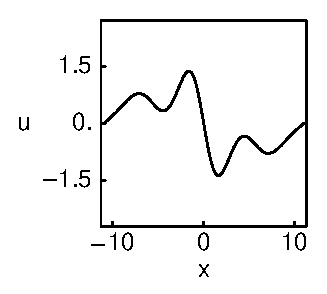
\includegraphics[width=0.35\textwidth, clip=true]{1wKS22equil}
~~~~(\textit{b})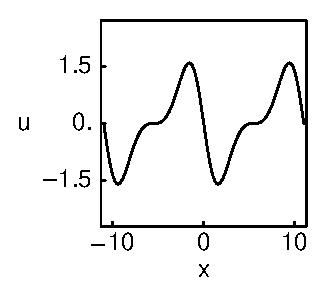
\includegraphics[width=0.35\textwidth, clip=true]{2wKS22equil}
\\
  (\textit{c})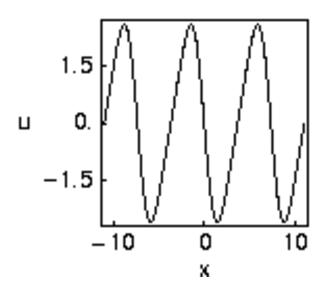
\includegraphics[width=0.35\textwidth, clip=true]{3wKS22equil}
~~~~(\textit{d})\includegraphics[width=0.35\textwidth, clip=true]{equilSpatial}
\end{center}
\caption{
(a) \EQV{1}, (b) \EQV{2}, and (c)
\EQV{3} \eqva. The \EQV{0} \eqv\ is the $u(x)=0$ solution.
(d) $(u,u_x,u_{xx})$ representation
of (red) \EQV{1}, (green) \EQV{2},  (blue) \EQV{3} \eqva,
(purple) \REQV{+}{1},  and (orange) \REQV{-}{1} \reqva.
$L=22$ system size. From Cvitanovi{\'c}, Davidchack and Siminos\rf{SCD07}.
    }
\label{SCD07f:KS22Equil}
\end{figure}
%%%%%%%%%%%%%%%%%%%%%%%%%%%%%%%%%%%%%%%%%%%%%%%%%%%%%%%%%%%%%%%%


Also, I'm unsure whether my code is having a harder time finding \twot\ spatiotemporal
invariant solutions at larger domains or if its just a consequence of punctuating
the runs more often to make more tuning and corrections.



\PCpost{2018-05-30}{Some logical cross-checks:
The  \KSe\ is Galilean
invariant: if $u(x,t)$ is a solution, then $v+u(x-vt,t)$, with $v$ an
arbitrary constant velocity, is also a solution.
In our fixed $L$ calculations we only work in the zero mean velocity
frame, so let us also require that in $L\to\infty$ limit
\beq
\int dx \, u = 0
\,.
\ee{DasBuch:GalInv}
Suppose that
\beq
\oint dx \, u_p = C_p \neq 0
\ee{DasBuch:GalInvNonZero}
for a given \twot\ $p$. But that cannot tile the infinite space
\refeq{DasBuch:GalInv}, as each repeat over
a segment of length $L$ increments the integral by $C_p$. Hence it
is OK to demand that $\expct{u}=0$ vanishes for every solution $p$.

Note also that $\expct{u}=0$ implies that the energy density is proportional
to twice the variance of $u$,
\beq
\sigma^2
   = \expct{(u-\expct{u})^2}
   = \expct{{u}^2}
\,.
\ee{variance}
This quantity is a ``random walk'' in $u$, and expected to grow linearly with
$L$, so the energy density \refeq{SCD07ksEnergy} is expected to go to a limit
for $L\to\infty$, justifying the rescaling of $u$ proposed above. That also
means that the range of $u$ values for a typical \reqv\ should (could?) grow
linearly with $L$, and for a typical \twot\ proportionally to $L\period{}$.

The reason I obsess about this is that we need to have the same (covering)
alphabet everywhere. So our letters should correspond to local \emph{increments} (like
the turns of the unstable spiral around the equilibrium $c_{-}$),
and not be proportional to the magnitude of $u$.
}

\MNGpost{2018-05-31}{
Having trouble finding the magic bullet for rescaling \eqva.
I believe that the correct transformation for rescaling
$u$ in \refeq{SCD07eq:stdks} is $u \to u_p\sqrt{2 \expctE_p}$,
rather than Predrag's \(u \to u_p\sqrt{\expctE_p}\).

This can be seen by looking at the equilibrium condition of \refeq{rescal:eq:stdks}.
If the solution has spatial derivatives equal to zero, then \refeq{rescal:eq:stdks}
implies $\frac{1}{2}u_p^2 = 1$, which in turn implies $u_p^{\pm} = \pm \sqrt{2}$.
    }

\MNGpost{2018-05-31}{
Therefore, I believe the correct transformation is  \(u \to u_p\sqrt{2 \expctE_p}\),
which leads to
\beq
u_p^2 + \sqrt{\frac{2}{\expctE_p}}(- c u_p + u_{p,x} + u_{p,xxx})=1
\,,
\label{rescal:eq:stdks2}
\eeq
rather than Predrag's
\refeq{rescal:eq:stdks}.
    }


With my rescaling, the {\eqv} points of \refeq{SCD07eq:stdks} are now
\beq
c_{+}=(\frac{1}{\sqrt{2}},0,0)\,,\qquad c_{-}=(-\frac{1}{\sqrt{2}},0,0)
\,,
\ee{EqvEqvPtsRscMNG}
After further investigation and numerous checks the rescaling by the now
corrected value still doesn't seem to work
for \eqva\ solutions on arbitrary domain sizes. The issue seems to be
that solutions bifurcate via crossing over $(0,0)$ in the rescaled
$(u_p,u_{p,x})$ axes, almost in the act of shedding loops that
do not follow the symbolic dynamics prescribed by looping around the equilibria
at $(\pm 1,0,0)$.

\MNGpost{2018-05-31}{
Animation \HREF{../figs/eqva_bif.gif} {../figs/eqva\_bif.gif}
(run it in Chrome or in Photoshop or the like)
shows the change of an \eqv\ identified in the next post with increasing the domain
size from $L=12$ to $L=32$ through numerical continuation (as opposed to hundreds
of ``slides"). The left frame is a plot $(u_p,u_{p,x})$, and the right frame
plots $(x,u_p(x))$. The domain size is indicated in the title of each plot.
Note that $u_p$ are the \PCedit{\emph{rescaled}} fields, as defined  by
\refeq{rescal:eq:stdks}.

The domain size was numerically continued by using spatiotemporal (overkill)
convergence code that fixes the domain size, unlike my other codes. The
domain size was changed in step sizes of $\Delta L = 0.1$. It converged over
the range of $L \in [12,32]$, which suffices to identify several bifurcations.
}

\PCpost{2018-06-19}{
{\bf \HREF{../figs/eqva_bif.gif} {../figs/eqva\_bif.gif} narrative}\\
Much is known about what one expects, see \reffig{fig:SCD07ksBifDiag}.
In the natural units  $\tildeL = L/2\pi$ of system size length,
%(not one graduate student in the history of this project would do that),
one finds zero-energy bifurcations off the \eqv\ $u(\conf,\zeit)=0$
at integer $\tildeL=1,2,3,4,5,\cdots$, \ie, at\\
$L=6.283,12.566,18.849,25.133,31.416,\cdots$

As $\expctE$ is here a very important parameter that vanishes at the birth of
\eqva\ spun off $u(\conf,\zeit)=0$, one should \emph{not rescale} $u$ by
\refeq{rescal:eq:stdks} in these plots. A look at Kevrekidis, Nicolaenko and
Scovel\rf{KNSks90} Fig.~6.1 indicates that the same maxima
$\expctE=1.6\cdots$ for \EQV{k}, $k=1,2,3$ are only apparently the same, maxima
do grow larger for for larger $k$.

The initial $L=12$ \eqv\ is \EQV{1}. It collides with a pure harmonic at
$\tildeL=2.013$ (known as $L=12.65$ in gradstud speak). We see from
\reffig{fig:SCD07ksBifDiag} that is the death of \EQV{1} and its continuation
as \EQV{2}. In turn, \eqv\ \EQV{2} dies someplace above $L>25$ (details might
be in the literature). Matt's continuation misses all other coexisting \eqva\
and \reqva, unless it picks up the bifurcation to \eqv\ GLMRT\rf{ksgreene88} at
$\tildeL=2.5\cdots$ (known as $L=15.7\cdots$ in gradstud speak). But I am unsure as
to it actually doing that.
\PC{2018-06-20}{
According to Greene and Kim\rf{ksgreene88}, GLMRT solutions (studied at
length by them) are generalized LMRT solutions of LaQuey \etal\rf{laquey74},
where ``LMRT'' are the author initials, and decoding what they would
correspond to today, 45 years later, we leave as an exercise to the reader.
    }

Next, something happens at $\tildeL=3.63$ (known as
$L=22.8$ in gradstud speak). Perhaps GLMRT $\to$ \REQV{\pm}{1}. That will
be easy to tell if also $\expctE$ is plotted as a function of $L$.
}

\MNGpost{2018-06-05}{
Currently running testing to determine how many spatiotemporal modes are needed for accurate representations of
{\twots}. Running tests where $L=23$ with the number of spatial modes is $m=16$ which
has been shown before to be adequate at this domain size. Although I have code running I have yet to find to most
convincing way of demonstrating where the temporal discretization is adequate, convergence doesn't seem to be the
best means of demonstrating this because solutions can converge with a small temporal discretization but when
viewed qualitatively sometimes even the converged solutions do not look like what I would expect.

This falls under the title of tuning and testing of the spatiotemporal codes; trawls still being run on light to find shift-reflect {\twots}, as I wasn't sure where the error of \rpo\ {\twots} was. Will start \rpo\ {\twot} trawls tomorrow, also need to upload more figures from further trawls, although as the domain size increases the number of convergent solutions seems to be decreasing.

After further testing, imposing the correct spatial scale as determined by the spectrum of the \KSe\
$\tilde{L} = 2\pi \sqrt{2}$ leads to many \eqva\ solutions so imposing the incorrect spatial scale is almost more
beneficial much like imposing a larger than normal magnitude of the spatiotemporal field $u(x,t)$.
}

\MNGpost{2018-06-11}{{\bf Trawling}
on larger domains $L > 70$ is picking up nothing but bottom feeders currently
so I've been working on improving the trivial symmetry, \ie\ full {\statesp} code
in hopes that relaxing symmetry requirements finds us more \twot\ invariant doubly
periodic solutions. Other than the \rpo\ \twot\ solutions posted today there is only
one new \ppo\ \twot\ solution before I left the office so I'll wait for a bigger haul before
uploading.
}

\MNGpost{2018-06-11}{{\bf Numerics: aliasing}
Extracted information from \refref{Canuto88} on what I thought was one of the gaps in my code
which was the fact that it seemed to perform much better as a fully aliased pseudospectral
calculation rather than a de-aliased calculation. I feared that this would bring criticism
so as I tried to armor myself by actually \emph{reading}. My argument is that while aliasing
can be devastating for temporal evolution due to the contamination of the higher Fourier
mode components by their aliases, ($k' = k + N$) where $N$ is the number of collocation
points, the spatiotemporal problem should be fine as long as the calculation is well
resolved enough. In fact, this is likely why I have solutions that "converge" on larger
spatial domains than the discretizations can seem to resolve.

Aliasing commments:
\begin{quote}
For evolution problems  one must address the issue of the temporal numerical
stability of the calculation. Collocation approximations must be formulated
with more care than Galerkin approximations. The reason is that for evolution
problems with quadratic conservation properties, the Galerkin formulation
will automatically yield semi-discrete quadratic conservation laws.
\end{quote}

\begin{quote}
Numerous comparisons have been performed for aliased and de-aliased
calculations of the periodic, multidimensional Navier-stokes equations.
Useful discussions may be found in
\rf{Orszag72,FoxOrs73,Montigny82,Kerr85}.  All of these authors conclude
that with sufficient resolution, aliased calculations are quite acceptable.
\end{quote}


\begin{quote}
Moser, Moin and Leonard\rf{MML83} caution against aliased calculations.
They present a single, poorly resolved, aliased calculation and compare it with three
de-aliased calculations, one poorly resolved, one moderately resolved, and one well
resolved. Their single aliased result is certainly much worse than their well resolved,
de-aliased case, but their poorly resolved, de-aliased case is no better than the aliased
one. Hence, their conclusion is not supported by their evidence.
\end{quote}

In light of these comments and discussions I believe that de-aliasing is more
important in the context of accurate temporal evolution, but not required in
the spatiotemporal fixed point problem as long as the patterns are
sufficiently resolved. One way of thinking about this is that in the
discretization of the spatiotemporal \KSe\ we could add a term that
represents the aliasing,
\[
\sum_{m',n'}\sum_k\neq 0,j\neq 0 a_{m-m'+kM,n-n'+jN}a_{m+kM,n+jN}
\,,
\]
as it is implicit in the fully aliased representation of the equations.

I believe the spectrum of the \KSe\ plays a role, and it might be wise to at
least dealias the temporal convolution sum as there is less of a precedent
for ignoring it; In the spatial case we can at least claim the hyperdiffusion
term diminishes the amount of corruption in the spatial wave number, but this
is harder to motivate for the temporal terms.

More motivation from Canuto, Hussaini, Quateroni and Zhang\rf{Canuto88} are
their fig.~7.1 and fig.~7.4, where the fully aliased but more resolved terms seem
to beat out even the dealiased computations in energy conservation of the KdV
equation for fig.~7.1.

Their fig.~7.4 is a reproduction of the effects of aliasing in the transition
to turbulence in channel flow by  Krist and Zang\rf{KrZa87}. Only the high
resolution (aliased) seems to be physically representative of the actual
solution, and even the dealiased computation on a coarser discretization
(while better than the equivalent aliased discretization) still does not
prevent artificial oscillations. This is also a temporal evolution problem
which we are not dealing with.

In light of all that I have seen, resolution is King.
    }


\begin{figure}
\begin{minipage}[height=.32\textheight]{.5\textwidth}
\centering \small{\texttt{(a)}}
\includegraphics[width=\textwidth,height=.32\textheight]{MNG_eqva_rescaled_proto}
\end{minipage}
\begin{minipage}[height=.32\textheight]{.5\textwidth}
\centering \small{\texttt{(b)}}
\includegraphics[width=\textwidth,height=.32\textheight]{MNG_eqva_rescaled_proto_zoomed}
\end{minipage}
\caption{ \label{fig:MNG_eqva_proto}
(a) Plots of $u_p$ versus $u_{p,x}^2-u_{p,xxx}^2$ for all of the \eqva\ solutions in svn repository.
(b) Zoomed in view showing that all spatial periodic orbits seem to intersect at
$(\pm 1, 0)$ in these coordinates.
}
\end{figure}

\begin{figure}
\begin{minipage}[height=.32\textheight]{.5\textwidth}
\centering
\includegraphics[width=\textwidth,height=.32\textheight]{MNG_eqva_family_return}
\end{minipage}
\begin{minipage}[height=.32\textheight]{.5\textwidth}
\centering \small{\texttt{(b)}}
\includegraphics[width=\textwidth,height=.32\textheight]{MNG_eqva_family_return_zoomed}
\end{minipage}
\caption{ \label{fig:MNG_eqva_family_returnmap}
(a) Return map of  $u_{p,x}^2-u_{p,xxx}^2$ for a family of \eqva\ numerically continued in space. Found by looking for when the other transformed coordinate $2u_{p,x}u_{p,xxx}$ passes through zero and $u_{p,x}^2-u_{p,xxx}^2$ is positive. (b) Window around the origin. Color scale indicates the domain size of the numerically continued \eqva\
}
\end{figure}

\begin{figure}
\begin{minipage}[height=.32\textheight]{.5\textwidth}
\centering
\includegraphics[width=\textwidth,height=.32\textheight]{MNG_eqva_return}
\end{minipage}
\begin{minipage}[height=.32\textheight]{.5\textwidth}
\centering \small{\texttt{(b)}}
\includegraphics[width=\textwidth,height=.32\textheight]{MNG_eqva_return_zoomed}
\end{minipage}
\caption{ \label{fig:MNG_eqva_returnmap}
(a) Return map of  $u_{p,x}^2-u_{p,xxx}^2$ for all \eqva\ in svn repository. Found by looking for when the other transformed coordinate $2u_{p,x}u_{p,xxx}$ passes through zero and $u_{p,x}^2-u_{p,xxx}^2$ is positive. (b) Window around the origin. Color scale indicates the domain size of the \eqva\ .
}
\end{figure}

\MNGpost{2018-06-11}{{\bf \Eqva\ rescaling}
I've been trying to work with the rescaled equation for \eqva\ of the $T=0$
system in order to best demonstrate how they are organized in space. Burak
pointed out that I should be able to get a lobe if I use the Miranda and
Stone\rf{GL-Mir93} coordinate transformation (discussed at length in
ChaosBook for the Lorenz symmetry reduction). I'm still playing around with
it but here are the best results I have so far:
\begin{itemize}
\item
\refFig{fig:MNG_eqva_proto} is a plot of $u_{p,x}^2-u_{p,xxx}^2$ as a
function of $u_p$. Other projections don't seem to elucidate anything and
when zooming in even further than (b), all orbits come within about $10^-7$
of intersecting $(\pm 1, 0)$ in terms of vertical ($u_{p,x}^2-u_{p,xxx}^2$)
distance.
\item
\refFig{fig:MNG_eqva_family_returnmap} finds the return map of
$u_{p,x}^2-u_{p,xxx}^2$ of a family of numerically continued \eqva\ solutions
in space by calculating when the other nonlinear coordinate transformation $v
= 2u_{p,x}u_{p,xxx}$ crosses the origin, with $u_{p,x}^2-u_{p,xxx}^2$
positive, to guarantee that all section crossings are in the same direction.
Color coding indicates domain size of the solution.
\item
\refFig{fig:MNG_eqva_returnmap} The return map calculated as in
\reffig{fig:MNG_eqva_family_returnmap} but with all of the \eqva\ solutions
in the repo.
\end{itemize}

Whether these plots will prove useful for analysis is still to be seen.
\refFig{fig:MNG_eqva_proto} might help. While its not as
clear as to how to formulate the symbolic dynamics as in the Lorenz system,
as there seem to be three distinct lobes as opposed to two; in the symmetry
reduced projection it might change from a three-letter alphabet to a two
letter alphabet; What I'm trying to say is that by using this coordinate
transformation, even when plotted in a non-reflection symmetry reducing way I
believe that there are three lobes, \ie, $(-1,C,1)$, which might be useful.
}

\MNGpost{2018-06-11}{{\bf Reading}
While making small coding adjustments and playing with \eqva\ of \eqva\ I've
been trying to read as much on the variational integrator literature as I
can; there's just a lot. Kraus and Maj\rf{KraMaj15} seems to be a good
introduction but there the notation is seemingly purposefully confusing. Due
to the geometrical nature there are lots of indices and substitutions and man
I find it hard to get through the brush.
}

\begin{figure}
\begin{minipage}[height=.32\textheight]{.5\textwidth}
\centering \small{\texttt{(a)}}
\includegraphics[width=\textwidth,height=.32\textheight]{MNG_ppo_subdomains}
\end{minipage}
\begin{minipage}[height=.32\textheight]{.5\textwidth}
\centering \small{\texttt{(b)}}\\
  \begin{minipage}[height=.16\textheight]{.44\textwidth}
    \centering \small{\texttt{Defect1}}
    \includegraphics[width=1.2\textwidth,height=.16\textheight]{MNG_rpo_L13d2_T15}
  \end{minipage}
  \begin{minipage}[height=.16\textheight]{.44\textwidth}
    \centering \small{\texttt{Defect2}}
    \includegraphics[width=1.2\textwidth,height=.16\textheight]{MNG_rpo_L17d5_T17}
  \end{minipage}
  \begin{minipage}[height=.16\textheight]{.44\textwidth}
    \centering \small{\texttt{Streak}}
    \includegraphics[width=\textwidth,height=.16\textheight]{MNG_eqva_L8d5}
   \end{minipage}
  \begin{minipage}[height=.16\textheight]{.44\textwidth}
    \centering \small{\texttt{Gap}}
    \includegraphics[width=1.2\textwidth,height=.16\textheight]{MNG_gap}
  \end{minipage}
\end{minipage}
\caption{ \label{fig:MNG_ppo_subdomains}
(a) A proposal for an alphabet of \KS\ spatiotemporal patterns with
catchy names. One should also quotient the spatial reflection, \ie,
the fundamental domain is 1/2 of the pattern shown.
(b) Corresponding representative \twots:
defect1 = \RPOtwot{13.2}{15}; %\emph{rpo\_L13.2\_T15};
defect2 = \RPOtwot{17.5}{T17}; %\emph{\emph{rpo\_L17.5\_T17};
streak = \emph{eqva\_L8.5};
gap = \PCedit{\emph{po\_L17.3\_T15.3}}.
}
\end{figure}

\begin{figure}
\begin{minipage}[height=.32\textheight]{.5\textwidth}
\centering \small{\texttt{(a)}}
\includegraphics[width=\textwidth,height=.32\textheight]{MNG_ppo_frankenstein}
\end{minipage}
\begin{minipage}[height=.32\textheight]{.5\textwidth}
\centering \small{\texttt{(b)}}
\includegraphics[width=\textwidth,height=.32\textheight]{MNG_ppo_L30_T44}
\end{minipage}
\caption{ \label{fig:MNG_frankenstein}
(a) A crude tiling of a
(b) shift-reflect invariant \twot\
\PPOtwot{30}{44} %\emph{ppo\_L30\_T44}
.
This uses only snippets from \reffig{fig:MNG_ppo_subdomains}.
Continued in the blog post of {\bf 2018-11-09}.
}
\end{figure}


\MNGpost{2018-06-25}{
Working through using CUDA (Nvidia based GPU processing toolkit) for
energy norm comparison code.

The outline of the code is as follows,
\begin{itemize}
\item Produce large scale (``infinite") spatiotemporal computations with
a spatiotemporal discretization convention such that $\Delta x, \Delta t = 1$, for instance.
\item Rediscretize {\twots} to obey the same discretization convention.
\item Either use spatiotemporal \twot\ solutions or subdomains to search for regions where
difference in energy norm is small.
\item Do the energy norm computations in parallel so that it runs fast.
\item Produce figure by cutting out where the difference in energy norm is small comparatively,
label with symbol.
\end{itemize}

From staring at {\twots} there are a few tiles that seem to appear
frequently, see \reffig{fig:MNG_ppo_subdomains}.
Any of these patterns could also have an additional adjective ``tilted" in front
of them, which is the same shape with the addition of \SOn{2} rotation:
\begin{itemize}
\item Streaks (\eqva, \reqva)
\item Defects ($2\rightarrow 1$ wavelength mergers)
\item Hooks
\item Half defect/half hook (birth and death timescales for each ``half"
                             of the merger are drastically different)
\item Bent streaks
\item Gaps
\end{itemize}

I believe that there is a physical way of explaining the pattern
formation of the defects in \ppo\ {\twots}. It
begins when the spatial domain size becomes large enough that it can
admit an additional pair of streaks (crest and trough), due to a higher
spatial wavenumber becoming the most unstable. What I believe happens
next is that the streaks bend giving rise to a spatiotemporal region that
is for all intensive purposes ``empty" of structure ($u=0$). Because the
\KSe\ is linearly unstable, the region becomes a site for the formation
of a new defect. It begins first with the formation of a ``hook" branching
off from its original streak. As the magnitude of the crest and trough
combination grows, it detaches from its original streak, leading the the
``half-hook" or ``half-defect" structure. I am categorizing this by ``half"
because the time-scales for birth and death of the defect are drastically
different. Eventually the half defect merges with another streak, leading
to the full $2\rightarrow 1$ wavelength merger, where both halves of the
defect have the same time scale. I don't know how to include rotations
into this impromptu theory, but in my mind they just allow more
combinations of possible streak and half-defect mergers.
}

\PCpost{2018-06-27}{
The love child \reffig{fig:MNG_frankenstein} of many genders of spacetime
patches is cute! Let's try to find \twots\ that capture these shapes.
(Continued in the blog post of {\bf 2018-11-09}.)
}

\PCpost{2018-06-27}{
Looking at \\
\texttt{gudorf/python/KSTori/converged\_solutions/figures/}:
% \texttt{ppo/}, \texttt{rpo/}.
\begin{enumerate}
  \item[\texttt{eqva/}]
Need to know energy densities - perhaps a single \texttt{E.txt} list would suffice.

$u(x)=0$ solution: eqva\_L26.9

  \item[\texttt{eqva/figsWide}]
$u(x)=0$ solutions: eqva\_L494.5,  eqva\_L594.7,
          eqva\_L597.3,  eqva\_L625.7,  eqva\_L628.2,  eqva\_L666.1,  eqva\_L676.8,
          eqva\_L703.8, eqva\_L751.4, eqva\_L813.2
  \item[\texttt{reqva/}]
Need to know energy densities and travelling wave velocities - perhaps \texttt{E.txt},
\texttt{c.txt} lists would suffice.

$u(x)=0$ solutions: reqva\_L24.9, reqva\_L32.1, reqva\_L44.3,
  \item[\texttt{full/}]
What is ``\texttt{full/}?'' A periodic orbit? If in $\bbU^+$, I would
expect those should be antisymmetric under a space reflection, but I do
not see the symmetry line for any of them, except for
\PPOtwot{34.9}{23}, %ppo\_L34.9\_T23,
full\_L26.7\_T54,
full\_L32.5\_T19

%$u(x)=0$ solution (?): full\_L43.3\_T41

%  \item[\texttt{rpo/}]
%Need to know energy densities and mean phase velocities - perhaps \texttt{E.txt}
%\texttt{c.txt} lists would suffice.
%
\end{enumerate}
I moved all $u(x)=0$ solutions to \texttt{zero/}.
}

\PCpost{2018-06-29}{
moved from \emph{eqva/dataWide} to \emph{eqva/data}:\\
    eqva\_L56.4, eqva\_L56.9, eqva\_L77.7

% currently missing from \emph{eqva/figs}:    eqva\_L26.9
% currently missing from \emph{reqva/figs}:
    % reqva\_L24.9, reqva\_L32.1, reqva\_L44.3
% \MNGedit{These were moved to \emph{zero/figs} on 2018-06-26}.
% PC moved the data files to zero/data/
}

\MNGpost{2018-06-28}{``Full" was what I called the periodic orbits that
were found with \refeq{eqn:MNGspacetime_mvf} that had a $\SOn{2}$ shift
that was smaller than the grid spacing, \ie, $\sigma \leq \frac{L}{M}$, I
realized after looking at the trawls that my \rpo\ \twot\ codes did not
have any guarantee they were picking out prime periods and some of the
solutions look spurious.
}

\PCpost{2018-06-27}{
\texttt{eqva/} $k$ wavenumber ``streak'' tiles:


eqva\_L22.4 is 2 repeats of eqva\_L11.2, find it.

eqva\_L23.8 is 2 repeats of eqva\_L11.9, find it.

eqva\_L25.5 is 4 repeats of eqva\_L6.37, find it.

eqva\_L25.7 is 3 repeats of eqva\_L8.6, find it.

eqva\_L29.4 is 4 repeats of eqva\_L7.35, find it.

eqva\_L34.1 is 3 repeats of eqva\_L11.4, find it.
}

\MNGpost{2018-06-28}{
All were found. As they belong to continuous families,
I found them at slightly different lengths.
}

\PCpost{2018-06-27}{
\texttt{full/} $(L/3,T/3$ shift and translate ``cat eye'' or ``gap'' tiles:

full\_L24.4\_T41 seems ``almost'' invariant under
$x \to x -L/3,$ $t \to t + 2\period{}/3$ and
$x \to x  L/3,$ $t \to t +  \period{}/3$.

Matt, can you find a solution
\PPOtwot{8.1}{13.7} %ppo\_L8.1\_T13.7
with 1/3 shifts both in space and time?

Similarly,
\PPOtwot{25.3}{13.7} %ppo\_L25.3\_T13.7
seems ``almost'' invariant under
$x \to x -L/3,$ $t \to t +  \period{}/3$ and
$x \to x  L/3,$ $t \to t + 2\period{}/3$.

Matt, can you find a solution
\PPOtwot{8.4}{7.3} %ppo\_L8.4\_T7.3
with 1/3 shifts both in space and time?

In other words, both are the same solution, differing only in $E$.
This ``cat eye'' appears many places, for example in
\PPOtwot{24.4}{17}, %ppo\_L24.4\_T17,
\PPOtwot{24.4}{41}, %ppo\_L24.4\_T41,
\RPOtwot{26.8}{21}, %rpo\_L26.8\_T21,
\RPOtwot{24.5}{55}, %rpo\_L24.5\_T55,
\RPOtwot{24.9}{74}, %rpo\_L24.9\_T74,
\PPOtwot{30.6}{12}, %ppo\_L30.6\_T12,
\RPOtwot{31.1}{85}, %rpo\_L31.1\_T85,
\PPOtwot{31.8}{40}. %ppo\_L31.8\_T40.
    }

\PCpost{2018-06-27}{
$k \to k-1$  ``defect'' tiles: They look
like temporally heteroclinic connections, not sure it makes sense to make the
spatiotemporaly periodic. Still,
\RPOtwot{28.6}{12} %rpo\_L28.6\_T12
suggests Matt might find be a
\RPOtwot{14.3}{12}, %rpo\_L14.3\_T12
single ``defect tile.''
}

\PCpost{2018-06-27}{
When they go high, we go low. Try to find a set of \twots\ with the smallest possible
$L$ and $T$.

Keep track of energy density $E$ - some of the above are related by
continuation. We have to figure out what selects a preferred solution
from a continuous family with differing $E$.

In all of the above searches - never start by a random initial condition, always use
patches of the existing solutions (perhaps smoothed out by a Fourier transform,
throw away high wave numbers, Fourier transform back) as the initial conditions.
}


\MNGpost{2018-06-29}{
%Still working on the work required to fulfill the requests made in previous posts.
The fact the defects come in continuous families isn't too surprising but
it makes analysis a little harder. The idea that I've been thinking
through is to use {\twots} to create a library of these
patterns, but they emerge in all of the spatiotemporal patterns.
}

\PCpost{2018-06-29}{
Try to find the above {\bf 2018-06-27 Predrag} shortest time \\
rpo\_L14.3\_T12
$k \to k-1$  ``defect'' tile (extracted from rpo\_L28.6\_T12?). Then
other defects might be interpreted as streaks (of varying duration) capped
by the defect that might then be again followed by a streak.
}

\MNGpost{2018-06-29}{
I don't have a very robust justification for it just yet, but I believe
the constituent blocks need to be cropped from minimal time and space
solutions, I'm thinking this way because the smaller the spatiotemporal
domain the less likely that rotations come into effect and the I believe
we are more likely to get prime tilings this way. The evidence for this
is by looking through my solutions it seems that if given the leeway in a
larger temporal domain they tend to drift; even though we are in the
shift-reflect invariant subspace I believe the key way of thinking about
this is that the mean shift is equal to zero but not the instantaneous
shifts. Therefore, in small temporal strips the periodic boundary
conditions provide a purer realization of the subdomains.
}

\MNGpost{2018-06-29}{
I'm including animation
{\bf \HREF{../figs/MNG_ppo1_energy.png}
          {../figs/MNG\_ppo1\_energy.png}},
a continuation of {\bf 2018-06-19 Predrag}
\HREF{../figs/eqva_bif.gif} {../figs/eqva\_bif.gif} narrative.
Again, it
runs in Chrome and can be edited in Photoshop.

The idea is that by numerically continuing \PPOtwot{22}{10.2} of the $L=22$
domain, we track the energy of the {\twot} via the
diagonalized quadratic norm of the spatiotemporal Fourier coefficients
and plot them together.

In the animation, the only weak spot is that the extent of time is fixed;
it seems like the best solution to having multiple subplots, one of which
I wanted to demonstrate ``growing". I.e. the $u$ field's spatial extent is
displayed as growing as it should be; sacrificing the aspect ratio
between time and length in the process, so be wary of time scales.

From the plotting, and surprising amount of numerical continuations I was
able to achieve if I stepped over $L=18.6$ (For whatever reason it
couldn't converge at that exact fixed length). I believe the animation
shows that at bifurcations the energy as a function of domain size
remains continuous but not differentiable, as indicated by the kinks at
$\tildeL={L}/{2 \pi} \approx 2.7, 2.9,3.7$.

The idea of this was to show that numerical continuations of a single
\twot\ solution display the different types of defects based on domain
size, but it seems bifurcations are at play here. The cat's eye (gap)
that appears from bifurcating from the equilibrium solutions at small $L$
occurs first, followed by a descent in energy that by eye seems to
approach the antisymmetric subspace $\bbU^+$ (before and after
$\tilde{L}\approx 2.9$. might be two different solution curves but I'm
not convinced). Then as we approach the \ppo\ we are familiar with, the
hook shape seems to form and as we get to large it transitions to the
"half defect" state followed by another bifurcation I believe that leads
to the full defect.

I'm trying to use this as evidence that certain shapes fundamentally
exist in certain spatiotemporal areas, but it's hard to specify due to
the families they come in.
}

\PCpost{2018-06-29}{
An attempt at
{\bf \HREF{../figs/MNG_ppo1_energy.png}
          {../figs/MNG\_ppo1\_energy.png} narrative}:

The antisymmetric subspace \EQV{1} family $\in\bbU^+$ (or
$-u_{\EQV{1}}$, note the tilts are a reflection of each other) in
\HREF{../figs/eqva_bif.gif} {../figs/eqva\_bif.gif} is
followed up to $\tildeL\approx 2.7$, followed by a
spatiotemporal bifurcation to

antisymmetric subspace $\bbU^+$ ``cat eye'' or ``gap'' at $\tildeL\approx
2.9$, followed by spatial-reflection symmetry breaking bifurcation to

``hook'' at $\tildeL\approx 2.9$ (known as \PPOtwot{22}{10.2} at $L=22$),
followed by bifurcation to

``defect'' at $\tildeL\approx 3.7$.
}

\MNGpost{2018-06-29}{:
Found the \eqva\ solutions from {\bf 2018-06-27 Predrag}. Slight
discrepancies in predicted length due to allowing it to vary as a
parameter. I took the original \eqva\ solutions that seemed to be made of
repeats and then took the fraction of the spatial domain given by
1/(number of repeats). For some of the \eqva\ solutions no work
was needed, in this case, the residual of the cost functional after
chopping up the repeated solution was already within machine precision.

For \eqva\, the equations that define the cost functional for the  $T=0$
\KSe\ in terms of (purely imaginary) spatial Fourier modes are
\beq \label{eqn:Fks_eqva}
F_{eq} = (q_m^2 - q_m^4)b_m + \frac{q_m}{2}\sum_{k=0}^{M-1} b_m b_{k-m} = 0
\eeq
with the the cost functional
\beq \label{eqn:eqva_costfunc}
S = \frac{1}{2}F_{eq}^{\top}F_{eq}
\,.
\eeq
I was able to find all prime (spatial) period \eqva\ that Predrag
predicted, but the domain sizes vary slightly as the solutions come in
continuous families.
}

\PCpost{2018-06-29}{
\texttt{wegolow/eqva/figs/}
are all the standard issue, antisymmetric space $\bbU^+$ solutions, so their
actual, prime spatial period is $L/2$ (all that needs to be plotted),
where $L$ is the length Matt currently assigns them.

eqva\_L6.3, eqva\_L7.1, eqva\_L8.5, and eqva\_L11.2 are presumably the
same solution, different $E$'s.

I think this should be the \EQV{1} family (or
$-u_{\EQV{1}}$) in
\HREF{../figs/eqva_bif.gif} {../figs/eqva\_bif.gif}.

eqva\_L11.1 and eqva\_L11.9 are presumably the same solution,
different $E$'s.

If $u_{\EQV{}}$ is a solution, is $-u_{\EQV{}}$ a solution?
I vaguely remember that in the restriction to the antisymmetric
subspace $\bbU^+$, these appear as shifts by $L/2$?

Defect1 \emph{rpo\_L13.2\_T15} looks like a \po\ in the antisymmetric
subspace $\bbU^+$, not like a \rpo. The effect after a $\period{}$ is a
shift by $L/4$: note, no change in the wavenumber.
}

\begin{figure}
\begin{minipage}[height=.32\textheight]{.5\textwidth}
\centering \small{\texttt{(a)}}
\includegraphics[width=\textwidth,height=.32\textheight]{MNG_gapfull}
\end{minipage}
\begin{minipage}[height=.32\textheight]{.5\textwidth}
\centering \small{\texttt{(b)}}
\includegraphics[width=\textwidth,height=.32\textheight]{MNG_gapsub1}
\end{minipage}
\begin{minipage}[height=.32\textheight]{.5\textwidth}
\centering \small{\texttt{(c)}}
\includegraphics[width=\textwidth,height=.32\textheight]{MNG_gap}
\end{minipage}
\caption{ \label{fig:MNG_catseyefigs}
(a) \twoT\ full\_L26.7\_T54.
(b) A temporal subtile that was cut out from (a) and then converged via
    Gauss-Newton method.
(c) The final ``gap" tile, \reffig{fig:MNG_ppo_subdomains},
    that was cut out from (b) and then converged
    to \twot\ \PCedit{po\_L17.3\_T15.3} via Gauss-Newton method.
}
\end{figure}

\MNGpost{2018-07-04}{

\begin{description}
\item[Plumbing? I'm here to tile the walls]
Detailing the process by which I found the tile which is currently being
referred to as ``gap" or ``cat's eye".

I followed the following procedure;
\begin{itemize}
\item
    Look through figures of converged \twot\ solutions for what could
    hold a minimal spatiotemporal tile.
\item
    Note that full\_L26.7\_T54 in \reffig{fig:MNG_catseyefigs}\,(a) seems
    to have a subdomain $\frac{x}{2\pi} \in [0,2.75]$, $t \in [0,18]$
    that is the ``gap" or ``cat's eye" pattern.
\item
    To be safe, first truncate the temporal extent only, and converge the
    solution. This leads to \reffig{fig:MNG_catseyefigs}\,(b), where the
    period takes the new value $T \approx 18.9$, about a third of the
    initial \twot.
\item
    Finally, truncate the spatial extent of
    \reffig{fig:MNG_catseyefigs}\,(b) and converge, resulting in
    \twot\ \PCedit{wegolow/po/po\_L17.3\_T15.3} of \reffig{fig:MNG_catseyefigs}\,(c).
    \PC{2018-07-06}{
    \PCedit{po\_L17.3\_T15.3 is eye-balling guess, please fix,
    provide data file in {\em po/data/}}
    }
\item
    We believe this \twot\ to be a representative ``cat's eye" pattern
    or ``gap'' sketched in \reffig{fig:MNG_ppo_subdomains}, and
    seen frequently in larger \twots.
\end{itemize}

\twoT\ full\_L26.7\_T54, as well as the so far unnamed \twots\
\reffig{fig:MNG_catseyefigs}\,(b) and (c) belong to the antisymmetric
subspace $\bbU^+$, with reflection point $\frac{x^*}{2\pi} \approx 1.25$. The
spatial $\SOn{2}_x$ shift of these solutions is $\shift_x\approx 10^{-5}$.
Because the initial condition for full\_L26.7\_T54 was modulated noise,
and no discrete symmetries was imposed during the calculation, one could
not predict the final symmetry subgroup of a solution when using the
\rpo\ \twot\ spatiotemporal code.

The ``full" type solutions are a subset of solutions to
\refeq{eqn:MNGspacetime_mvf} where the \SOn{2} parameter takes the value
close to zero.
% ; it's hard (meaning I don't know any way) to disallow special subsets
% of possible {\twots} where this is the case.
Using a mean-velocity frame I impose in the ansatz that the \SOn{2}
shift manifests in the equation itself, but there is nothing to prevent
this shift parameter from taking a value of zero, and there is no reason
to fear that either; \reqva\ some in continuous families, with corresponding intervals
of spatial shifts, which can include \po\ $\shift_x=0$ solutions.
%I think to artificially drive it away from zero would be a disaster as I
%have seen frequently that \rpo\ \twot\ solutions will numerically "change
%direction" meaning sometimes an initial net shift in the negative spatial
%direction can switch to a net shift in the positive spatial direction;
%starting from basically nothing means that I can't really impose too many
%constraints or it won't work.

This is similar in regards to the \ppo\ \twot\ spatiotemporal code.
Technically, it can allow for twice repeating solutions in the
antisymmetric subspace $\bbU^+$, but it is quite rare that these events
happen as it requires half of the computational variables,
(spatiotemporal Fourier modes) to be identically zero. An example of this
is
\PPOtwot{34.9}{23}. %ppo\_L34.9\_T23.
    \PCedit{
It is tagged as a \ppo, only the fundamental domain
is being plotted, but it turns out to be a \po\ with
period $T\approx23$.
% If I were to plot the ``full orbit" of ppo\_L34.9\_T23,
% it would easily be seen as a twice repeating antisymmetric solution.
    }

This process is quite idiosyncratic by its nature, and not very easy to
automate as it requires user input to tell what subdomains are good
candidates for minimal tiles. Therefore I hope to have more tiles soon
but its a trudge through messy waters.

\item[Plumbers meeting]
Burak and Elena were present and I think now Burak is on board and
excited about the direction my research is taking; not to say he was ever
opposed to me, let's just be clear. He thinks that it would be beneficial
to develop code that tracks the ``trajectories" of local minima and maxima
through time and plots them might help in terms of analysis. I agree that
while looking at colored density plots of spatiotemporal fields is more
confusing, I'm not sure how easy it would be to implement this type of
code. I believe his idea is that the idea of looking for important
structures, streaks, gaps, etc. comes down to local minima and maxima
pairs, their births and deaths, and one should remove all other
extraneous information. I believe he is in agreement with me that perhaps
numerical continuation of minimal tiles could span a wide enough library
of spatiotemporal symbols such that any solution can be constructed;
where the particular realizations picked from continuous families of
solutions would be determined by \textit{a priori} choosing a
spatiotemporal area to work with.

\end{description}
}

\NBBpost{2018-07-05}{
I really like the patterns in \reffig{fig:MNG_ppo_subdomains}! The solid state
model I mentioned in the earlier meetings is called ``terrace ledge kink
model'' and the
\href{https://en.wikipedia.org/wiki/Terrace_ledge_kink_model}{Wikipedia article}
seems to have a good introduction to the basic ideas. The analogy I had in
mind was roughly the following:
\begin{itemize}
    \item Space-time plot $\rightarrow$ 2D crystal surface
    \item Patterns (defect, streak, etc.) $\rightarrow$
          Crystal defects (kinks, adatoms etc.)
\end{itemize}
One thing that is different is the discreteness of crystal surface as opposed
to the continuous tiling in the $(1+1)-D$ spatiotemporal dynamics, where the
patterns appear in different sizes. Matt nicely illustrated these things in
yesterday's meetings by pointing at frequently appearing patterns and matching
them to the ones that appear along the continuation of the fundamental PPO.

I suggest the following for a systematic classification of the patterns:
Take spatiotemporal plots of the Kuramoto-Sivashinsky dynamics and at each
time slice $\zeit$, detect local minima and maxima. Than connect these local
minima and maxima along the spatiotemporal figure with, say, dashed and solid
lines respectively. Roughly speaking, this is going to be drawing lines along
the middle of red and blue regions of the spatiotemporal visualizations.
Perhaps, some thresholding, such as assuming an $(- \epsilon , \epsilon)$
interval to be $0$ since sometimes there are very pale red/blue peaks.
I mentioned up to this point in yesterday's hangout.
}

\PCpost{2018-07-06}{
I have split \po s
\texttt{full/} folder into\\ \texttt{full/} and \texttt{po/}.

\texttt{full/} belong to the continuous \rpo\ families. They are a subset
of solutions to \refeq{eqn:MNGspacetime_mvf} for which the spatial shift
happens to be close to $\shift_x=0$.

\texttt{po/} solutions,
antisymmetric under a space reflection across symmetry
points $x^*$ and $x^*+L_{Matt}/2$, belong to the
{\em spatially antisymmetric subspace} $\bbU^+$, see
\refsect{sect:antisym_subgroup}. Currently Matt has found only

\PPOtwot{34.9}{23}, %ppo\_L34.9\_T23,
full\_L26.7\_T54,
full\_L32.5\_T19,

but
Christiansen, Cvitanovi{\'c} and Putkaradze\rf{Christiansen97}
($\tildeL \approx 5.8$),
and Lan and Cvitanovi{\'c}\rf{lanCvit07} ($L = 38.5, \tildeL = 6.12$)
have hundreds of them for a few fixed system sizes $L$.
\\
\MNGedit{I have never explicitly searched for antisymmetric solutions
$\in \bbU^+$
because I focused on \ppo\ and \rpo\ solutions. I'll get on the
trawling.}
}

\PCpost{2018-07-06}{ \emph{eqva/figs}:
%The solutions eqva\_L31.3, eqva\_L35.9
%do not look to me (I might be wrong) like they are in the spatially
%antisymmetric subspace. Presumably they are \rpo s whose spatial shift
%happens to be $\shift_x=0$.
%\MNGedit{These were accidentally tagged as \eqva\ and not \reqva\ because
%their \SOn{2} shifts were so small}

The antisymmetric space $\bbU^+$ solutions prime spatial period is
$L_{Matt}/2$. Center them at $x^*=0$ or $x^*+L_{Matt}/2=0$, and the prime
spatial period $[0,L]$ where $L=L_{Matt}/2$ is all that needs to be
plotted, where $L_{Matt}$ is the length Matt currently assigns them.\\
\MNGedit{This has been fixed for \eqva.}
\PC{2018-07-07}{Today they all look centred, but plotted on fundamental
domain and its copy, total width $L_{Matt}$.}
}

%Takes a noticeable time to input large figures; commenting out as surface physics ideas are not
%a priority.
s
%\begin{figure}
%\begin{minipage}[height=.32\textheight]{.5\textwidth}
%\centering \small{\texttt{(a)}}
%\includegraphics[width=\textwidth,height=.32\textheight]{MNG_uu500b500}
%\end{minipage}
%\begin{minipage}[height=.32\textheight]{.5\textwidth}
%\centering \small{\texttt{(b)}}
%\includegraphics[width=\textwidth,height=.32\textheight]{MNG_minmax500b500}
%\end{minipage}
%\caption{ \label{fig:MNG_minmaxtracking}
%(a) Numerically integration of \KSe\ on large spatial domain.
%(b) The result of tracking the minima and maxima of (a).
%}
%\end{figure}

\MNGpost{2018-07-06}{
First attempts at local minima and maxima tracking algorithm. Simon Berman gave me the idea,
which is to take the spatial derivative of the spatiotemporal field represented as a matrix $u_x(x_m,t_n)\equiv a_{m,n}$
and to calculate an elementwise product and subtraction $P_{m,n} = a_{m+1,n}a_{m,n}$ and
$S_{m,n} = a_{m,n}-a_{m+1,n}$ to capture where the derivative changes sign, as well as the sign
of the second derivative approximated by the secant line between spatially adjacent points.

Responses to Predrag's posts:
\begin{itemize}
%\item I found the missing figs, they were in \emph{/zero/figs/}
%\item The \eqva\ that didn't look like \eqva\ were in fact mislabelled
%\reqva\ which slipped through the net because their \SOn{2} shifts (or
%group velocity, however one wishes to label it) were really small.
\item I haven't trawled specifically for antisymmetric \twot\ solutions
$\in\bbU^+$ but can do so, I was focused on \ppo\ and \rpo\ solutions.
\item \eqva\ figures should now reflect the prime spatial period and so
will antisymmetric \twot\ solutions $\in\bbU^+$.
\end{itemize}

}

\MNGpost{2018-07-04}{
{\bf Notes from Monday's Art Institute visit}
Called Predrag via hangouts, we discussed the two hurdles looming ahead
of us in terms of the theory. He says:

\begin{itemize}
\item[0]
WeGoLow, WeGoLow, WeGoLow. We keep determining the alphabet of minimal
tiles, until we have a credibly complete alphabet.
We do not let ourselves get disturbed by Grand Schemes of
Budanurs, get batted out \emph{again} into the far field. WeGoLow,
WeGoLow, WeGoLow, as has been the goal for the last 2 years.

Once we have an alphabet, the conceptual challenges ahead are
\item[1]
Solutions come in continuous families.
Depending on the initial guess, current Matt's code
picks out an arbitrary representatives from such continuous family.
Is there a saddle-point condition (let's say, extremum in energy density)
that picks out a single representative \twot\ per family? Or will
\po\ zeta functions involve integrals over such families?

\item[2]
To a single \twot\ belongs a continuous family of tiles, one for each value
of $(x,\zeit)$ that we take to be the origin of the tile. In other word,
how will we maximize the amount of shadowing of a large \twot\ by smaller
\twots\
\end{itemize}
}

\PCpost{2018-07-07}{
There are tons of intriguing solutions in Matt's library, almost all for
relatively large domains. I think new searches should focus on smaller
and smaller domains, to help the intuition about the alphabet, and fusion
rules - which pattern can be adjacent to which.

Some WeGoLow candidates:

\emph{rpo\_L21.9\_T95} \\
(also
\emph{rpo\_L22.1\_T92},
\emph{rpo\_L22.1\_T93},
\emph{rpo\_L22.2\_T84},
\emph{rpo\_L22.3\_T90},
\PPOtwot{22.3}{96}, %\emph{ppo\_L22.3\_T96},
\emph{rpo\_L22.5\_T89},
\emph{rpo\_L22.5\_T89}):
start a \po\ search using $T=[9,30]$ time clip, or (better)
\ppo\ search using $T=[9,20]$ time clip. From that, start a
\ppo\ search using $L/2\pi=[0.2,2.6]$ space clip. The result could be
WeGoLow
\PPOtwot{15}{11} %ppo\_L15\_T11
``hook'' in \reffig{fig:MNG_ppo_subdomains}.
However, this solution might be rare for larger spatial periods.

\emph{rpo\_L21.9\_T79}\\
(also
\PPOtwot{24.9}{58}, %\emph{ppo\_L24.9\_T58},
\emph{rpo\_L34.8\_T36},
\emph{rpo\_L36.9\_T63},
\emph{rpo\_L42.6\_T62}):
$T=[45,79]$ time clip suggests an interesting
\rpo\ which is the $T=[45,61]$ ``hook" repeated.

\emph{rpo\_L22.1\_T81}: $T=[70,87]$ time clip is an example of $k=3 \to k=1$
defect.
}

\MNGpost{2018-07-10}{
After rewriting/updating the antisymmetric invariant subspace $\bbU^+$
spatiotemporal code, I was able to converge former ``gap'' or ``cat's
eye" tile \emph{ rpo\_L13.2\_T15 } to a \po\ named Defect 2
\emph{anti\_L17.5\_T17} in the antisymmetric invariant subspace, plotted
in $[0,L/2]$ domain.

With restructuring my code into a more presentable package I've found
that there are slight inconsistencies in how python interprets the
"project" whether in Windows or Linux OS. It's this and bug hunting that
are keeping me preoccupied sadly. Also, I went through and wrote most of
the antisymmetric invariant subspace $\bbU^+$ trawling code; analogous to
what I used for \ppo\ and \rpo\ solutions. There seems to be a bug in the
matrix free methods that I haven't found. I know that it lies in this
specific part because the explicit matrix methods worked by producing
defect2 \emph{anti\_L17.5\_T17}. The matrix free code is drastically
altering the domain size and needs more work before I can start trawling.
}

\MNGpost{2018-07-11}{
\begin{description}
\item[coding]
Wrote auxiliary functions to be able to more easily manipulate datasets for
the sake of finding WeGoLow tiles.

\item[Plumbers Meeting]
I elucidate the WeGoLow tiling ideas to Ashley and Mohammad.
%\item[Guopeng]
%Trying to help Guopeng Xu be able to compile latex; it seems like its going to be a slightly uphill battle
%especially after I had my own issues with updating the MikTeX distribution. I fixed the problem and if he's having
%the same problems I told him to come to me tomorrow.
%
\end{description}
}

\MNGpost{2018-07-12}{
\begin{description}
\item[Hook Huntin']
Still hunting for more small solutions; I tried to find the 'hook' by
using a number of different methods, here's the one that lead to results
that converged to within machine precision but did not produce a "hook"
tile. Firstly, because the hook is present in the shortest \ppo\ at
$L=22$ I thought that this would give me the best chance of finding it
rather than taking it from a large domain. The following list is how I
attempted to find the hook solution:

\begin{enumerate}
\item Perform numerical continuation until the streaks in the \ppo\ \twot\ solution straighten
out. I thought this would give me the "cleanest" version of the hook.
\item Remove streaks from \ppo\ \twot\ and create a subdomain that is shift-reflect invariant.
\item Run the subdomain through spatiotemporal code, assuming it lies in the shift-reflect subspace
(use \ppo\ \twot\ code).
\item Run the subdomain through spatiotemporal code, assuming it is a \po with near zero \SOn{2} shift.
\item Hope that one of these looks like a hook.
\end{enumerate}

Both running the hook subdomain constrained to shift-reflect subspace and assuming it was actually a \rpo\
with negligible \SOn{2} shift converged; in fact they converged to practically the same solution. The spatial
length of the two solutions are identical up to the thousandths place, the \SOn{2} shift is negligible in the
\rpo\ \twot\ and so by eye the figures, a \ppo\ \twot\ fundamental domain, looks like the first half of the
\rpo\ \twot\,.

I think there is a reason behind this; in all of the {\twots} that exhibit the hook pattern,
even for consecutive repeats in time, there is always a relatively straight streak partnered with the hooks in the
spatial direction. I'm citing \\
\emph{rpo\_L21.9\_T95},
\emph{rpo\_L22.1\_T92},
\emph{rpo\_L22.1\_T93},
\emph{rpo\_L22.2\_T84}, \\
\emph{rpo\_L22.3\_T90},
\PPOtwot{22.3}{96}, %\emph{ppo\_L22.3\_T96},
\emph{rpo\_L22.5\_T89},
\emph{rpo\_L22.5\_T89} \\
as examples. Perhaps at these relatively small domain sizes the hook
isn't a prime spatiotemporal tiling but rather the hook-streak is. This
doesn't feel right but its the only alternative I can think of.

\item[Defect2]
In other wegolow news, I found defect2 \emph{rpo\_L17.5\_T17}, likely related
to the defect1 = \emph{rpo\_L13.2\_T15}, but distinct enough that I thought I
would include it. It was the result of initiating the half-defect search from
\emph{rpo\_L22.3\_T98 } subdomain $t \in [55,70]$, ${\conf}/{2\pi} \in
[0,2.2]$.

\end{description}
}

\PCpost{2018-07-16}{
Of no importance, but just something to keep in mind: LaTeX gets confused if a figure file name
has several dots in it, that's why I keep renaming
\emph{rpo\_L17.5\_T17.png} $\to$ \emph{MNG\_rpo\_L17d5\_T17.png},
where $d$ stand for ``dot.''

Also, the Gibson not-approved phonetic abbreviation (my apologies)
\emph{eqva} stands for the \emph{equilibria}, the plural of \emph{eqv} =
\emph{equilibrium}.
}

\MNGpost{2018-07-17}{
I chose `point' instead of `dot' in the future \twot\ labels:
\emph{rpo\_L17.5\_T17.png} $\to$ \emph{MNG\_rpo\_L17p5\_T17.png},
}

\MNGpost{2018-07-17}{
If anyone wants to see my progress on the thesis proposal you can view (and hopefully not edit for my sake) the outline
I produced via google docs:

\HREF{https://docs.google.com/document/d/1Mg4SZi8z-gG47Ooc78rPyWpKwFvRV9osU85XfWu2TZo/edit?usp=sharing}{Thesis Proposal Outline}

Red text means that the initial draft is done but needs to be picked over. Black means it's still in drafting stages, and blue
will mean I believe its ready to be read. I was worrying about length before but I'm just going to write my heart out and then
trim if need be.

\textbf{Notes on Literature review in thesis proposal} are now all in
\refsect{chap:spatTempLit}.
}

\MNGpost{2018-07-18}{
\textbf{spatiotemp}
I believe I found the minimal hook and streak patterns (or at least
members of the same families) today. This was accomplished by using the
hybrid-methods that I used to trawl. Previously, I was only using
Gauss-Newton to converge subdomains as it worked but the hook required
adjoint descent before applying Gauss-Newton in order to converge.

\textbf{Hook tile}
Solution hook = \emph{rpo\_L13.07\_T10} was found by using a family
member of the shortest \ppo\ in time at $L=22$ whose energy was a local
maximum. This ended up being at $L=20$, but this turns out to not matter.
What matters in the end is that I use hybrid methods and not just
Gauss-Newton to try to converge the tiles; just like how I had done for
all of the {\twots} beforehand. The expedient results of
just using Gauss-Newton and finding ``defects" and ``gaps" had led me
astray.

\textbf{``Streak"}
Similar story to that of the hook; applying hybrid numerical methods
allowed me to find an \eqv\ solution whose spatial extent is
approximately $2\pi$, or $\pi$ in the fundamental domain of the
antisymmetric subspace $\bbU^+$.


\textbf{code}
Rewriting energy analysis code because the script is a big mess.
Separating out and writing functions that write the energies and spatial
translation velocity \texttt{E.txt} and \texttt{C.txt} files for easy
use.

Writing additional code that produces figures similar to the animated
png \texttt{MNG\_ppo1\_energy.png} that shows the energy of numerical
continuations of solutions.

Need to write code that utilizes hybrid-methods in numerical continuation
in spatial domain size. Currently only using Gauss-Newton. I'm still
unsure whether I should pursue automated could that tries to find a
family member with certain properties because I can't decide on which are
important. (extremum in energy, area, spatial size are a few examples).
}


\begin{figure}
\begin{minipage}[height=.18\textheight]{.30\textwidth}
    \centering \small{\texttt{Defect1}}
    \includegraphics[width=\textwidth,height=.14\textheight]{MNG_rpo_L13d2_T15}
\end{minipage}%
\begin{minipage}[height=.18\textheight]{.30\textwidth}
\centering \small{\texttt{(a)}}
\includegraphics[width=\textwidth,height=.20\textheight]{MNG_rpo_L12p996_T23}
\end{minipage}%
\begin{minipage}[height=.18\textheight]{.30\textwidth}
\centering \small{\texttt{(b)}}
\includegraphics[width=\textwidth,height=.13\textheight]{MNG_rpo_L13p096_T8}
\end{minipage}%
\begin{minipage}[height=.18\textheight]{.30\textwidth}
\centering \small{\texttt{(c)}}
\includegraphics[width=\textwidth,height=.13\textheight]{MNG_reqv_L13p106_T8}
\end{minipage}
\\
\begin{minipage}[height=.18\textheight]{.30\textwidth}
    \centering \small{\texttt{hook}}
    \includegraphics[width=\textwidth,height=.13\textheight]{MNG_rpo_L13p07_T10}
\end{minipage}%
\begin{minipage}[height=.18\textheight]{.30\textwidth}
    \centering \small{\texttt{(d)}}
    \includegraphics[width=\textwidth,height=.20\textheight]{MNG_rpo_L12p995_T23}
\end{minipage}%
\begin{minipage}[height=.18\textheight]{.30\textwidth}
    \centering \small{\texttt{(e)}}
    \includegraphics[width=\textwidth,height=.13\textheight]{MNG_rpo_L13p095_T9}
\end{minipage}%
\begin{minipage}[height=.18\textheight]{.30\textwidth}
    \centering \small{\texttt{(f)}}
    \includegraphics[width=\textwidth,height=.13\textheight]{MNG_reqv_L13p105_T8}
\end{minipage}
\caption{ \label{fig:MNG_leftright_family}
(a) \twoT\ \emph{rpo\_L12.996\_T23},
(b) \twot\ \emph{rpo\_L13.096\_T8},
(c) \reqv\ \emph{reqv\_L13.106\_T8}.
These three solutions were produced by numerical continuation in spatial
domain size of \twot\ defect1 = \emph{rpo\_L13.02\_T15}  tile
(see  \reffig{fig:MNG_ppo_subdomains}).
(d) \twoT\ \emph{rpo\_L12.995\_T23},
(e) \twot\ \emph{rpo\_L13.095\_T8},
(f) \reqv\ \emph{reqv\_L13.105\_T8}.
These three solutions were produced by numerical continuation in spatial
domain size of \twot\ hook = \emph{rpo\_L13.07\_T10} tile.
\twoTs\
(a) \emph{rpo\_L12.996\_T23} and
(d) \emph{rpo\_L12.995\_T23}
are the one and the same $\PO{(13.0,23)}\in\bbU^+$, differing only by
relative space and time shifts. The reflection symmetry is broken by the
nearby solution drifting either to the left or to the right, so (e,f)
belong to the right-drifting reflection of the left-drifting branch of
the solutions (a,b), \ie, they belong to the same branch of the
solution after the reduction of the spatial reflection symmetry.
In general, solutions can be distinguished or identified only after they
are sectioned and sliced, as done in \reffig{fig:MNG_hookequalsdefect}.
}
\end{figure}


\MNGpost{2018-07-23}{
\begin{description}
\item[continuous families]
Numerical continuation of the hook and gap solutions provide continuous
families of solutions of which it seems the Predrag is correct that the
``defect" type solution and ``hook" type solution are of the same family.
As a means of trying to identify some criterion by which to choose
members of said families I produced plots of members of the continuous
families adjacent to plots of the entire family's energy, spatiotemporal
averaged energy dissipation and production. There is some slight
numerical discrepancy but they should be equal in theory; It could be the
quadrature rule that I am using to calculate $<u_{\conf\conf}^2>_{L\period{}}$
and $<u_{\conf}^2>_{L\period{}}$, where $< \star >_{L\period{}}$ indicates
spatiotemporal average.

I thought it might be possible to identify each family by picking out the
constitutive member that had maximal or minimal dissipation and
production values; but for the numerical continuation of the gap solution
there doesn't seem to be any local maxima or minima. The benefit of this
type of analysis is that while there isn't any local maxima or minima for
the gap family, as I increase $L$ to its upper limits (in terms of being
able to converge the solution) the period of the solution grows extremely
quickly; in my mind making it more and more of an isolated solution. The
reason I hold this belief is that if we contemplate the family of gap
solutions in the context of the \KSe\ as a dynamical system, an
incredibly long period in this instance is actually prohibitive due to
the fact that the antisymmetric subspace $\bbU^+$ is a flow invariant
subspace. The idea I have is that the it is possible for \po 's to shadow
generic trajectories but as the period increases, it is essentially a
statement akin to ``the trajectory stays near the flow invariant subspace
for longer and longer periods of time" which (although I hesitate to use
this word) probabilistically doesn't seem likely.

In summary I suppose my thinking is that due to the fact that
antisymmetric \po 's lie in a flow invariant subspace $\bbU^+$ that
trajectories can neither leave nor enter then the period is a sort of
measure of how isolated these \po 's must be. In this regard I think that
the more relevant quantities would be a respective densities of scalar
quantities than the quantities themselves (average energy, dissipation,
etc.).

Performing continuation of other solutions today, will see if anything
interesting pops out.

\item[defect1 continuation]
The numerical continuation of defect1 = \emph{rpo\_L13.2\_T15}  tile,
\reffig{fig:MNG_ppo_subdomains}\,(b), the first tile I entitled 'defect'
seems to be a member of the family of the reflection of the ``hook"
family: they are the same family up to discrete symmetry. My attempt
to demonstrate this is to take three representatives of each family in
\reffig{fig:MNG_leftright_family}, and show that at similar
spatiotemporal domains the solutions look very similar up to spatial and
temporal translations.

In this respect, one can see the family progresses from ``defect"
 to ``hook" to \reqv\, as $\tilde{L}$ increases.

My thought process on how to interpret this family goes as follows:
I don't know whether to interpret the ``hook" as a transition describing
breakdown of the \twot\ into a \reqv, or maybe as ``spatiotemporal
heteroclinic connection" but I am unsure if such a statement makes sense
in the absence of dynamics. Therefore I thought that maybe it makes sense
in terms of spatiotemporal symbolic dynamics. If one was playing sudoku
with spatiotemporal symbolic dynamics and there were symbols for defect
and \reqv, I think ``hook" would be a symbol that could fit in the
middle. Now, this doesn't really make sense because $\text{hook}\equiv
\text{defect}$ because they are members of the same family; it just gets
too complicated too quickly to extrapolate any ideas currently, much more
work required.
\end{description}
}

\begin{figure}
\begin{minipage}[height=.20\textheight]{.8\textwidth}
\centering \small{\texttt{(a)}}
\includegraphics[width=\textwidth,height=.32\textheight]{MNG_defect1_L13p096}
\end{minipage}
\begin{minipage}[height=.20\textheight]{.8\textwidth}
\centering \small{\texttt{(b)}}
\includegraphics[width=\textwidth,height=.32\textheight]{MNG_hook_L13p100}
\end{minipage}
\caption{ \label{fig:MNG_reflection_related}
(a) \twoT\ rpo\_L13p100\_T8 and related spatiotemporal quantities;
    solution comes from numerical continuation of defect1 =
    \emph{rpo\_L13.2\_T15}  tile, \reffig{fig:MNG_ppo_subdomains}\,(b).
(b) \twot\ rpo\_L13p096\_T8 and related spatiotemporal quantities;
    solution comes from numerical continuation of
    the \emph{rpo\_L13.07\_T10} ``hook" tile.
}
\end{figure}

\MNGpost{2018-07-23}{
\begin{description}
\item[coding]
Mainly cleaning up analysis codes and figure refurbishing.
Started on the functionality to fix the temporal domain and let spatial
domain size vary.

\item[equations for calculation of energy related quantities]
The equations for the spatial averages as discussed in ChaosBook tend to
be more accurate being they are comparing the dissipation and energy production
rates at specific points in time. Being a spatiotemporal project what I have
elected to do is the following;

For the total energy in terms of spatiotemporal Fourier modes I use
\beq \label{eqn:st_energy}
E = \frac{1}{2} |u_{nm}|^2
\eeq

For the dissipation and production I calculate both $u_x$ and $u_{xx}$
via spectral differentiation, and then compute the pseudospectral product
in physical space, i.e. $u_x^2$ and $u_{xx}^2$. The spatiotemporal
average of these quantities are the quadratic norms of the spatiotemporal
Fourier modes of these pseudospectral products, such that the
spatiotemporal averages can be written,
\bea
<u_x^2>_{L\period{}} &=& \sum_{n,m}|F((F^{-1}(\ii q_m u_{nm})^2)|^2 \continue
<u_{xx}^2>_{L\period{}} &=& \sum_{n,m}|F((F^{-1}(-q_m^2 u_{nm})^2)|^2,
\eea
where $F$ and $F^{-1}$ indicate the spatiotemporal Fourier transform and its
inverse, respectively, and the norm is $L_2$.

Both the spatiotemporal average of energy production and dissipation are
of order $10^{-6}$ or $10^{-7}$. Note: if calculated at each point in time
separately the accuracy increases by a few orders of magnitude as denoted
by the residual of the difference $P-D$. I figured I should use the spatiotemporal
average instead.

I'm hoping that \reffig{fig:MNG_reflection_related} demonstrates pretty well that these are reflection related families of solutions. The plots for the "hook" family is sampled better; but the two constituent members' energy and \SOn{2} phase speed seem to be in agreement.


\end{description}
}

\MNGpost{2018-07-24}{:
\textbf{Ideas for continuous families of \twots\ }
Now that I have implemented the code to do numerical continuation while the
period $T$ of \twot\ solutions is fixed I have a couple ideas of how to utilize
it for analysis.

\begin{enumerate}
\item
My first idea is to take one of the families of solutions computed via
numerical continuation in $L$, and for each $L$ solution, attempt to numerically continue
in $T$. The intention is that by doing so I will be sampling the solutions in a two dimensional
parameter space defined by $(\speriod{},\period{})$. The idea that I have currently is to roam around
$(\speriod{},\period{})$ parameter space, then plot a scatter plot such that the points are color coded by spatiotemporal
energy $E$ given by \refeq{eqn:st_energy}.

\item
The second idea is to choose an \twot\ solution as a starting point and
then see what happens by alternating continuations in $L$ and $T$. I.e.
if I numerically continue a solution by increasing $L$ and the period $T$
decreases as a result, I would hope that by increasing $T$ by numerical
continuation I could either arrive at the original solution or another
solution via hysteresis.
\end{enumerate}

Both of these ideas are essentially doing the same thing; which is, to
combine the numerical continuation procedures in both continuous
directions.
}

\PCpost{2018-07-27}{ {\bf on the eventual necessity of representing
all \twots\ as single points in a common section and slice:}
My guess is that your \twot\ \\
\emph{rpo\_L12.996\_T23} in
\reffig{fig:MNG_leftright_family}\,(a) and
\twot\ \\ \emph{rpo\_L12.995\_T23} in
\reffig{fig:MNG_leftright_family}\,(e)
are the one and the same
\[
\PO{(13.0,23)} \in \bbU^+
\]
($\bbU^+$ as in \refeq{KSU+MNG}),
differing only by relative space and time shifts. There is probably a
number of such repetitions in your tables, because solutions can be
distinguished or identified only once the are sectioned and sliced.

\MNGpost{2018-07-29}{: I agree, I was going to write code that slices and sections
but I got caught up in producing far too much data to analyze
via numerical continuations. I do not think its worth enforcing in trawling;but it might be worthwhile
including in the numerical continuation in $T$ and $L$ code. I think what I'm going to go for is rotate
the spatiotemporal Fourier modes such that the $space,time$ phase of the $n=0,m=1$ and $n=1,m=1$ equal
some constant}

}

\renewcommand{\shift}{\ensuremath{\sigma}}
\PCpost{2018-07-27}{ {\bf spacetime indices convention}
I'm entering the standard lattice discretization definitions\rf{GHJSC16}
here, so Matt notices them, before we move them to
\refchap{chap:spatiotemp}.
The square lattice discretization of a spacetime field $u(x,\tau)$ is
obtained by
specifying its values $u_{nt}= u(x_n,\tau_t)$ on lattice points $z=(n,t)
\in \integers^2$. Examples are diffusive coupled map
lattices\rf{Kaneko83,Kaneko84} and Gutkin \etal\rf{GutOsi15,GHJSC16}.
Hence, the first index refers to configuration space, the second to time.

The thing to remember is that
\begin{quote}
the first index always refers to configuration space, \\
the second to time.
\end{quote}
In the Fourier representation $\Fu_{k\ell}$, the first index always labels the spatial
mode, the second the frequency.

There are two lattices at play here: (i) the spacetime discretization
\refeq{spattempFT}, and (ii) the symbolic dynamics discretization. What follows refers
to as yet unattained latter.

{\bf Lattices.}
Consider a $2$\dmn\ square lattice infinite in extent, with each site
labeled by $2$ integers $z=(nm)\in \integers^{2}$. Assign to each site $z$ a
letter \Ssym{z}\ from a finite alphabet $\A$. A particular fixed set
of letters  \Ssym{z}\ corresponds to a particular lattice state
\(
\Mm= \{\Ssym{z}\} % \in \A \,,\; z\in \integers^d \}
\,.
\)
%infinite in extent along all directions.
In other words, a $2$\dmn\ lattice requires a {$d$\dmn\ code}
\(
% \{\m_{z}\}
\Mm = \{\m_{n_1 n_2}\}
%\,,
\)
for a complete specification of the corresponding state $\Xx$.
The {\em full shift} is the set of all $2$\dmn\
symbol \brick s that can be formed from the letters of the alphabet $\A$
\beq
% \A^{\integers^d}   2017-08-05 Predrag dropped this notation
\hat{\AdmItnr} = \{ \{\Ssym{z}\} % (\Ssym{z}) %_{z\in\integers^d}
              : \Ssym{z} \in \A \quad \mbox{for all} \quad z \in  \integers^2\}
\,.
\ee{LatticeFullSh}

%\noindent
{\bf Multidimensional shifts.}
%%%%%%%%%%%%%%%%%%%%%%%%%%%%%%%%%%%%%%%%%%%%%%%%%%%%%%%%%%%%%%%%%%%%%%%%
%    \PC{2016-01-12} {
% in the spirit of \refRefs{PetCorBol07}:
For an autonomous dynamical system, the evolution law $f$ is of the same form for all times.
If $f$ is also of the same form at every lattice site, the
group of lattice translations, acting along the spatial lattice direction by
shift \shift{}, is a spatial symmetry that commutes with the temporal
evolution. A temporal mapping $f$ that satisfies
$f\circ\shift{j}=\shift{}\circ{f}$ along the spatial lattice
direction is said to be {\em shift invariant}, with the associated
symmetry of dynamics given by the $d$\dmn\ group of discrete
spatiotemporal translations.

%\noindent
{\bf {\Brick s}.} Let
$\R_{z}\subset\integers^2$  be a finite
$[\ell_1\!\times\!\ell_2]$ rectangular lattice region,
$\ell_k\geq1$,
whose lower left corner is the $z=(n_{1}n_{2})$ lattice site
\beq
  \R = \R_{n}^{[\ell_1\!\times\!\ell_2]}
  =\{(n_1+j_1,\cdots n_2+j_2) \mid 0\leq j_k\leq \ell_k-1\}
\,.
\ee{dDimRect}
The associated finite {\brick} of symbols $\Ssym{z}\in\A$ restricted to  \R,
\(
\Mm_{\R}=\{\Ssym{z}| z\in \R \} \subset \Mm
\)
is called the \brick\ $\Mm_{\R}$ of area
$\cl{\R} = \ell_1 \ell_2$. For example,
a
$\R = [3\times 2]$ \brick\ is of form
\beq
\Mm=\left[\begin{array}{c}
\Ssym{12} \Ssym{22} \Ssym{32}\\
\Ssym{11} \Ssym{21} \Ssym{31}
\end{array}\right]
\ee{3times2brick}
and volume (in this case, an area) equals $3\times 2 = 6$.
In our convention, the first index is `space', increasing from left to right,
and the second index is `time', increasing from bottom up.

%\noindent
{\bf Cylinder sets.}
While a particular admissible infinite symbol array
\(
\Mm= \{\Ssym{z}\} % \in \A \,,\; z\in \integers^d \}
\)
defines a point $\Xx$ (a unique lattice state) in the \statesp,
the \emph{cylinder set}
$\pS_{\R}$,
corresponding to the totality  of
\statesp\ points $\Xx$ that share the same given finite {\brick} $\Mm_{\R}$
symbolic representation over the region \R. For example, in $d=1$ case
\beq
\pS_{\R} =
    \{\cdots a_{-2} a_{-1}\,.\,
   \Ssym{1}\Ssym{2}\cdots \Ssym{\ell}
   a_{\ell+1}a_{\ell+2}\cdots\}
\,,
\ee{finiteBlock}
with the symbols outside of the block unspecified.

%\noindent
{\bf \twoTs.}
A {\statesp} point is {\em spatiotemporally periodic} if
it belongs to an \twot, \ie, its symbolic representation is a \brick\
over region $\R$ defined by \refeq{dDimRect},
\beq
  \Mm_{p} = \Mm_{\R}
  \,,\qquad
  \R = \R_{0}^{[L\!\times\!\period{}]}
\,,
\ee{dTorus}
that
tiles the lattice state  $\Mm$ periodically, with period $L$ in the
spatial lattice direction, and period $\period{}$ in the
time lattice direction.


%\noindent
{\bf Subshifts.}
%%%%%%%%%%%%%%%%%%%%%%%%%%%%%%%%%%%%%%%%%%%%%%%%%%%%%%%%%%%%%%%%%%%%%%%%
%    \PC{2016-10-11} { inspired by {Ban} \etal\rf{BHLL11}
Let $\hat{\AdmItnr}$ be the full lattice shift  \refeq{CMFullSh}, \ie,
the set of all possible lattice state $\Mm$ labelings by the alphabet
$\A$, and $\hat{\AdmItnr}(\Mm_{\R})$ is
the set of such {\brick s} over a region {\R}. The principal task
in developing the symbolic dynamics of a dynamical system is to determine
$\AdmItnr$, the set of all \emph{admissible} itineraries/lattice states,
\ie, all states that can be realized by the given system.

%\noindent
{\bf Pruning, grammars, recoding.}
If certain states are inadmissible, the alphabet must be supplemented by a
{\em grammar},
a set of pruning rules.
Suppose that
the grammar can be stated as a finite number of pruning rules, each
forbidding a {\brick} of finite size,
\beq
 {\cal G} = \left\{
        b_1, b_2, \cdots b_k
        \right\}
\,,
\ee{grammar}
where a {\em pruned {\brick}} $b$ is an array of symbols defined over a
finite $\R$ lattice region of size $[ L_1\!\times\!L_2]$. In
this case we can construct a finite Markov partition by replacing finite
size \brick s of the original partition by letters of a new alphabet. In
the case of a 1\dmn, the temporal lattice, if the longest forbidden {\brick}
is of length $L+1$, we say that the symbolic dynamics is Markov, a shift
of finite type with {$L$-step memory}.

Let
\(
\Xx=\{\ssp_{z} \in  \mathbb{T}^{1},\, z\in \integers^2\}
\)
be a spatiotemporally infinite  solution of \KSe,
and let
\(
\Mm= \{\Ssym{z} \in \A \,,\; z\in \integers^2 \}
\)
be its symbolic representation. By the presumed connection between \Xx\ and
\Mm, the corresponding symbolic dynamics {\brick} \Mm\ is unique and
admissible, \ie, \Mm\ defines the unique spatiotemporal state \Xx\ and
vice-versa.

Assume now that only partial information is available, and we know
only a finite \brick\ of symbols $\Mm_{\R}\subset\Mm$,
over a finite lattice region $\R\subset \integers^2$. What information
about the local spatiotemporal pattern
%$\ssp_{z},z\in\R$
\(
\Xx_{\R}=\{\ssp_{z} \in  \mathbb{T}^{1},\, z\in\R\}
\)
does this give us?
To be specific, let \R\  be a   rectangular $[\ell_1\!\times\!\ell_2]$
region (see \refeq{dDimRect} for the definition),
and let
\(
\Mm_{\R} % =\{\Ssym{z}\in \Mm | z\in \R \}
\)
be the  $[\ell_1\!\times\!\ell_2]$
\brick\ of \Mm\ symbols.
}
\renewcommand{\shift}{\ensuremath{d}}


\begin{figure}
\begin{minipage}[height=.32\textheight]{.8\textwidth}
\centering \small{\texttt{(a)}\qquad\qquad\texttt{(b)}}
\includegraphics[width=\textwidth,height=.32\textheight]{MNG_hookequalsdefect}
\end{minipage}
\caption{ \label{fig:MNG_hookequalsdefect}
Continued from \reffig{fig:MNG_leftright_family}.
Sliced and sectioned minimal \twot\ solutions (not scaled relative to
others in repository; horizontal axis is $L$);
(a) Defect1 = \RPOtwot{13.2}{15} %\emph{rpo\_L13.2\_T15}
tile,
\reffig{fig:MNG_ppo_subdomains}\,(b), numerically continued to
$(\speriod{},\period{})=(12.996,23.373682)$.
(b) Reflection of the hook  = \RPOtwot{13.07}{10} %\emph{rpo\_L13.07\_T10}
tile numerically
continued to $(\speriod{},\period{}) = (12.996,23.373670)$.
}
\end{figure}

\begin{figure}
\begin{minipage}[height=.20\textheight]{.8\textwidth}
\centering \small{\texttt{(a)}}
\includegraphics[width=\textwidth,height=.32\textheight]{MNG_hook_space_cont}
\end{minipage}
\caption{ \label{fig:MNG_hook_spatial_cont}
Bifurcation diagram plotted in $(\speriod{},\period{})$ plane.
Two branches resulting from numerical continuation in $L$ of
the hook  = \RPOtwot{13.07}{10} %\emph{rpo\_L13.07\_T10}
tiles family. $L$ was decreased until the
Gauss-Newton method failed; at which point, the numerical continuation
began increasing $L$ to test for hysteresis. This can be seen by the fact
that the bifucation diagram has two branches.
}
\end{figure}

\begin{figure}
\begin{minipage}[height=.20\textheight]{.8\textwidth}
\centering \small{\texttt{(a)}}
\includegraphics[width=\textwidth,height=.32\textheight]{MNG_st_cont}
\end{minipage}
\caption{ \label{fig:MNG_hook_st_cont}
Bifurcation diagram plotted in $(\speriod{},\period{})$ plane; numerical continuation of all points in \reffig{fig:MNG_hook_spatial_cont}.
These points were acquired by increasing $T$ and then decreasing $T$ via numerical continuation of both the lower and upper spatial continuation branches. The step size that $T$ was changed by was $\Delta T = 5$; smaller step sizes and smaller ranges seem to indicate that each branch is a one dimensional family.
}
\end{figure}

\begin{figure}
\begin{minipage}[height=.20\textheight]{.8\textwidth}
\centering \small{\texttt{(a)}}
\includegraphics[width=\textwidth,height=.32\textheight]{MNG_upper_dT5}
\end{minipage}
\caption{ \label{fig:MNG_upper_dT5}
Bifurcation diagram plotted in $(\speriod{},\period{})$ plane; numerical continuation of upper branch of \reffig{fig:MNG_hook_spatial_cont}.
These points were acquired by increasing $T$ and then decreasing $T$ via numerical continuation of the upper spatial continuation branch. The step size that $T$ was changed by was $\Delta T = 5$; smaller step sizes and smaller ranges seem to indicate that each branch is a one dimensional family.
}
\end{figure}


\begin{figure}
\begin{minipage}[height=.20\textheight]{.30\textwidth}
\centering \small{\texttt{(a)}}
\includegraphics[width=\textwidth,height=.16\textheight]{MNG_LC_dT1}
\end{minipage}
\begin{minipage}[height=.20\textheight]{.30\textwidth}
\centering \small{\texttt{(b)}}
\includegraphics[width=\textwidth,height=.16\textheight]{MNG_LT_dT1}
\end{minipage}
\begin{minipage}[height=.20\textheight]{.30\textwidth}
\centering \small{\texttt{(c)}}
\includegraphics[width=\textwidth,height=.16\textheight]{MNG_TC_dT1}
\end{minipage}
\caption{ \label{fig:MNG_lower_dT1}
Numerical continuation of the lower spatial continuation branch of
\reffig{fig:MNG_hook_spatial_cont} by decreasing $T$ by 10 with step
sizes of $\Delta T = 1$. Plots in (a)$(L,C)$ plane (b) $(\speriod{},\period{})$ plane
(c) $(T,C)$ plane. Spatiotemporal energy is color coded.
}
\end{figure}

\begin{figure}
\begin{minipage}[height=.20\textheight]{.30\textwidth}
\centering \small{\texttt{(a)}}
\includegraphics[width=\textwidth,height=.16\textheight]{MNG_LC_dT5}
\end{minipage}
\begin{minipage}[height=.20\textheight]{.30\textwidth}
\centering \small{\texttt{(b)}}
\includegraphics[width=\textwidth,height=.16\textheight]{MNG_LT_dT5}
\end{minipage}
\begin{minipage}[height=.20\textheight]{.30\textwidth}
\centering \small{\texttt{(c)}}
\includegraphics[width=\textwidth,height=.16\textheight]{MNG_TC_dT5}
\end{minipage}
\caption{ \label{fig:MNG_lower_dT5}
Numerical continuation of the lower spatial continuation branch of
\reffig{fig:MNG_hook_spatial_cont} by decreasing $T$ by as much as possible
(while still remaining positive) with step
sizes of $\Delta T = 5$. Plots in (a) $(L,C)$ plane, (b) $(\speriod{},\period{})$ plane, and
(c) $(T,C)$ plane. Spatiotemporal energy is color coded.
}
\end{figure}


\MNGpost{2018-07-30}{
\begin{description}
\item[sliced and sectioned]
Wrote code that slices and sections \twots\,.
Using this, I produced figures of all \rpo\ \twots\ in
their sliced and sectioned representations,\emph{without rescaling time} as in \refref{BudCvi14}.

The implementation is described as follows.
\begin{enumerate}
\item Perform spatial Fourier transform on a \twot\
\item Put \twot\ into first Fourier mode slice.
\item Perform temporal Fourier transform of the sliced solution.
\item Fix the phase of the $m=1,n=1$ mode such that $\Im (\Fu_{m,n}) =0$.
\end{enumerate}

I tried an alternate formulation where the phase of the $(m,n)=(1,0)$ and $(m,n)=(1,1)$
modes were fixed. The problem with this is that due to the discontinuous nature of prime periods
of \rpo\ \twots\ in \statesp\ I couldn't guarantee that the boundaries for the figures ended up in
the "right place". (I.e. if the discontinuity is at the boundary it doesn't look bad but if ends up in the middle of the
figure it looks terrible). It's kind of hard to explain but basically the discontinuity of \rpo\,'s is prohibitive
to merely phase fixing two spatiotemporal modes.

Therefore, the previously mentioned slicing and sectioning is what was used to confirm that "defect one" and "hook"
tiles are indeed members of the same family, as can be seen by their slicing and sectioning in \reffig{fig:MNG_hookequalsdefect}.
There are slight discrepancy in the temporal extent $T$ and \SOn{2} shifts. In order to get exactly the same results I believe one of these other
parameters would need to be fixed in addition to fixing $L$.


\item[Dissection of bifurcation diagrams for defect family]

First I just want to say for the record that numerical continuation by fixing
$T$ seems to behave much better than continuation in $L$; even though their values
are dependent on one another.

Firstly, we can see that there is hysteresis in \reffig{fig:MNG_hook_spatial_cont}. The interesting
behavior occurs after the numerical continuation in the spatial domain size $L$, when one begins numerically
continuing in $T$. In the following discussion I will refer to the "lower" and "upper" branches; those which
were obtained via numerical continuation in $L$ only. To describe the subbranches that arise from numerically
continuing the upper and lower branches I will use "downward" and "upward" to describe changes in $T$. For completeness
I performed both orders of numerical continuation in $T$ on the lower and upper branches; namely, increasing $T$ then
decreasing $T$ and vice versa. The order in which I performed these numerical continuations in $T$ seem to drastically
alter the results.

I believe the main takeaways from the space-then-time numerical continuations are
\begin{enumerate}
\item The period $T$ and the domain size $L$ of the upper branch \reffig{fig:MNG_upper_dT5} seem to be minimally coupled,
unlike the highly nonlinear lower branch; due to this there may be families of constant energy solutions. Burak and Simon both pointed out that this may be a homoclinic orbit
and evidence (numerical continuation) suggests that this solution can be continued to very very long periods ($T \approx 772$ with
a relatively small discretization).

%Needs to be checked
%\item The lower branch upwards-downwards continuation in \reffig{fig:MNG_st_cont} shows some hysteresis when $\delta T = 5$, but not with a smaller range and $\delta T = 1$.

\item The lower branch when $T$ is decreased as much as positive while still remaining positive hits a family of traveling wave solutions, which
leads to hysteresis as the \twots\ transition from \rpo\ solutions to \reqva\ but when $T$ is increased they remain \reqva\,. The hysteresis is best
shown by the figures plotting $T$ versus $L$ for the upward and downward $T$ continuations with $\Delta T =5$, in \reffig{fig:MNG_lower_dT5}.

\item The lower branch down-then-up continuation with $\Delta T = 1$ in \reffig{fig:MNG_lower_dT1} tracks a one dimensional continuous family of solutions until it hits the same family of
\reqva\ as \reffig{fig:MNG_lower_dT5}. I believe this is best demonstrated by the $(L,C)$ plane plots, or (a) in both respective figures, (a) \reffig{fig:MNG_lower_dT5} (a) \reffig{fig:MNG_lower_dT1}.
\end{enumerate}
\end{description}
}

\PCpost{2018-08-04}{Rummaging through day's catch in
the reflection antisymmetric
invariant subspace $\bbU^+$
\\
\emph{gudorf/python/data\_and\_figures/converged/anti/figs/}
\\
I'm no fan of $\bbU^+$, as boundry conditions distort solutions.
What look to me as distinct solutions, ordered by increasing $L$:

2 two-streak \eqva, both missing from \emph{eqva/figs/}\\
\emph{anti\_L9.199\_T40}
\emph{anti\_L30.2\_T26}

(-1/4 shift) atop (1/4 shift) :\\
\emph{anti\_L9.119\_T33}
    = \emph{anti\_L9.143\_T32}
    = \emph{anti\_L9.144\_T35}
    = \emph{anti\_L9.187\_T40}
    = \emph{anti\_L9.188\_T41}
    = \emph{anti\_L9.218\_T45}

cat's eye (a short wiggle)\\
\emph{anti\_L9.180\_T35}
    = \emph{anti\_L9.182\_T35}
    = \emph{anti\_L9.190\_T36}
    = \emph{anti\_L9.215\_T38}
    = \emph{anti\_L9.219\_T39}
    = \emph{anti\_L9.296\_T52}
    = \emph{anti\_L9.841\_T28}
    = \emph{anti\_L26.1\_T18}

cat's eye flipped\\
\emph{anti\_L9.249\_T43}

(defect + streak) atop (defect + streak)\\
\emph{anti\_L32.9\_T19}
\emph{anti\_L34.4\_T17}

cute cat's eye + streak\\
\emph{anti\_L36.2\_T29}

cat's eye + streak\\
\emph{anti\_L34.3\_T20}
\emph{anti\_L36.7\_T27}

cat's eye flipped + streak\\
\emph{anti\_L38.1\_T30}

defect + streak\\
\emph{anti\_L38.4\_T25}
    }

\PCpost{2018-08-04}{
The longer time period branch in \reffig{fig:MNG_hook_spatial_cont}
makes no sense to me. There cannot exist a \twot\ such that
$(\speriod{},\period{})=(L,67.\cdots)$, with monotonically increasing
energy density $E$ for a range of $L$'s, $T$ constant?

This $T=7.\cdots$ is the value at which the lower time period branch
disappears?

As I have not digested the discussion that follows, I am not sure about my
claim above either...
}

\PCpost{2018-08-04}{
OK, here is how I think about \reffig{fig:MNG_hook_spatial_cont} to
\reffig{fig:MNG_lower_dT5} passing over the meaning of taking $\Delta T =
5$ steps. \refFig{fig:MNG_hook_spatial_cont} and many figures in your
album are examples of \twots\ belonging to families of \twots\ homoclinic
to 2-streak (relative) \eqv. That is discussed at length in the
intermittency chapter of ChaosBook.org - these are infinite (but
discrete) sequences of families spending more and more time close to the
\eqv, and for longer times to you they might look like a continuum of
solutions, even if they are not.
}

\MNGpost{2018-08-13}{:
Recovering from the summer doldrums:
\begin{enumerate}
\item Wrote and rewrote more thesis work
\item Gutted feeblepoint presentation template and input very coarse outline.
\end{enumerate}

Also I only saved the data and not the figures but the antisymmetric subspace trawling seems to have
picked up on a very large number of solutions (most of which are likely repeats, reflection copies),
I might have to think of a way to reduce the number of redundant copies in the repository after I
produce figures, analyze, and upload them.

}

\MNGpost{2018-08-17}{:
Most of the day was spent
finishing up (i.e. rewriting constantly)
the first draft of thesis proposal for review.

I'm thinking that its likely unbalanced in terms of content; I feel like I should
include more ideas that we plan to work on in the future rather than what
has already been done but if it reads well then I won't change it.

Starting code that uses symbolic dynamics. What I hope for is code that takes as
inputs:
\begin{itemize}
\item
a symbolic block (two-dimensional array) of values
\item
a set of parameters $(N,M,T,L)$, which are: number of time discretization points, number of spatial discretization
points, period, domain size.
\item Symmetries present in solution
\end{itemize}

The output would be a doubly periodic spatiotemporal field that has been made by
glueing representative solutions together and then blending the boundaries by either
truncation of higher Fourier modes, convolution with a Gaussian (Weierstrass transform)
or elementwise multiplication with a Gaussian at the boundaries in physical space; will have to experiment to see
what performs the best.

}

\MNGpost{2018-08-20}{
Current goals:
\begin{enumerate}
\item Finish presentation
\item Finish writing up a very thorough explanation of the difficulties lying
in wait in the \spt\ symbolic dynamics.
\item Finish \spt\ symbolic dynamic initial condition generator.
\item Find any other important \spt\ tile solutions.
\end{enumerate}

\textbf{Beginning of Symbolic Dynamics Formulation}
When I began writing the Python module \texttt{symbolic\_init.py} I quickly realized how daunting
of a task this is. I need the ability to at least attempt any possible two dimensional
symbolic block; but there's many pieces of information that are making the approach quite
difficult.

Let's say for the sake of argument that I knew the exact symbolic dynamical block I wanted to look for,
all of its symmetries, etc. How does one transform the symbolic dynamical block to a specific spatiotemporal
field?

The ``1-d'' chains in space and time seem relatively easy to fabricate numerically, but there are certain instances
where even they are not straightforward.
Let us assume a trinary alphabet of ${0,1,2}$ for ``streak'',``defect``, and ``gap'' solutions
respectively.

As an example, let me work through the details of the simplest example I can think of:
conjoining a streak and a defect spatially. This can be represented by the symbolic block,

\beq
\Mm=\left[\begin{array}{c}
1 0
\end{array}\right]
\ee{1times2brick}

Because defects come in continuous families (streaks seem to be more rigid, at least in my numerical
continuation attempts), a natural question arises even in this simple case;
which member of the continuous family should one use to best ``seed'' the spatiotemporal
field?

One approach to this would be to choose a member that bisects the range of domain sizes
that the family exists in; another would be to specify the domain size \textit{a priori},
but that doesn't seem natural. Other possibilities would be to attempt it for a number of different
family members and see if they all converge to the same \twot\ (if at all). The last is to find an
immutable criterion that can be applied to \emph{every} family of solutions which is also reasonable; as
one can imagine this isn't straightforward or easy.

In this specific instance I think it is relatively straightforward conjoin the streak
by setting its period to be equal to that of the defect, with the same number of discretized
points in time so the two \spt\ fields can be concatenated numerically. The guess for the domain
size would merely be additive.

For joining two different {\twots} spatially, it seems that a fair position
would be to either run a quick line-searching subroutine to see what period $T$ minimizes the
cost functional; or, simply take the average of the two different periods.

If these methods work then it would be straightforward to apply the analogous routines
to temporal symbolic chains; domain sizes would either be put through a line-search or be
averaged and the periods would be additive. The only difference is that the convergence
behavior of solutions is \emph{much} more dependent on being close to ``the correct'' domain
size parameter (the solutions come in families but each initial condition has a specific
domain size that it would be closest to in a least-squares sense).

Moving onto any symbolic block that is two dimensional difficulties arise
quickly. For example, in the context of two plots of Figure 6.1 (k) and (l) in \refref{SCD07};
a defect immediately precedes a hook. This is confusing as \reffig{fig:MNG-hookequalsdefect}
seems to indicate
that the defect and hook are family members.
(This is not technically known as the stability
or notion of spatiotemporal stability still hasn't been formulated outside of my ideas
of 'sensitivity' that I posited more than a year ago).

If we assume that the defect and hook solutions \emph{are} family members then this is what
I can currently think of that might reconcile this issue.
The defect and hook manifest with different periods(on domain sizes) I believe
the correct way to view this is that at this specific period the solutions that can sum to the period
constitute a defect and a hook. If it were continued in time I would posit that it would visit
multiple defects in time (something to be tested).

Another possible test would be to find the spatiotemporal energy of all constituent pieces and the
the total and see if the sum of the constituents equals the whole.
}

\begin{figure}
\centering
\begin{minipage}[height=.32\textheight]{.48\textwidth}
\centering \small{\texttt{(a)}}
\includegraphics[width=.1\textwidth,height=.1\textheight]{MNGsymb11}
\end{minipage}
\begin{minipage}[height=.32\textheight]{.48\textwidth}
\centering \small{\texttt{(b)}}
\includegraphics[width=.50\textwidth,height=.25\textheight]{MNGfield11}
\end{minipage}
\caption{ \label{fig:MNGsymb11}
Symbolic block (a) and corresponding converged \spt\ solution (b). This was found by taking
a member of the family of ``defect'' \rpo s and gluing it together with
its reflection copy as (hopefully) indicated by (a).
Plot (b) is of shift-reflection fundamental domain (half of the \twot\ in time).
}
\end{figure}

\MNGpost{08-21-2018}{:
Day's work:
\begin{itemize}
\item Started reviewing \KSe\ literature prior to thesis proposal
\item More work on thesis proposal presentation.
\item Writing up and thinking through the symbolic dynamics ideas
\item Trying to read more of my backlogged literature and textbooks
\item Started Stat Mech II. readings \textit{Stochastic Problems in Physics and Astronomy} by Chandrasekhar.
\item Attempted to find $k=3 \to k=1$ defect without luck.
\item Found the one-by-two (space-by-time) symbolic block corresponding to a shift-reflection
invariant \twot\ composed of a defect and its reflection, \reffig{fig:MNGsymb11}
\end{itemize}

Trying to garner experience with symbolic dynamical initial conditions and their numerical
difficulties through simple examples. If the figure of the symbolic block is not of
the correct formulation (a) in \reffig{MNGsymb11} then I can change; will need to get opinion.

}

\PCpost{2018-08-22}{
Matt's trial run of the thesis proposal presentation.
Matt, can you complete these notes?
\begin{itemize}
  \item Burak: Summarize in intro how people used to do this traditionally in
turbulence (past 20 years). You are developing a statistical mechanics approach
to spatiotemporal states in terms of building blocks.
  \item Burak: emphasize the bridge between small structures and large domains.
Similar to homogenous turbulence in large cube.
  \item John: shorten introductory ``what am I going to do?''
  \item Burak: Can do this visually - will also save time.
  \item Burak: can go through slides faster. When you name a symmetry, give a picture,
the picture will explain it.
  \item Burak: in slide of \twots, put pictures of examples.
  \item Burak: in \KS\ slide need b.c.'s, explain terms by annotating the
  equation, make comparison to Navier-Stokes.
  \item Burak: \rpo s; moves with mean speed
  \item Burak: write what symmetry a given solution has
  \item Burak: brag about your domains being much larger than $L=22$
  \item Spatial scale  $\sqrt{2}$ comes from competition of unstable diffusion and
stable hyperdiffusion. John: Where does the time scale comes from? Predrag:
one scale is the Lyapunov time of $\approx 0.4$ for the current scale conventions.
I think it has nothing to do with the actual time scale.
  \item John, Predrag: generate a few large spacetime domain solutions, look at
magnitudes of
\\
(1) spatial Fourier components, averaged over time - should peak at
$k_{max}=2\pi/\sqrt(2)$, fall off exponentially for large wave numbers.
\\
(2) time Fourier components, averaged over space - does it peak anywhere?
does it have a shoulder, beyond which it fall off exponentially for large frequencies?
  \item Predrag Xiong and predecessors work on \KS\ inertial manifolds should
serve as a guide here. Correctly scaled spectra (dimensions scales linearly with $L$,
for example) all fall on the same curve.
  \item John: How are you going to do tilings? By Photoshopping?
  \item Matt: I'll start with my symbolic dynamics - from a given symbol array I'll
generate approximate solution by corresponding tiles, the anneal it.
        \MNGedit{Patterns whose boundaries are very different (in some norm)
        might serve to help with grammar.}
  \item Burak: emphasize your success - your solutions are robust. Already achieved
the qualitative confirmation that large solutions can split into small domains.
  \item John: Inability to use Newton-Krylov methods sounds wrong; in his
  experience cost functions are relatively smooth in all parameters.
  \MNGedit{I suppose if I'm not including calculations, numerical
  evidence, etc., I should just not bring topics up; better to focus on
  other details.}
  \item Include figures that show initial conditions and the solutions
  they converge to. Also show how a ``random'' looking initial condition
  can converge but a ``good-looking'' (looks close to \KS\ solution)
  initial condition can fail.
  \item Ashley: Don't necessarily have to look at minimal {\twots} as library of converged solutions are technically all
  ``tiles'' as well just of larger size.
  \item Burak: Numerical continuation of library of solutions can serve
  to flush out spatiotemporal \twots.
\end{itemize}
}

\NBBpost{2018-07-05}{Most of what I said is already in Predrag's list above.
Specific additions:
\begin{itemize}
    \item In the introduction, show very large domain simulation then mark
    qualitatively similar structures. Your preliminary result is that those
    qualitatively similar structures are in fact invariant solutions in small
    domains. This way, you have a story.
    \item The glued-up solution you presented is most likely an approximation
    to a homoclinic orbit. It's important to understand that because
    homoclinic orbits are likely to be a part of your library.
\end{itemize}
}

\MNGpost{2018-09-10}{
\begin{description}
\item Skimmed \refref{ZiDeGe18}. My general consensus: They do the proofs
to prove you can cover unstable manifolds in an algorithmic way.
Then once they have all of this very precise mathematical formulation,
they abandon it and approximate the unstable
manifold using proper orthogonal decomposition, and numerical continuation
in conjunction with Monte Carlo methods. This likely doesn't help the reader
as its too short to describe the paper. They work on a domain which is equivalent
to $\tilde{L}\approx 2.73$ or $L \approx 17.2$ for \KSe\ and work with
a traveling wave solution with two dimensional unstable manifold,

\begin{quote}
We expect that the dimension of the embedded unstable
manifold is approximately two since different
initial conditions result in trajectories in observation
space that are rotations of each other about the origin.
\end{quote}

\item[one on one with Burak]
At last week's meeting Burak described a way to ``power-up'' my research;
He went into a description of the particular scales and the energy cascade
present in Navier-Stokes flows and made different comparisons using both
3-d isotropic flows and shear flows as examples. He thinks a good use
of my research would be similar to what I have done for the \KSe\ which
is to be able to link the energy and different spatial scales of the problem
by finding small {\twots} embedded in large spatiotemporal
simulations.

\item[ppt thesis proposal]
Worked on making improvements that Burak and others mentioned for my
thesis proposal presentation.

\item[tile gluing]
Worked on symbolic dynamic initial condition
generation and thinking through gluing codes.

I think I'll have to search for solutions using
only matrix free methods which means that I will likely
be employing a hybrid method comprised of adjoint descent
and Newton-Krylov methods with fixed spatiotemporal area,
as the method won't work otherwise. I'm unsure as to
whether this will work but because solutions seemingly
come in families I'm more hopeful. This will only be employed
when the system size (number of independent variables) is
of order $10^4$ or greater, as before this threshold lienar
systems can be solved directly without too much of an impact on
numerics.

The general idea is to take the library of solutions that I have found
and then automate the process that glues them together; \ie
the automation will contain the following subroutines:
\begin{enumerate}
\item Determine symmetry subgroup of the solutions.
\item Choose solutions and direction (space or time) to glue.
\item Make sure the discretizations match such that the final result
is a rectangular grid.
\item Use Fourier smoothing, Gaussian mollifiers, or insertion of
zeros to pad the two solutions and connect them or any combination
of these procedures.
\item Determine $(\speriod{},\period{},\sigma)$ based on averaging.
\item Use either hybrid adjoint-descent Newton or adjoint descent
Newton Krylov to converge the approximate solution.
\end{enumerate}

I have an inkling that liberal use of inserting streaks and traveling
wave type solutions might be used to help glue solutions together as
but I don't have motivation for this other than intuition currently.

Need to produce power spectrum in time and space for presentation
to generate approximate time and spatial scales.

\end{description}
}

\MNGpost{2018-09-11}{
\begin{description}
\item[channelflow two]
I tried for five hours but I cannot get the MPI enabled
version of channelflow 2.0 to work (MPI enables parallelization).
I wish I could include more detail here as it took up most of
my day but sadly that's just the way the cookie crumbles.

\end{description}
}

\MNGpost{2018-09-14}{
\begin{description}
\item[Spatiotemp]
Outlining the gluing procedure but first need to do thorough testing of recycled
Newton-Krylov solvers.

\end{description}
}

\MNGpost{2018-09-24}{
\textbf{Weekly Goals}
\begin{itemize}
\item Finish automated gluing initial condition generator
\item Finish automated symbolic dynamics initial condition generator
\item Expand library of solutions by numerical continuation
\item Absolutely finish presentation and thesis proposal
\item Get reimbursed for DFD registration fee
\item Finish Stat Mech two assignment
\item Set date for thesis proposal presentation.
\end{itemize}

\begin{description}
\item[Powerpoint]
This is finally finished.

\item[Thesis Proposal]
This is finally polished; just need Predrag to confirm that its OK to send out.

\item[Glue]
Implemented code to glue pairs of \twots\ either spatially or temporally. Larger arrangements are likely prohibitively expensive at current tolerance threshold of machine precision. The process will take either two random (if running the automated script) \twot\ solutions with the same
symmetry and glue them either temporally or spatially, while either maintaining the same symmetry (default option) or not. When concatenating
two different \twot\ solutions there are a couple key points needed to take into consideration

\begin{itemize}
\item The discretizations must be consistent.
\item There will be a discontinuity that needs to be smoothed out for the spatiotemporal Fourier
spectrum to have nice convergence properties.
\item Special considerations for different symmetries.
\end{itemize}

The discretization can already be taken care of by functions written in my library. If the newly
formed solution has too many points for the linear system to be solved efficiently then there are two
approaches that I can consider. Rediscretize by truncating the Fourier spectrum, then process with
hybrid numerical methods; or, run the large discretization through adjoint descent and then rediscretize
before explicitly solving via Newton's method.

For the discontinuity I am going
to elect to smooth any discontinuities by multiplying the scalar field with a Gaussian centered at the boundary. The width
of the Gaussian is something to play around with but from previous experience $0.3 \leq \sigma \leq 0.5$ has worked for me in the
past. The reason I would elect to use this method instead of truncating the Fourier spectrum is that the latter has a more
pronounced effect on the scalar field away from the boundary than the Gaussian mollifier. In other words, I believe the multiplication
with a Gaussian (local smoothing) is better than Fourier truncation (global smoothing) when merging two converged \twot\ solutions, as
locally away from the boundary we know that the constituent pieces satisfy the \KSe\ .

The symmetry considerations are relatively minor details but are important to
get right; in the case of continuous symmetry I will elect to average the
spatial translation when concatenating solutions.

    %\MNGedit{% What I meant by this is as follows.
    The data of all \twots\ with continuous spatial translation symmetry \ie,
    \rpo's, is kept in mean-velocity frame format such that the scalar field
    data is saved in a doubly periodic form. While its hard to
    motivate, and likely wrong to join two solutions in two different
    reference frames, I thought that perhaps I could circumvent this logical
    gap by cheating and just taking the average of the spatial shift, and
    hope that the initial condition is decent enough to converge through my
    numerics; the motivation isn't well founded, other than the fact that my
    numerical codes seem to be able to converge to solutions even when
    starting with ``poor'' initial conditions. The confusion is born out of
    being unsure how to spatially concatenate \twots\ with continuous spatial
    symmetry.
    %}

I am unsure how well this will work but in the first attempt it's a simple
idea to implement. For the solutions with discrete symmetry the only extra consideration is that instead of just glueing two solutions together side by
side, one of the solution will have to be cut in half such that the halves can be concatenated onto both sides of the solution. This is due to the
fact that both solutions will have a symmetry axis that we need to respect if the new initial condition will have the same symmetry.

The numerics can handle everything I plan to do so all that is left is to introduce the precise smoothing functions, which will
wrap up the new initial condition generation.

\item[Families]
I'm going to run numerical continuation code on all \twots\ in current
library to test my hypothesis that as the solutions get larger in terms of
spatiotemporal area they live in smaller regions in $(\speriod{},\period{})$ tiles.
I'm hoping that this will be analogous to the statement that specifying a
{\twot} with more symbols is analogous to specifying a field
with more precision. This is going to produce a large amount of data so I'm
going to run it on light rather than my laptop soon.
\end{description}
}

\MNGpost{2018-09-27}{
{\bf [Numerical Continuation and other codes]}
Still working on the initial condition generation for glueing together solutions
and symbolic dynamics.
}

    \PCpost{2018-10-01}{This might be of interest:
Andre Wibisono (joint work with Ashia Wilson and Michael Jordan), Georgia
Tech CS, Monday, Oct 1, 2018 - 1:55pm in Skiles 005 -
\emph{``Faster convex optimization with higher-order smoothness via rescaled and
accelerated gradient flows''}:

Accelerated gradient methods play a central role in optimization, achieving
the optimal convergence rates in many settings. While many extensions of
Nesterov's original acceleration method have been proposed, it is not yet
clear what is the natural scope of the acceleration concept. In this work, we
study accelerated methods from a continuous-time perspective. We show there
is a Bregman Lagrangian functional that generates a large class of
accelerated methods in continuous time, including (but not limited to)
accelerated gradient descent, its non-Euclidean extension, and accelerated
higher-order gradient methods. We show that in continuous time, these
accelerated methods correspond to traveling the same curve in spacetime at
different speeds. This is in contrast to the family of rescaled gradient
flows, which correspond to changing the distance in space. We show how to
implement both the rescaled and accelerated gradient methods as algorithms in
discrete time with matching convergence rates.

In any case, Professor Molei Tao is a smart cookie, worth talking to.
}

\MNGpost{2018-10-01}{
\textbf{Weekly Goals}
\begin{itemize}
\item Finish automated gluing initial condition generator
\item Finish automated symbolic dynamics initial condition generator
\item Expand library of solutions by numerical continuation
\item File reimbursement for DFD registration fee
\item Try some new numerical methods on \KSe\
\end{itemize}

\begin{description}
\item[Andre Wibisono Talk]
Universal language for describeing phenomena,
Learning, economoics, Optimal Transport, Neuroscience, Statistical mechanics,
statistics,biology,physics (Laws of physics as principle of least action in spacetime).
Find best parameter $x$ that minimizes some loss function. (cost function).

Convex Optimization in $\mathbb{R}^n$ in continuous and discrete time. Want to
design ``fast'' algorithms to solve $\min f(x)$. Assuming differentiability, convexity,
gets us a guarantee on convergence properties of the different methods.

Many algorithms are discretizations of dynamics in continuous time, for example
gradient descent and gradient flow. Talking about convergence rates, differences
between continuous and discrete time.

Gradient descent
\beq
x_{k+1} = x_k - \epsilon \nabla f(x_k)
\eeq

Gradient Flow
\beq
\dot{X}_t = -\nabla f(X_t)
\eeq

Nice properties for convex, nonconvex f, some conditions on bounded $\nabla^2 f$.
Can say a lot about convergence.

\beq
x_{k+1} = x_k -\epsilon \nabla f(x_k)
\eeq

Theorem: If $f$ is convex and $\frac{1}{\epsilon}$ smooth then gradient descent scales like
$\mathcal{O}(\frac{1}{\epsilon k})$

\beq
\dot{X}_t = -\nabla f(X_t)
\eeq

Theorem: If $f$ is convex (upper bound on Hessian) then gradient descent scales like
$\mathcal{O}(1/(t))$.

\ie these have same convergence rates if $t = \epsilon k$.

How to design (provably) fast dynamics for $\min f$. Can we get faster than gradient
flow? What is the \emph{fastest} dynamics? Not actually well defined, definition of
\emph{fast} is dependent on $t$ parameterization; reparameterizing
via speeding up time speeds up algorithm.

The sped up gradient flow $\tau = \frac{t^{p-1}}{p-1}$ (specific form dependent on convex
$f$ then gradient flow takes

\beq
\dot{Y}_t = -t^{p-2}\nabla f(Y_t)
\eeq

What is sped-up gradient descent?
\beq
y_{k+1} = y_k - \epsilon k^{p-2}\nabla f(y_k)
\eeq

This does not get better than $\mathcal{O}(1/k)$
Faster dynamics from optimization,
Recaling gradients
\beq
\dot{X}_t = -\nabla f(X_t)/||\nabla f(X_t)||^{\frac{p-2}{p-1}}
\eeq

Acceleration and speeding up time.
\beq
\ddot{X}_t + \frac{p+1}{t} \dot{X}_t + t^{p-2}\nabla f(X_t)=0
\eeq

First, look at rescaled gradient flow

\beq
\dot{X}_t = -frac{\nabla f(X_t)}{||\nabla f(X_t)||^{\frac{p-2}{p-1}}} = arg min ( <\nabla f,v > + 1/p ||v||^p )
\eeq

Faster when the gradient is small. (This might be worth looking at).

$p = \infty$ is ``normalized gradient flow''.

Convergence $\mathcal{O}(frac{1}{t^{p-1}})$. Same as gradient flow when $p=2$.
Proof provided by convexity and Fenchel-Young.

He is skipping details to get to accelerated flow. How to implement
as an algorithm. Proximal method, Higher-order gradient descent, rescaled gradient descent.
Proximal is an implicit method (backwards discretization of rescaled gradient).

\beq
x_{k+1} = arg min { f(x) + \frac{1}{\epsilon p} ||x-x_k||^p}
\eeq

\beq
x_{k+1} = arg min { f_{p-1}(x;x_k) + \frac{1}{\epsilon p} ||x-x_k||^p}
\eeq

Instead of minimizing $f$, minimize the taylor expansion up to terms $p-1$ order.
Examples of this are, $p=2$ leading to regular gradient descent, $p=3$ Cubic newton.

Assumption that f is smooth of order $p$ then convergence rate is
$\mathcal{O}(\frac{1}{\epsilon k^{p-1}})$.

New stuff. If function is \emph{strongly smooth} (all gradients up to $p$th order smooth), then,

\beq
x_{k+1} =x_k -\epsilon^{\frac{1}{p-1}} \frac{\nabla f(X_t)}{||\nabla f(X_t)||^{\frac{p-2}{p-1}}}
\eeq

Proximal method. Higher gradient descent. Rescaled gradient descent. Lower bound given
by Nemirovski, Yudin, Nesterov. Using assumption that algorithm generates $x_k \in x_0 +
Lin(\nabla f(x_0),\cdots,\nabla f(x_k))$. This has order $\mathcal{O}\frac{1}{\epsilon k^2}$

Rescaled gradient and cubic-regularized require that Hessian is bounded but we can get
better without this assumption with the accelerated gradient descent.

\textbf{Accelerated Descents}

\bea
x_{k+1}&=& y_k - \epsilon \nabla f(y_k) \continue
y_k &=& x_k + \frac{k-1}{k+2}(x_k-x_{k-1})
\eea

gradient descent ``with momentum''.
function value can oscillate, gradient descent is monotonic. Achieves
optimal convergence rate.

Gradient descent is very intuitive, but it is not optimal.
Now let's go to continuous time limit,
\beq
dd x_t + 3/t dot xt + \nabla f(x_t)=0
\eeq

For accelerated gradient descent (AGD). Can show that oscillatory dynamics both
in function value and trajectory. Convergence rate proofs via Lyapunov function.
Question, whhy the dynamics, why the optimality. There is non constant damping.
With $1/t$ damping for convex f and constant damping for strongly convex f. (strongly
convex is bounded Hessian).

How would you come up with this? Use a lagrangian formulation that generates
almost all of the algorithms that we know.
Lagrangian, principle of least action, optimal curves satisfy Euler-Lagrange equation.

Lagrangian that he uses:
\beq
L(x,v,t) = t^3(1/2||v||^2 - f(x))
\eeq
Reference to Yezzi talk from last week ``Accelerated optimization of PDE framework''.
If we speed up time in the AGD then it has $\mathcal{O}(1/t^p)$. Can we implement this?
not quite he says. Reference to Bregman divergence; working on Euclidean space with
metric given by the Hessian. Write the NGF as ``mirror flow''
\beq
\cdot \nabla h(x_t) = -\nabla f (x_t)
\eeq
can be discretized as mirror descent (MD) as
\[
x_{k+1} = \mbox{arg min}_{x\in R^n} \{ <\nabla f, x-x_k>
         + \mbox{Bregman divergence term} \}
\,.
\]
Accelerated mirror descent by Nesterov (2005).
Can ask, what is Lagrangian for accelerated mirror flow (AMF)?
\beq
\ddot{} x_t + 3/t dot xt + (\nabla^2 h(X_t + t/2 \dot{X}_t))^{-1} \nabla f(x_t)=0
\eeq

AMF is generated by the Bregman Lagrangian.
Speeding up AMF with speed up time rescaling.

How to implement (polynomial rate AMF) Can be unstable.
Therefore borrow Nesterov's trick and indroduce an aux sequence to stabilize
the algorithm. ``What actually works'' Accelerated higher-order gradient
descent (AHGD) has correct convergence rate.

Can also accelerate rescaled gradient descent (easier). Again due to Nesterov.
AHGD is the discretized form of accelerated mirror flow.

Can convert to Bregman Hamiltonian, looks like Lyapunov function; use symplectic
structure?. Madison, Paulin, Teh, O'Donoghue, Doucet 2018 (different Hamiltonian).

What's still unclear, the Lagrangian works, but still don't know if its best.
Need to formulate optimal dynamics for optimization.

\item[Takeaways from Wibisono Talk]
In my personal experience when looking for numerical methods
that are commonly used in nonlinear optimization procedures fall
into two classes: descent methods and iterative methods. I thought I
was pretty exhaustive on the types of numerical optimization methods
(specifically descent methods) that were out there but after this talk
I realize that I came across the most common but not the most cutting
edge. That being said, this talk
helped provide me with some of the more recent, cutting edge algorithms
in the descent method category, giving me a new list of numerical methods
I add to my numerical methods suite after sufficient time.
The list of different descent methods mentioned looks something like,

\begin{itemize}
\item proximal method
\item ``mirror prox'' method
\item higher-order gradient gescent
\item rescaled gradient descent
\item accelerated gradient descent
\item accelerated mirror descent
\item accelerated higher-order gradient descent
\end{itemize}

These are all methods I can try; in addition to these descent
algorithms I can try different direct and iterative methods as well such as,

\begin{itemize}
\item Cubic regularized Newton
\item BiCGSTAB
\end{itemize}

As opposed to the more common Newton and GMRES methods. I think
The most promising of these numerical that I can try out are the
so called accelerated methods, which use the acceleration techniques
of the past derived by Nesterov\rf{Nesterov83}
applied to newer optimization algorithms.

\end{description}
}

\MNGpost{2018-10-05}{
Trying to make up for lost time by working overtime during the week and
completely crashing on weekends. I'm hoping I can keep it up

\begin{description}
\item[Spatiotemp Codes]
Implemented a number of new numerical methods to see if any of them could
compete with what I currently have. Out of the three classes of solvers,
(descent methods, direct methods, iterative methods) iterative methods
have work terribly for me. Therefore in order to see if its just my innate
disability to be able to use these methods I am running a suite of tests
using built in optimization algorithms in SciPy.

On the other numerical front, I implemented two different types of Levenberg-Marquardt
algorithms, the first one\rf{FZlevmar13} performed much better than \refref{WHlevmar84},
and much better than the BiCGSTAB algorithm I also implemented; but for whatever
reason the Gauss-Newton with back-tracking performs better in all cases I have tried
so far.

I also tried more testing with the accelerated adjoint descent that I had recently forgone
in favor of using a lower order integration scheme in fictitious time with preconditioning,
I'm thinking I'll likely stick to that as well.

The main portion of today's work was to implement the gluing algorithm that takes any
two \twot\ solutions with the same solution and glues them together, with a slough of
options as to how one specifically wants to do this, namely, whether to concatenate in
space or time, whether to pad the boundaries between the two solutions with buffer
zones, and how to smooth out the glued together data. The smoothing still needs some fine
tuning; I'm using circular convolution with an anisotropic Gaussian that is wider in the
dimension by which two solutions were glued. Currently trying to run through some test
cases. The two shortest \ppo\ solutions concatenated in time after adjoint descent
looks interesting but Gauss-Newton squashes it into an equilibrium. Definitely needs
some more fine tuning on the smoothing front.

\end{description}
}

\MNGpost{2018-10-10}{
\begin{description}
\item[Spatiotemporal gluing]

{ \color{red}
I'll produce a figure that makes this entire process more obvious, as
I see that it is almost assuredly completely opaque to anyone other than I.}

Had a discussion with Predrag about how no one has listened to him about how to make
a figure eight orbit from two constituent periodic orbits. Instead of using $L_2$ norm
minimizer between two orbits the smart thing to do is to find segments that follow the periodic orbits for a fraction
of their periods with the segments ending / beginning on the unstable / stable manifolds of the two orbits, respectively,
and then making connections with lines. This same reasoning can be applied to my spatiotemporal situation, except now I will
shave off sections of two tori so that they can be joined by a surface.

I believe the practical way of doing this is going to be to take the convex combination of the pieces of the tori that remain
after chopping them up to connect them to one another. For example, if torus $A$ and $B$ are to be connected in time, I should
take a subset of the time values of both $A$ and $B$. Let these subsets be denoted by $t_A \in [T_{A_-},T_{A_+}]$
and $t_B \in [T_{B_-},T_{B_+}]$. The connect should now be between pairs $A(T_{A_-}),B(T_{B_+})$ and $A(T_{A_+}),B(T_{B_-})$.
I propose that this is done in the following manner: (naive and simple, but more intuitive than just zero padding and smoothing).

To join the two ends of the torus we take the convex combination, for $\tau \in [0,1]$
\beq
\mathbb{T}_+ =  A(T_{A_-}) \tau + B(T_{B_+}) (1-\tau) \,,
\eeq

and likewise for the other connection,

\beq
\mathbb{T}_- =  A(T_{A_+}) (1-\tau) + B(T_{B_-}) \tau \,,
\eeq

of course while maintaining any symmetry relations (\ie gluing fundamental domains together).

After this has been performed, one must determine the period approximate period (Could do a line
search around $T_A + T_B$ to see what minimizes cost function) and decide on what kind of smoothing to perform. I believe that the convex combinations imply that we only have $C^0$ continuity in time, the Fourier spectrum will not converge exponentially, and as such
Fourier truncation might prove to be too strong, in terms of net affect on the global spatiotemporal field. I will perform tests on Gaussian convolution versus Fourier truncation to see which seems more reasonable.

Now, I just want to state that I really do understand the unstable and stable manifold argument; but in terms of the spatiotemporal
\KSe\ that does not contain dynamics this is the idea that I am going to (finish) implementing. As a crude (I am afraid exactly what Predrag and I both know is wrong, especially after he told me \emph{today}) is to calculate the pairwise $L_2$ norms between different 1-d time or spatial strips of the solution, store the results in a matrix, and then find the minima of a weighted version of the matrix that attempts to preserve
as much of the original information as possible

Let's assume that I am gluing two periodic orbits together in the time direction. After a bit of work I realize that when working in the
fundamental the setup and algorithm is identical for all symmetry types. Given that we want to glue tori $\mathbb{T}_A$ and $\mathbb{T}_B$
together, we can produce a matrix that stores the $L_2 norms$ between different points in the gluing direction, \ie,
\beq
M_{i,j} = ||A(x,t_i)-B(x,T_B-t_j)||
\eeq

Instead of finding minima to this, I want to favor keeping as much of the fields of $A$ and $B$ as possible; therefore
I will instead find the minima of the following weighted matrix. (Finding a minima at index pair $(i,j)$ is equivalent to
deleting the following information: $A(x,t), t\in [0,t_i]$ and $B(x,t), t \in [T_p-t_j,T_p]$ In order to favor smaller $N=i+j$,
I weight the matrix $M$ to penalize large $(i,j)$ choices via the following.
\beq
\tilde{M}_{i,j} = ||A(x,t_i)-B(x,T_B-t_j)|| + i/N_A + j/N_B
\,,
\eeq
where $N_A$ and $N_B$ are the maximum values that $i,j$ take on respectively. The
first choice or calculation of $(i,j)$ helps identify and glue one pair of
boundaries together, but we still have to glue the other boundary. This can be
computed by performing the same operation on the Cofactor matrix $C_{i,j}$ that
is created by deleting all rows up to $i$ and all columns up to $j$. In order to
switch to the other boundary we also have to flip the cofactor matrix around so
that the indices correspond to the correct boundary, after performing these
bookkeeping operations, we find the minimum of
\beq
\tilde{C}_{\ell,k}
= ||A(x,T_A-t_{\ell})-B(x,-t_k)|| + \frac{i}{\tilde{N}_A} + \frac{j}{\tilde{N}_B}
\,,
\eeq
where $\tilde{N}$'s are the dimensions of the cofactor matrix. The method of
penalizing large indices is another expedient, simple implementation and so I'm
not claiming that it works until I test these codes, which I sadly didn't finish
as I had to rewrite a number of pieces today.

This was the first idea I came up with to chop and glue tori together. I haven't
finished the code yet but I hope to soon so I can do some tests.
\end{description}

}

\begin{figure}
\centering
\begin{minipage}[height=.1\textheight]{.8\textwidth}
\includegraphics[width=\textwidth,height=.5\textheight]{MNG_ppo1ppo2_space}
\end{minipage}
\caption{ \label{fig:MNG-ppo1plus2-space}
Plots detailing the spatial gluing of two $L=22$ solutions described in four
steps: (1) Initial \twots. (2) Splitting initial
\twots\ in a symmetry preserving manner (creating new fundamental domain).
(3) Initial \twot\ guess resulting from the gluing procedure. (4) The numerically
converged solution $(L_f,T_f) = (44.23634914249,58.57834597407)$.
%PC was $(L_f,T_{p_{f}})
}
\end{figure}

\begin{figure}
\centering
\begin{minipage}[height=.1\textheight]{.8\textwidth}
\includegraphics[width=\textwidth,height=.5\textheight]{MNG_ppo1ppo2_time}
\end{minipage}
\caption{ \label{fig:MNG-ppo1plus2-time}
Plots detailing the temporal gluing of two $L=22$ solutions described in four
steps: (1) Initial \twots. (2) Splitting initial
\twots\ in a symmetry preserving manner (creating new fundamental domain).
(3) Initial \twot\ guess resulting from gluing procedure. (4) The numerically
converged solution $(L_f,T_f) = (44.23634914249,58.57834597407)$.
%PC was $(L_f,T_{p_{f}})$
}
\end{figure}

\MNGpost{2018-10-11}{
Still working overtime (maybe a little too much....) in attempts to catch up on
my responsibilities. Today's work mainly focused on rewriting portions of the
automated gluing code and debugging it.

I found success in a variety of circumstances but there are still a large number of
relations that need to be more precise before I can say my work is done. So far
I have some decent results of merging the two short \ppo\ 's together spatially
and converging to a new solution. Other attempts have found equilibria and strangely
enough there have been trials where one of the constituent solutions dominates and
so the glued initial condition converges back onto a single constituent \twot\ .

It's all kind of strange because it is quite sensitive to
certain choices such as the total discretization, the discretization of the buffers
(spatiotemporal functions that are convex combinations in the ``gluing direction''),
whether or not the solution is Fourier smoothed,Gaussian smoothed, or just rediscretizing
the solution (similar to truncation). Rediscretizing and Fourier smoothing
appears to be a bad idea as it is analogous to truncating twice.

There's quite a bit of testing left; I need to make a spreadsheet to keep
track of all of the variables floating around.

Regardless; due to the fact that the two shortest (period) \ppo\ \twots\ at
$L=22$ match almost \emph{too well} (It's actually kind of suspicious that they
match so well), I was able to glue them together with two buffer regions that
used the convex combination procedure described yesterday. The two trickiest
parts seem to be how much buffer to include between two solutions as it depends
on how similar their boundaries are, and how much if any parts of the tori to
shave off.

\refFig{fig:MNG-ppo1plus2-space} and \reffig{fig:MNG-ppo1plus2-time}
are the penultimate summary of today's work. It chronicles each step in the
gluing process for shift-reflect invariant solutions; I recommend looking at in
case there are any important comments for me.
    \PC{2018-10-29}{
    Why do you write ${(L_f,T_{p_{f}})}$ in \reffig{fig:MNG-ppo1plus2-space},
    and not ${(L_f,T_f)}$?
    \\
    Why is $(L_f,T_f)$ the same in
    \reffigs{fig:MNG-ppo1plus2-space}{fig:MNG-ppo1plus2-time}?
    Looks wrong in \reffig{fig:MNG-ppo1plus2-space}.
    }

The \twots\ space and time periods (a) from \reffig{fig:MNG-ppo1plus2-space} were
$(L_0,T_0)=(22.0,20.5057459345)$
and
$(L_1,T_1)=(22.0,28.6609617454)$.
Final values for this
solution were $(L_f,T_f)=(42.580326368,24.210913068)$.

Solutions were glued together by using discretizations of $128 \times 128$ for
each field; the final field in the configuration space had dimensions $32 \times
64$, which corresponds to $31*31$ spatiotemporal Fourier modes due to symmetries.
The initial guesses for the period and domain size of the solution were
estimated by
\beq
T \approx \frac{T_1+T_2}{2}\,,
\eeq
and
\beq
L \approx M*(\frac{L_1}{M_1}+\frac{L_2}{M_2})/2 = M*((\Delta x)_1 + (\Delta x)_2)/2 \,,
\eeq
where $M$ is the new spatial discretization size, and $M_1$ and $M_2$ are the previous
discretization sizes of the solutions respectively.
}

\begin{figure}
\centering
\begin{minipage}[height=.1\textheight]{.8\textwidth}
\includegraphics[width=\textwidth,height=.5\textheight]{MNG_ppo4ppo3_space}
\end{minipage}
\caption{ \label{fig:MNG-ppo4plus3-space}
Plots detailing the spatial gluing of two $L=22$ solutions described in four
steps: (1) Initial \twots. (2) Splitting initial
\twots\ in a symmetry preserving manner (creating new fundamental domain).
(3) Initial \twot\ guess resulting from gluing procedure. (4) The numerically
converged solution $(L_f,T_{p_{f}}) = (44.23634914249,58.57834597407)$
}
\end{figure}

\MNGpost{2018-10-17}{
\begin{description}
\item[Glue automation]
I have the gluing code fully automated by it doesn't work too well as the discretizations
get too large. To circumvent this, I went through testing whether I could optimize the
discretization through a quantitative measure. This was attempted by looking at the (initial)condition
number of the matrix that arises from Newton's method. This is a measure of how close the
(least-squares) linear system is to being singular. From this investigation it was
seen that the condition number seemed almost independent of the temporal discretization
but highly dependent on the spatial discretization. I approached this from the perspectives
of being both a pre-processing and post-processing step; I was hoping to be able to decrease the
number of variables to speed up the numerical computations, without throwing away too much information.

In certain instances this is easy as the condition number increases as the solution starts to change
dramatically; in other instances the condition number $\sigma_c \rightarrow 0$ as $M\rightarrow 0$ where
$M$ is the number of points in space. This leads to arbitrary bounds on the discretization and quickly becomes
a procedure that is idiosyncratic to each solution, which is not useful. The application as a post-processing treatment
is also at risk of throwing out too much information, which can take a converged solution to a non-solution. So without
considering the period and domain size of each solution separately this is likely a wasted effort.

I also tested the differences between slicing solutions and chopping them; slicing is referring to concatenation of solutions
by removing points from the fields and then smoothing out the boundaries. Chopping refers to splitting the fields into multiple subdomains
and padding the boundaries with zeros. Both procedures use convex combinations to fill in the missing information.

Regardless; there might be a few more things to do to the gluing code before running it on light or eventually PACE.

\item[Cheaptricks]
Went through the built-in minimization functions from the SciPy library to see if any would work. The method BFGS seemed promising and might
be able to be used for this problem. BFGS stands for \emph{Broyden-Fletcher-Goldfarb-Shanno}. In a couple of minutes it was able to reduce
the cost function to a value of $10^{-10}$; Newton on this problem gets it to within machine precision in a couple seconds so whether its useful
is going to be dependent on whether it scales better than Newton with respect to system size.

\item[Spatiotemporal Symbolic Dynamics]
The gluing code might work much better for surveying the spatiotemporal symbolic dynamics because
the discretizations of the tiles tend to be smaller than average solutions, because they are defined on
smaller spatiotemporal areas.

\end{description}
}

\begin{figure}
\centering
\begin{minipage}[height=.1\textheight]{.8\textwidth}
\includegraphics[width=\textwidth,height=.5\textheight]{MNG_ppo1ppo2_space_16b40}
\end{minipage}
\caption{ \label{fig:MNG-ppo1plus2-space-min}
Gluing diagram for same initial conditions as \reffig{fig:MNG-ppo1plus2-space}, except in the second
to last figure the discretization of $N\times M = 32 \times 64$ points was reduced to
$N\times M = 16 \times 40$; values determined by cost functional evaluations.
}
\end{figure}

\begin{figure}
\centering
\begin{minipage}[height=.1\textheight]{.8\textwidth}
\includegraphics[width=\textwidth,height=.5\textheight]{MNG_ppo4ppo3_space_32b38}
\end{minipage}
\caption{ \label{fig:MNG-ppo4plus3-space-min}
Gluing diagram for same initial conditions as \reffig{fig:MNG-ppo4plus3-space}, except in the second
to last figure the discretization of $N\times M = 32 \times 64$ points was reduced to
$N\times M = 32 \times 38$; values determined by cost functional evaluations.
}
\end{figure}

\MNGpost{2018-10-18}{
Autogluer should be ready tomorrow; the last thing I wanted to play around with was trying to optimize and or minimize
the number of discretized points. I have a very rough criterion, which is just to decrease the number of points
(decreasing number of spatial points only seems to be most consistent) based on the residual of the cost function.

The idea was that including extra Fourier modes only serves to contribute to the residual and there should be
a minimal number that contains most of the information from the original solution, with higher order terms serving
to add to the residual by the large diagonal terms of the linear component of the \KSe\ in spatiotemporal Fourier space.
The original problem with this kind of investigation is that depending on what criterion one uses to measure this phenomenon,
it can quickly take much more time than it takes to converge a solution; thereby defeating the point in the short-term, albeit
if the new solution is also going to be glued then any reliable rule for decreasing the discretization is useful.

What works surprisingly well is \emph{one of the most na\"ive} ideas one could think of,
which is to take the new, glued initial condition, and decrease the number of points in the discretization
until the value of the cost function increases. This is no where near an exact science but because we are gluing together previously converged
solutions, there is some notion of being ``close'' to a new solution by using the residual of the cost function. Once the discretization
changes start to increase the residual, a rough claim would be that we are starting to throw out required numerical information.

This investigation I believe will be of the utmost importance if we want to be able to repeatedly glue solutions together; its a very rough
approximation to the minimal number of points required to resolve a {\twot}. It does have its downsides; sometimes if one does
not provide a lower bound it will get close to zero and then converge to equilibria solutions.

\reffig{fig:MNG-ppo4plus3-space-min} and \reffig{fig:MNG-ppo1plus2-space-min} detail
the gluing procedure for a minimized discretization; the second to last step is the extra step.
If we label the two initial conditions by $0$ and $1$, then this step takes the new discretization $(N_0+N_1,M)$ ($(N,M_0+M_1)$) from
temporal (spatial) gluing, and reduces it. The only cases where this has been attempted was for \ppo \twot\ solutions.
The discretizations were able to be reduced to from $(N-1)*(M-2)/2 = 961$ to $285$ for the spatial concatenation of the two
shortest \ppo\ \twot\ solutions, and from $961$ to $558$ for the third and fourth shortest solutions glued torus. So although crude, it is
quite effective.

Also, in order to make the gluing figures as appealing as possible I spent far too much time tinkering with the plotting features afforded to me
in Python. Things get so specific its mind numbing; but after a number of wasted hours I realized my problems were born out of aspect ratios
being automatically determined.
}
\begin{figure}
\centering
\begin{minipage}[height=.1\textheight]{.8\textwidth}
\includegraphics[width=\textwidth,height=.5\textheight]{MNG_rpo1rpo2_time_32b16}
\end{minipage}
\caption{ \label{fig:MNG-rpo1plus2-time}
Gluing diagram for two shortest \rpo\ \twots\ from $L=22$. This was the successful
test case for \twots\ with continuous spatial translation symmetry.
}
\end{figure}

\MNGpost{2018-10-24}{
\begin{description}
\item[Abstract for March Meeting]
I'll get this done by the deadline.

\item[Gluing code]
Some woes with gluing solutions with continuous symmetry. Realized that
the spatial shift parameter didn't match with the data stored for the
$L=22$ initial conditions, hence the update to the files containing \rpo\
data.

The method by which the two solutions are adjoined is similar to \twots\ with discrete symmetries
except for the minimization preprocessing that attempts to minimize
the difference between the two solutions by translating them in the direction
orthogonal to the gluing direction; \ie if trying to glue two \rpo\ \twot\ solutions
in time I used spatial translations to get them to match.

Describing \reffig{fig:MNG-rpo1plus2-time} subplots from left to right:
\begin{enumerate}
\item The two initial
conditions (the shortest \rpo\ solutions from $L=22$).
\item The first attempt at gluing the solutions in time, by padding the boundaries
with zeros and then filling in the zero padding with convex combinations of the boundaries.
\item The spatiotemporal field after reducing the discretization from $N=64$(time) and $M=32$(space)
to $\tilde{N}=32$ and $\tilde{M}=16$.
\item The converged spatiotemporal field resultant from adjoint descent and Gauss-Newton with backtracking
(my typical numerical method)
\end{enumerate}

The unjustified means by which I chose the value for the spatial translation parameter was to just use
the spatial translation for the second solution. The rationale behind doing so is that I am only
interested in doubly periodic solutions. This choice makes the new initial
condition periodic with the tradeoff being a coordinate transformation (mean-velocity frame)
that twists the first solution in a linear, but artificial manner. I want to stress that
this tradeoff might be too much for future cases, but it worked well enough for the test
case, and had at least \emph{some} motivation. The spatial case is a whole other can of worms;
I haven't finished this portion yet as it is hard to motivate combining solutions in two different
reference frames (concatenating the solutions in their respective mean-velocity frames), other than
the fact that working in the non-periodic coordinates is even worse.
I have no intuition as to how to join two \rpo\ \twots\ spatially,
because they have different group tangents at every point in time.

One option might be two glue solutions whose mean-velocity frame coordinate transformations are
similar or the crude method of joining the solutions together in the mean velocity frame and then
averaging the spatial translation. Again these are crude methods but I haven't been able to think of better
ones just yet. This is very important; however, as some fundamental ``defect'' tiles are \rpo\'s. So unless
I can resolve these issues, using gluing to survey the spatiotemporal symbolic dynamics will be impossible.

\end{description}
}

\begin{figure}
\centering
\begin{minipage}[height=.1\textheight]{.8\textwidth}
\includegraphics[width=\textwidth,height=.5\textheight]{MNG_rpo1rpo2_spacegluing}
\end{minipage}
\caption{ \label{fig:MNG-rpo1plus2-space}
Gluing diagram for two shortest \rpo\ \twots\ from $L=22$. This was the successful
test case for spatial gluing of \twots\ with continuous spatial translation symmetry.
From the top down: 1. The two initial solutions to be glued. 2. The two solutions being
glued after a small attempt at minimizing the difference at the boundaries. 3. The
initial condition after Fourier truncation (what I think I will call guided rediscretization,
as the final discretization is guided by the cost functional). 4. The converged solution.
All plots are in the physical coordinate frame, not the periodic mean-velocity frame.
}
\end{figure}

\begin{figure}
\begin{minipage}[height=.25\textheight]{.5\textwidth}
\centering
\includegraphics[width=\textwidth,height=.25\textheight]{MNG_rpo1rpo2_spaceinit}\\
\small{\texttt{(a)}}
\end{minipage}
\begin{minipage}[height=.4\textheight]{.5\textwidth}
\centering
\includegraphics[width=\textwidth,height=.4\textheight]{MNG_rpo1rpo2_spacefinal}\\
\small{\texttt{(b)}}
\end{minipage}
\caption{ \label{fig:MNG-rpotwot-spaceglue-zero}
Second to last and last plots from \reffig{fig:MNG-rpo1plus2-space}
respectively, plotted here to show their approximate relative scales.
(a) The initial guess after gluing and preprocessing.
(b) The resulting \twot.
}
\end{figure}


\MNGpost{2018-10-24}{
\begin{description}
\item[Plumbers]
Talked to the plumbers about really thorough and well performed experiment with monkeys.
I believe the main take away was that the experiments were performed over a very long time
period; by performing PCA or something similar they were able to find a low dimensional basis
(analogous to a local basis of an inertial manifold) that ``aligned'' data in a way that enabled
comparison and analysis of long-term experimental data as a singular set instead of many different experiments.
There are of course the actual contributions to neuroscience but I didn't read enough of the paper to get that
far in.

I shared my recent work with gluing solutions together; Burak made sure to mention not to miss out on the
side projects that might seem trivial or easy now, it would be best to capitalize on these side-quests
with relative haste; a sentiment I agree with. I unleashed my current woes of gluing solutions
with continuous symmetries together and how I had a couple ideas but wanted insight. I believe Predrag
indicated that this falls under the applications of slicing (quotienting the continuous symmetry).
In other words, given two orbits, the lemniscate combination that arises should be calculated in slice.

I mentioned how I've been using a time-dependent group transformation as a coordinate transformation into
what I and others denote the mean-velocity frame. Burak suggested that maybe in addition to matching the
extent of continuous dimension perpendicular to gluing, one should also match solutions with similar
shifts. For example, perhaps gluing two \rpo\ \twot\ solutions spatially is justified when the periods
of each solution and their average phase speed (or total spatial translation through a prime
period) are approximately equal $T_1 \approx T_2$,$C_1 \approx C_2$. Burak was excited by the fact
that I am able to get this to work in at least the test case scenarios, and he suggested that perhaps this
would be a way of formulating the one dimensional symbolic dynamics at a particular ($L=22$) domain size;
something that has not been accomplished yet. While an exciting path to pursue there is still much work to be done.
%%%%%%%%%%%%%%%%%%%%%%%%%%%%%%%%%%%%%
\item[Spatiotemp gluing]
Over the past few days I've made some sweeping changes in the gluing code. In order to gain intuition on all
of the different changes made I assembled a battery of tests (whose size quickly got out of hand) to be applied
to the gluing \twots\ with continuous symmetries. The main idea that I found lacking motivation was how to decide
what the new spatial translation parameter (shift over prime period) should be, given two solutions with differing
spatial shifts. It turns out after some investigation that the cost functional doesn't seem very sensitive to
changes in this spatial shift parameter. Therefore; I believe that there is some freedom in deciding conventions,
much like how I had to come up with rules for the generation of ``random'' initial conditions by initializing
spatiotemporal Fourier modes on a grid with certain spatiotemporal extent.

I had better luck with spatially gluing \twots\ with continuous symmetries after a fair bit of work today.
There are still a large number of dials and knobs to play with to fine tune the procedure. In general it looks
like my method of gluing solutions together, in addition to my hybrid numerical methods are strong enough to
find \twot\ solutions to the \KSe\ whether gluing solutions together spatially or temporally. An expos\'e
on the number of parameters I am playing around with is stated below. I'm going to determine my conventions
by choosing the set of parameters that make converging to a solution most likely, and therefore make
the procedure the most efficient.

The main goal is use these tests to decide on conventions, then move onto attempting to merge larger (and smaller with the
tiles) solutions together.
%%%%%%%%%%%%%%%%%%%%%%%%%%%%%%%%%
\item[Test Battery]
I'm giving this part its own section just for my own bookkeeping. The factors that seem to hold sway
over whether solutions will converge or not (all initial conditions are manipulations of the two shortest
period \rpo\'s from $L=22$ as test cases) are the following. Neglecting some obvious contributions to the list,
such as numerical methods, choice of initial condition, etc., there are still a number of independent criteria that
can be chosen, which quickly multiply and make the list of combinations large.
%%%%%%%%%%%%%%%%%%%%%%%%%%%%%%%%%
The factors that contribute to the number of choices made are the following
\begin{itemize}
\item Size of the ``buffer regions''
\item Type of method to fill in the buffer regions.
\item Which direction to glue in, space or time.
\item Types of smoothing (Fourier truncations guided by cost functional)
\item Algorithmic position of rediscretization, before or after adjoint descent
\item The particular ordering of the solutions, using their reflection copies as well as continuous familes.
\item Working in mean-velocity frame or physical coordinate frame.
\item Bounds on reduction of discretization size (two relatively reasonable choices so far)
\end{itemize}
%%%%%%%%%%%%%%%%%%%%%%%%%%%%%%%%%%%%%
The total number of combinations is close to the thousands, meaning I have some testing and analysis ahead of me
(currently in production).
The largest worry currently is that there seem to be sharp cutoffs in convergence in terms of the spatiotemporal
discretizations. \ie $32 \times 32$ points might not be enough but $3 2\times 34$ might be. As a general rule it seems
less sensitive to the number of points in time and more sensitive to space; likely because there is a minimum number of spatial
modes required to capture the inertial manifold at any given $L$.

I'm currently running these trials to see if anything sticks out as a clear winner; I believe rediscretizing first will
win, but I need a set of more precise bounds. If the buffer regions get too large then they start introducing more error
into the initial condition, or start removing too much information from original constituents, so this can probably be
safely fixed at a size of 2 or 3, meaning that either there are two times this amount of zeros inserted between solutions,
or this number of spatial, temporal points (entire rows of information) are used to blend solutions together.

I'm curious as to how the rediscretization before or after adjoint descent will turn out, I honestly have no idea. For the
smoothing routines, I believe that which one of the four is the ``best'' depends on lower bounds, the solutions themselves, as
well as the ``gluing direction''. I don't think I should worry about choosing specific members of continuous families or particular
reflection copies of solutions; this can be handled automatically by seeing if the different combinations converge.

\end{description}
}

\MNGpost{2018-10-26}{
\begin{description}
\item[APS Abstract]
Reposting here for transparency; sadly this is all being done last minute so I won't hope for any sort of critique.

I signed up for a poster under Category: ``Statistical and Nonlinear Physics'' Sub-category: pattern formation and spatio-temporal chaos. (the only
other option was the more general ``chaos and nonlinear dynamics''.

\textbf{TITLE: Spatiotemporal tiling of the Kuramoto-Sivashinsky equation}
Abstract Body:Numerical simulations play a very important role in the study of
chaotic partial differential equations due to the lack of analytic solutions.
In the limit of strong chaos and or turbulence, these computations become very challenging if not completely intractable.
In an attempt to circumvent these difficulties, we recast time dynamical systems as purely spatiotemporal
problems in (d+1) dimensional spacetime. Specifically, the focus of this study will be on the spatiotemporal
Kuramoto-Sivashinsky equation, a (1+1) dimensional system. Our main hypothesis is that spatiotemporal recurrences
resultant from shadowing of invariant 2-tori are of critical import. This intuition is a spatiotemporal parody derived
from the theory of cycle expansions\rf{inv}. By developing a (1+1) dimensional symbolic dynamics with invariant 2-tori as
the fundamental building blocks, we hope to quantitatively characterize infinite spacetime solutions.

Funding Acknowledgement: P.C. thanks the family of the late G. Robinson Jr. and NSF DMS-1211827
\MNG{I've seen this on most of the recent papers so I included it as safety measure, also I put the authors as just myself and
PC as I was unsure of what to do.}

\item[Gluing]
Testing, Testing, and more testing.

Implement a number of various means for rediscretization, reordered a bunch of processes.
List of rediscretization processes, ``Residual guided rediscretization'': Lower $N$ and $M$ while $|F|^2$ is decreasing
``Converged Solution guided rediscretization'': Lower $N$ to minimum value dependent on period, incrementally increase until solution converges, then do
the same with $M$.

The first of these is the cheap, expedient procedure that should be used to produce initial conditions that
have a smaller discretization that one started with; The second tries is a much more expensive procedure
because it tries to find the minimal discretization for \emph{converged} solutions; therefore, it requires
a bit of computational time. From testing it seems much better to increase the discretization at all points
in the calculation, and then as the very last preprocessing step, decrease the discretization.
The motivation for this increased cost is because the second procedure has repeated gluings in mind; not only
do we want a converged solution, but also the converged solution with minimal discretization. Because the convergence
seems to be much more finicky with respect to changes in the spatial discretization when working at a fixed
length $L=22$.

A correction was made that more fairly weights solutions depending on their initial parameters; I was mistakenly
creating initial conditions where solutions with drastically different periods were receiving equal number of points
in the final discretization, as opposed to being weighted by how much they contribute to the final periods. In other
words I wasn't incorporating the correct scales in the initial conditions.

In terms of specific testing, the main parameters that I tested were,
\begin{itemize}
\item Rediscretization before and after adjoint descent
\item The size of the discretization of the buffers
\item The method of creating the buffers
\item The use of the ``residual-guided'' rediscretization
\end{itemize}

which lead to the following conclusions. It's always better to rediscretize before
before numerical methods. A moderate buffer size is $5$, a moderate number of points and
likely should be proportional to the total number of points; still testing.
Use of the residual guided rediscretization routine should always
be used on the dimension perpendicular to the gluing dimension first.
Some (seemingly) improved lower bounds on the number of points in the discretization
is something like $M = 2^(\log_2 L + 1)$ and $N = 2^(\log_2 L -1)$.
Main point: less sensitive to changing (reducing) the maximum frequency
mode (less points in time).

\item[AutoRPO]
I've begun code that will eventually run through all combinations (permutations excluded, even though they are technically
different in the mean velocity frame) of the \rpo\ \twots\ with $L=22$. The hope is to illuminate the symbolic dynamics for
$L=22$, as something to run in the background. I wrote the code to be able to pick off where it left off, because there
are twenty-five thousand plus combinations of \rpo\'s. The current efficiency (granted this is biased to the first few shortest
\rpo\'s being combined) is $15/18 \approx 0.83 $. Interestingly enough, I've found more success in spatial gluing, but the time gluing
has been with fixed domain size, which can be a strict constraint.
\end{description}
}

\begin{figure}
\centering
\begin{minipage}[height=.35\textheight]{.98\textwidth}
\includegraphics[width=\textwidth,height=.35\textheight]{MNG_rpo1_rpo2_timeimproved}
\end{minipage}
\caption{ \label{fig:MNG-rpo1-rpo2-timeimproved}
All steps and figures are annotated in long enumerated list in blog post \textbf{2018-10-31}
}
\end{figure}

\MNGpost{2018-10-31}{
\begin{description}
\item[RPO time gluing]
About to run the automated gluer on light; There are so many initial conditions to choose from I am unsure if I should just attempt to glue all \twots\ that I can or if I should be more precise and target a specific subset in attempts to gain intuition into the spatiotemporal symbolic dynamics.

As I have glossed over several steps in the test case \reffig{fig:MNG-rpo1plus2-time}, here I overhaul a number of things and included some of the ideas that might lead to a more efficient (faster converging) algorithm. The improvements include:

\begin{itemize}
\item only combining \twots\ with continuous spatial translation symmetry that go in the same direction (positive $\conf$ shifts paired together, likewise for negative shifts). Allows for additive combination of spatial translation parameters.
\item ``buffer'' size dynamically determined by the  discretization as opposed to being a static number.
\item Only for variable domain size $L$; forgetting trying to determine symbolic dynamics at $L=22$ as its a sub-project within
the bigger picture.
\item Started looked at sliced and sectioned versions of figures; might include in gluing diagrams.
\item Made sure everything is done and displayed in the full state space.
\item Including time (or space) increments of buffer regions as omitting them underestimates the period of the glued guess \twot.
\end{itemize}

\begin{enumerate}
\item Gluing the two shortest \rpo\ \twots\ with fixed $L=22$. Original discretizations of time-by-space $128 \times 32$. Let $u^{(1)}$ be the top \twot, and $u^{(2)}$ the bottom \twot.

\item (A hidden step: validate that the discretizations match so that joining two fields makes sense.)
\item  The first step is rediscretizing the two initial conditions from the first figure such that they are correctly scaled relative to each other in time. I.e. if $T_1 = 1/4 * T_2$ then the initial condition corresponding to orbit $1$ will appear as $1/4$ of the time domain. The second step included in this step is a dramatic increase in the size of the discretization; this is purely to make the next few steps more accurate. It is not computationally expensive because we will discard Fourier modes before computations start becomeing expensive.

\item The first step in this figure is to ensure that the solutions both have net spatial translations in the same $\pm \conf$ direction; if not, the top solution is reflected (not this case). The first solution is then rotated relative to the second solutions such that the impromptu cost functional $I = |u^{(1)}(x,T_1+T_2)-u^{(2)}(x,0)|^2 + |u^{(1)}(x,T_1)-u^{(2)}(x,T_2)|^2$ is minimized. $u^{(1)}$ indicates the solution on top, $u^{(2)}$ represents the solution on the bottom.

\item Two buffer regions, whose discretization is dynamically determined by the discretization of $u^{(1)}$ and $u^{(2)}$ in the gluing direction (in this case, the number of points in time equal $N_b = (N_1+N_2)/8$ for both buffer regions. They are assigned with periods equal to $N_b *(\Delta t)_{\mbox{avg}}$. Where
$(\Delta t)_{\mbox{avg}} = \frac{{T_1}/{N_1}+{T_2}/{N_2}}{2}$).

\item The buffer regions filled in with convex combinations of the form $\tau u^{(1)} + (1-\tau)u^{(2)}$ and $\tau u^{(1)} + (1-\tau)u^{(2)}$ with the values of $u$ being those of the respective horizontal boundaries.

\item The Fourier truncation of the previous figure. Going from some very high number of modes (I usually increase the discretization by factors of four or sixteen in each direction; arbitrarily). The figure here, however, has an additive discretization corresponding to the original initial conditions. $N= N_1+N_2$ (time) and $M=M_1=M_2$ (space). In this case, the resultant initial condition had $256 \times 32$ points. The domain sizes are trivially the same, and the net spatial translations and periods are additive.

\item The converged solution with the additional discretization minimization protocol. The solution being viewed has a discretization of $16 \times 32$ points, but more points are interpolated (zero padding Fourier-Fourier spectrum) so the figure looks nicer.

\end{enumerate}
\end{description}
}

\PCpost{2018-11-02}{
\refFig{fig:MNGlarge_adjointdescent}, obtained by applying the adjoint descent to
a $(\speriod{},\period{})=(500.0,500.0)$ large domain noisy initial condition is pleasing to the
\KS\ jaundiced eye, but deceptive. The structures look similar to those seen
time-forward simulations of the \KSe, but they are not. On the
$(\speriod{},\period{})=(500.0,500.0)$ domain the $u$ magnitudes in time-forward simulations peak
at about 3.6, while \reffig{fig:MNGlarge_adjointdescent} peaks at 5.2. So that's
pretty bad.

What should $u$ peak at? The overall $\spaceAver{u}$ is set to 0 in order to fix
the Galilean invariance of \KS. For small domains, like
\reffig{fig:MNG_adjnewt_robustness}, $u$ peaks at about 2.2. However,
fluctuations of $u(x,t)$ are constrained by its immediate neighborhood, and on
large domains it executes a random walk, so I would expect that
$\spaceAver{u^2}\approx 2D_u L$, where $D_u$ is the spatial diffusion constant
for the \KS\ field amplitude $u(x,t)$.

The reason the fluctuations in \reffig{fig:MNGlarge_adjointdescent} are so much
larger is presumably because the numerics is crude (way too few Fourier modes?),
so numerical errors add as the additional random walk.

I do not expect any diffusion along the
temporal direction because (methinks) \KS\ is a dissipative PDE, and I expect
$\frac{d~}{dt}\spaceAver{u^2}\approx 0$ for $L$ fixed.

Actually, this is all explained in Cvitanovi{\'c}, Davidchack and
Siminos\rf{SCD07} Sect.~3. {\em Energy transfer rates}, see in particular their
eq.~(3.6). By Ding \etal\rf{DCTSCD14} and references therein we expect
$\spaceAver{u^2}\approx 2D_u L$, while the rigorous bounds are things like
$E\propto L^2$. I just did not realize that the energy density $E$ is
the consequence of the random walk in the amplitude $u$.

$\spaceAver{u^2}(t)$ is easy to compute for a turbulent evolution
at a given $L$, or for any \twot, so the diffusive
guess for its magnitude is easily checked by plotting it for many different
solutions with different $L$ that should fall on a line whose slope is $2D_u$.
I'm sure this must have been done in the numerical papers on \KS, because that
is kind of things stat mech people do instinctively.
    }


\begin{figure}
\begin{minipage}[height=.20\textheight]{.30\textwidth}
\centering \small{\texttt{(a)}}
\includegraphics[width=\textwidth,height=.16\textheight]{MNG_rpo123_coarse}
\end{minipage}
\begin{minipage}[height=.20\textheight]{.30\textwidth}
\centering \small{\texttt{(b)}}
\includegraphics[width=\textwidth,height=.16\textheight]{MNG_rpo123_intermediate}
\end{minipage}
\begin{minipage}[height=.20\textheight]{.30\textwidth}
\centering \small{\texttt{(c)}}
\includegraphics[width=\textwidth,height=.16\textheight]{MNG_rpo123_strict}
\end{minipage}
\caption{ \label{fig:MNG_visual_inspection}
\rpo\ \twot\ initial condition from $L=22$ at converged to varying tolerances
of the cost function.
(a) Coarse tolerance $I = 1/2 ||F||^2 = 10^{-3}$,
(b) intermediate tolerance $I = 10^{-6}$,
(c) machine precision $I = 10^{-14}$.
}
\end{figure}

\MNGpost{2018-11-03}{
Last two days have been consumed by last few touch ups with remastering data,
altering gluing code, and mainly with testing the implementations of new numerical
schemes BFGS and L-BFGS. BFGS stands for Broyden-Fletcher-Goldfarb-Shanno algorithm,
and its relatively popular in unconstrained optimization problems but doesn't perform
the best with ill conditioned problems; it requires construction of a Hessian matrix so the
alternative, L-BFGS,is the preferred modification. The ``L'' stands for ``limited memory'' version.
It doesn't construct any Hessian (Hessian of the cost functional, not the \KSe\ ) but approximates
it with gradients (i.e. vectors). The number of vectors that are used is a free parameter so there
is some storage required but no large matrices and no solving of large linear systems (We're in the
$\mathcal{0}(n^2)$ range for number of operations where solving the linear system directly would
be $\mathcal{0}(n^3)$. I've been using \refref{numopt} as the reference text as I feel like it is
a very well written text. Normally in these computational texts the number of variables, indices on said
variables and self references to earlier discussed algorithms make it an adventure book (turn to page 5, then turn
to page 63, etc.) but I feel like everything is well explained and laid out neatly enough to understand
relatively quickly.

Sadly, while I got both algorithms to work their performance, in terms of cost function residual
$1/2 ||F||^2$, mimics that of the adjoint descent algorithm previously employed. In the write
up that will show up here in the near future I believe that the adjoint descent I am employing is
actually a limiting case of the BFGS algorithm. Also, its interesting to note that while the algorithm
requires an approximation to the inverse of a Hessian, this can be approximately well by only employing
the part of the Hessian that arises from the linear operators in the cost functional as it results in a
term that is anywhere from three to twelve orders of magnitude larger than other terms. (what I mean by this
is that $v^{\top} L^{\top}L v \approx 0.99 v^{\top} H v$).

The main thing I want to report is my frustration that yet again I can get something to work ``half-way''
but then I need to rely on Gauss-Newton to converge to within machine precision. It's interesting that
in \refref{numopt} their tolerance criterion is not based on the cost functional but rather the magnitude
of its gradient. I did some testing and I believe that this is a more lax but still strong enough condition
to get \twots\. The reasons why I believe this, if we use a relatively large tolerance for the gradient
of the cost functional, $|\nabla I|=
|J^{\top}F| < 10^{-5}$, and then compare with the adjoint descent, we see that
\beq
I_t = -|J^{\top}F|^2 < -10^{10}
\eeq
which is a statement for the stalling behind the adjoint descent, by looking for solutions $F(x)=0$ via
the construction of the cost function $I = 1/2 ||F||^2$, then the derivative gets negligible as we
get close to the intended target.

Another argument for using a tolerance criterion based on the magnitude of the gradient of the cost
function uses \emph{converged} solutions at $L=22$ from Xiong and Ruslan's repository, (i.e.
solution where the shooting method residual is of order $10^-{9} ~ 10^{-12}$). These solutions,
when a time discretization is made via time integration of the saved point ``on'' the orbit, have
cost function typically have residuals in the $10^{-1}-10^{-3}$ range. Therefore, what someone else would
refer to as a spatiotemporal solution isn't even close to the numerical tolerance that I have been achieving.
Granted, I am also allowing the spatial dimension to vary but even if I fix $L$ the residual is the same.

A very crude argument would use the how the solution looks based on its residual. Honestly, I believe that
if I created a array of figures each with a cost function residual at at different orders of magnitude,
\ie $I_k ~ \{10^{-k}\}$, $k = 0, 1, 2, 3, ... , 15$, that no one would be able to tell the difference
after about k = 5 or so. I'm going to run a test to see if I can better quantify this by derivatives
rather than the objective value.

TL;DR
Testing numerical algorithms, I think we're being too strict numerically, although it is more impressive,
I believe if we capture the correct patterns that is sufficient. \reffig{fig:MNG_visual_inspection} is
attempting to be evidence towards this.
}

\MNGpost{2018-11-06}{
List of things I need to write about when I wake tomorrow.
\begin{itemize}
\item BFGS and L-BFGS algorithms, motivations, etc.
\item refactored automated gluing code (better bounds on discretizations,
more reliable discretizations,
\item attempt at minimization of spatiotemporal area; works well
for initial conditions near solutions, not so much for gluers.
\item Started investigating how I can best utilize PACE, talked
to Simon about how to get started; need to learn how to parallelize
my python scripts.
\item I think I should probably look for places to optimize codes before
parallelizing them and sending them to PACE, might rewrite portions and or
entire implementations of some codes if it seems worthwhile.
\end{itemize}
}

\MNGpost{2018-11-07}{
\MNGedit{I will get back to this, I've just been bouncing between so many different pursuits its hard
to find time to blog}
\begin{description}
\item[BFGS algorithm]
\item[L-BFGS algorithm]
\item[Torus gluing refactoring]
combinations, better residual guided discretization, better bounds,
found that was well hidden by usually using powers of two in discretization, which
resulted in incorrect inverse discrete Fourier transform matrices for \ppo\ \twots\ ; it only affected
the direct matrix code for \ppo\ \twots\ when $N$ was even but not a multiple of four, \ie\ when $N=4*n + 2$.
I'm surprised
that this hasn't shown up until now. % and its kind of embarrassing to have missed.

\item[kstori2C]
I realized that while I've been using real valued Fourier transforms that have the same number of variables
as complex valued transforms, complex valued matrices would actually save a factor of four due to the matrices
being ...

\item[Torus gluing tuning]
\item[Clean up]
\item[Pace]
\item[Optimization]
\item[Tiling]
\end{description}
}

\begin{figure}
\begin{minipage}[height=.3\textheight]{.8\textwidth}
%\centering \small{\texttt{(a)}}
\includegraphics[width=.7\textwidth,height=.3\textheight]{MNG_approxsymbdyn}
\end{minipage}
\caption{ \label{fig:MNG_approxsymbdyn}
A figure representing the general blueprint for dividing the fundamental domain of
\PPOtwot{30}{44} %\emph{ppo\_L30\_T44}
into subdomains. The lettering dictates which spatiotemporal solution
one should insert to generate the target \twot. The dictionary is ``S'' stands for
streak, ``HoD'' stands for hook-on-defect, and ``HalfD'' stands for half-defect.
}
\end{figure}


\begin{figure}
\begin{minipage}[height=.48\textheight]{.48\textwidth}
\centering \small{\texttt{(a)}}\\
\includegraphics[width=.8\textwidth,height=.4\textheight]{MNG_ppo_without_HOD}
\end{minipage}
\begin{minipage}[height=.48\textheight]{.48\textwidth}
\centering \small{\texttt{(b)}}\\
\includegraphics[width=.8\textwidth,height=.4\textheight]{MNG_ppo_subdomain_HOD}
\end{minipage}
\caption{ \label{fig:MNG_hod}
(a) \PPOtwot{21.93}{92.77} % ppo\_L21p93\_t92p77
with a subdomain cutout (b), which I call the ``hook on top
of defect'' tile.
}
\end{figure}


\begin{figure}
\begin{minipage}[height=.20\textheight]{.9\textwidth}
\centering \small{\texttt{(a)}}
\includegraphics[width=.7\textwidth,height=.15\textheight]{MNG_ppo_subdomain2}
\end{minipage}
\begin{minipage}[height=.20\textheight]{.9\textwidth}
\centering \small{\texttt{(b)}}
\includegraphics[width=.7\textwidth,height=.15\textheight]{MNG_ppo_subdomain1}
\end{minipage}
\begin{minipage}[height=.20\textheight]{.9\textwidth}
\centering \small{\texttt{(c)}}
\includegraphics[width=.7\textwidth,height=.15\textheight]{MNG_ppo_subdomain0}
\end{minipage}
\caption{ \label{fig:MNG_pposubdomains_zero}
Three sub-components of the fundamental domain built from only manipulations of streaks
and the ``hook on top of defect'' \twot\ from \reffig{fig:MNG_hod}. All plots consist
of a pair of streaks (\emph{eqva\_L3p195} tiles) with one hook on defect solution.
}
\end{figure}

\begin{figure}
\begin{minipage}[height=.3\textheight]{.5\textwidth}
\centering \small{\texttt{(a)}}\\
\includegraphics[width=1.05\textwidth,height=.32\textheight]{MNG_ppo_tiling_init_0}
\end{minipage}
\begin{minipage}[height=.3\textheight]{.5\textwidth}
\centering \small{\texttt{(b)}}\\
\includegraphics[width=.9\textwidth,height=.3\textheight]{MNG_ppo_tiling_final_0}
\end{minipage}
\begin{minipage}[height=.30\textheight]{.5\textwidth}
\centering \small{\texttt{(c)}}\\
\includegraphics[width=.92\textwidth,height=.3\textheight]{MNG_ppo_L30_T44}
\end{minipage}
\caption{ \label{fig:MNG_ppotiling_zero}
(a) Gluing together the three subdomains from \reffig{fig:MNG_pposubdomains_zero}
in the temporal direction. This is the initial condition for the fundamental domain
of a \twot\ with shift-reflection symmetry.
(b) The convergent result of the numerics with initial condition (a). Note, this looks
slightly different from the goal \twot\
\PPOtwot{30}{44} %\emph{ppo\_L30\_T44}
in (c),
from \reffig{fig:MNG_frankenstein}.
}
\end{figure}


\begin{figure}
\begin{minipage}[height=.48\textheight]{.48\textwidth}
\centering \small{\texttt{(a)}}\\
\includegraphics[width=.8\textwidth,height=.4\textheight]{MNG_ppo_without_HalfD}
\end{minipage}
\begin{minipage}[height=.48\textheight]{.48\textwidth}
\centering \small{\texttt{(b)}}\\
\includegraphics[width=.8\textwidth,height=.4\textheight]{MNG_ppo_subdomain_HalfD}
\end{minipage}
\caption{ \label{fig:MNG_halfdefect}
(a) \PPOtwot{21.94}{85.73} %\emph{ppo\_L21p94\_t85p73}
with a subdomain cutout, represented in (b). This
is a non-converged guess for what I title the ``half-defect''.
}
\end{figure}

\begin{figure}
\begin{minipage}[height=.20\textheight]{.9\textwidth}
\centering \small{\texttt{(a)}}
\includegraphics[width=.7\textwidth,height=.15\textheight]{MNG_ppo_subdomain2_1}
\end{minipage}
\begin{minipage}[height=.20\textheight]{.9\textwidth}
\centering \small{\texttt{(b)}}
\includegraphics[width=.7\textwidth,height=.15\textheight]{MNG_ppo_subdomain1_1}
\end{minipage}
\begin{minipage}[height=.20\textheight]{.9\textwidth}
\centering \small{\texttt{(c)}}
\includegraphics[width=.7\textwidth,height=.15\textheight]{MNG_ppo_subdomain0_1}
\end{minipage}
\caption{ \label{fig:MNG_pposubdomains_one}
Three sub-components of the fundamental domain built from only manipulations of streaks
and the ``hook on top of defect'' \twot\ from \reffig{fig:MNG_hod}. All plots consist
of a pair of streaks (\emph{eqva\_L3p195} tiles), (b) and (c) contain the hook-on-defect
subdomain and its reflection, respectively; while (a) contains a half-defect subdomain.
}
\end{figure}


\begin{figure}
\begin{minipage}[height=.30\textheight]{.6\textwidth}
\centering \small{\texttt{(a)}}\\
\includegraphics[width=.8\textwidth,height=.3\textheight]{MNG_ppo_tiling_init_pretruncation_1}
\end{minipage}
\begin{minipage}[height=.30\textheight]{.6\textwidth}
\centering \small{\texttt{(b)}}\\
\includegraphics[width=.8\textwidth,height=.3\textheight]{MNG_ppo_tiling_init_1}
\end{minipage}
\begin{minipage}[height=.30\textheight]{.6\textwidth}
\centering \small{\texttt{(c)}}\\
\includegraphics[width=.7\textwidth,height=.3\textheight]{MNG_ppo_tiling_final_1}
\end{minipage}
\begin{minipage}[height=.30\textheight]{.6\textwidth}
\centering \small{\texttt{(d)}}\\
\includegraphics[width=.75\textwidth,height=.3\textheight]{MNG_ppo_L30_T44}
\end{minipage}
\caption{ \label{fig:MNG_ppotiling_one}
(a) Gluing together the three subdomains from \reffig{fig:MNG_pposubdomains_zero}
in the temporal direction. This is the initial condition for the fundamental domain
of a \twot\ with shift-reflection symmetry.
(b) The convergent result of the numerics with initial condition (a).
(c) \reffig{fig:MNG_frankenstein} \twot\
\PPOtwot{30}{44} %\emph{ppo\_L30\_T44}
included for comparison to (b).
}
\end{figure}


\MNGpost{2018-11-09}{
\begin{description}
\item[Frankenstein, and his bride]
After putzing around all night I am finally content with the results from manually gluing
together subdomains to try and find
\PPOtwot{30}{44} %\emph{ppo\_L30\_T44}
(figure file \emph{/figs/ppo\_L30\_T44}) which was what I was attempting
to approximate with \reffig{fig:MNG_frankenstein}.

In a relatively short amount of time I was able to get a solution that was similar to
\PPOtwot{30}{44} %\emph{ppo\_L30\_T44}
but I wasn't convinced. The discussion that follows is an in depth step-by-step description of how Frankenstein's bride came alive, but not before his bride.

Firstly, I decided in creating the approximate tiling to represent
\PPOtwot{30}{44} %\emph{ppo\_L30\_T44}
, it
was more important to nail the quantitative shapes rather than use tiles that were converged.
At first, I thought I would be about to capture the spatiotemporal behavior with only two
shapes, specifically \emph{eqva\_L3p195} and the hook-on-defect solution from \reffig{fig:MNG_hod}.
This was not sufficient to get complete agreement with
\PPOtwot{30}{44} %\emph{ppo\_L30\_T44}
, but it did produce a similar
solution. Attempts to numerically continue this solution to
\PPOtwot{30}{44} %\emph{ppo\_L30\_T44}
were unsuccessful.
It took me a while guess what was wrong, which was the fact that the last spatiotemporal pattern
from
\PPOtwot{30}{44} %\emph{ppo\_L30\_T44}
looked different from what I called the hook-on-defect solution.

The procedure for gluing the approximate solutions together can be described as follows.
First, subdivide the temporal domain into subdomains demarcated by spatiotemporal patterns with
approximate periods, not including streaks as they do not have an inherent time scale as they are
shadowing equilibria. With this criteria, the fundamental domain of
\PPOtwot{30}{44} %\emph{ppo\_L30\_T44}
can
be subdivided into three separate temporal segments, with the approximate blueprint being
represented by the table of shapes in \reffig{fig:MNG_approxsymbdyn}. The streak solutions
can be used liberally to fill in the spatiotemporal area between the time varying subdomains
as the streaks tend (in my experience) to not contribute much to the cost functional; in a
sense they can be viewed as buffers separating the more interesting spatiotemporal dynamics.

Once I produced the blueprint, I went ahead and looked for subdomains exhibited in solutions
other than our goal, as that would just be a self-fulfilling prophecy. The two subdomains I elected
to use (other than the streaks, which are relatively boring) were snippets from two other, similarly
sized (in $L$) \ppo\ \twots. Namely,
\PPOtwot{21.94}{85.73} %\emph{ppo\_L21p94\_T85p73}
and
\PPOtwot{21.93}{92.77} %\emph{ppo\_L21p93\_T92p77}
for the half
defect and hook-on-defect solution respectively.

Once the constituent subdomains had been produced and cutout from the collection of solutions,
all that was left was to glue them. I did this in a very crude but manual manner. The lack
of quality gluing was born from the fact that spatially I was gluing streaks on either side of
a non-trivial spatiotemporal pattern and then applying reflections and rotations. (rotations and or translations
viable because I am building up the fundamental domain only, a relevant shift reflection later
guarantees it lies in the shift-reflection subspace).

An important caveat about the parameters values $(\speriod{},\period{})$. I knew
ahead of time what I was aiming for, but if I na\"ively totaled the parameters
from the subdomains one would get a drastic overestimation in time and an
underestimation in space. Instead of a fundamental domain with
$(\speriod{},\period{})\approx (30,44)$, I would have had
$(\speriod{},\period{})\approx(25,65)$, which are quite far from each other, so I
don't think linearly adding spatial and temporal extents is wise in the future.

There are some very numerical details I am leaving out, such as rediscretizing prior to
cutting out subdomains such that the subdomains are highly resolved, ourier truncation and
rediscretization to get to the initial conditions, etc. The general message is there, however.
For ``Frankenstein's bride'' (the solution I pieced together but wasn't exactly what I was looking
for) there were only two constituent spatiotemporal subdomains, with symmetry operations. One
might argue that the hook-on-defect is literally a two by one, time by space, segment of symbols, which
I believe is likely, but also likely hard to prove, as the small spatiotemporal solutions are typically
hard to converge.

By looking at Frankenstein's bride \reffig{fig:MNG_ppotiling_zero}\,(b)
and comparing with
\PPOtwot{30}{44} %\emph{ppo\_L30\_T44}
one can tell that there are some discrepancies in the upper middle. Only when the a third spatiotemporal
pattern, the half-defect is introduced, does one get pretty good agreement with the target solution.

So, the proof of concept is quantitatively demonstrated now, I believe the hook-on-defect is a good
place to look for a new tile, albeit not a fundamental tile.

I likely have more to share but I am tired and need to go to bed.
\end{description}
}
\begin{figure}
\begin{minipage}[height=.3\textheight]{.32\textwidth}
\centering \small{\texttt{(a)}}
\includegraphics[width=1.0\textwidth,height=.25\textheight]{MNG_HOD_init}
\end{minipage}
\begin{minipage}[height=.3\textheight]{.32\textwidth}
\centering \small{\texttt{(b)}}
\includegraphics[width=1.0\textwidth,height=.29\textheight]{MNG_HOD_final}
\end{minipage}
\begin{minipage}[height=.3\textheight]{.32\textwidth}
\centering \small{\texttt{(c)}}
\includegraphics[width=1.0\textwidth,height=.17\textheight]{MNG_HOD_ppo_final}
\end{minipage}
\caption{ \label{fig:MNG_hod_tile}
(a) An initial condition in attempt to find the ``hook on defect tile''
used in the tilings \reffig{fig:MNG_ppotiling_zero} and
\reffig{fig:MNG_ppotiling_one}. It has been slightly modified by
including the addition of two streaks at the top of the tile, in
time.
(b) The converged \twot, its spatial shift after a prime period is close to zero, and it looks like it could be
close to a \twot, invariant under shift-reflection;
(c) The converged \PPOtwot{??}{??} fundamental domain \twot, confirmation of (b).
}
\end{figure}

\MNGpost{2018-11-10}{
\begin{description}
\item[tiles from frankenstein]
Attempted to converge and find spatiotemporal tiles which exhibit similar
spatiotemporal patterns. While certain initial conditions have converged, the resultant
solutions are not similar to the initial conditions upon visual inspection.

\item[Complex valued code refactoring]
Still working through the optimization of current codes, also introducing
relative pathing for data instead of hardcoded directory references currently
widespread.

\end{description}
}

\MNGpost{2018-11-29}{
\begin{description}
\item[Presentation for Schatz and Grigoriev journal club]
Interest fostered from APS DFD talk led to a desire to have me present a
more technical version of the talk to their group(s) at Georgia Tech.

\item[Verifying and testing results]
While progress has been made towards finding solutions, gluing solutions, and numerical
continuation of solutions, I haven't been running the multitude of automated codes
at all times.

Other than assuming I have trawled enough solutions, there isn't any
other excuse for not running the trawling code. The continuation code hasn't been
run because I don't really have a criterion for which member of the continuous families
to choose. Recently, I decided to just find the instance of solutions that has the smallest
period possible as we know shorter solutions contribute more in cycle expansions; \ie there
is some motivation behind the criteria.

The reason for gluing code not being run is the tuning has taken more work than I thought
and the verification of ideas has shown me that some solutions assumed to be isolated because
upon visual inspection they don't look right are in fact very unstable and can't be reproduced
via time integration. I'm unsure if time integration should be the verifying criterion for determining
whether a solution is ``valid'' or not. Upon using a higher resolution discretization, sometimes
these orbits will converge onto an orbit that is reproduceable via time integration, but in a couple
instances attempts to glue together two \twots\ results in converging to one of these original \twots\ but
at a different domain size. The only way that I have found to ensure that the intended solution is found is
to compare numerical continuations and ensure that the final result is not equivalent to one of the initial conditions.

\item[Some theorem by Smale]
I've been trying to test the theorem offered by Burak that one shouldn't be able to glue together solutions
of different stability spectra. This lead to multiple different ways of integrating the Jacobians but I never
developed an algorithm that was accurate enough so I'm borrowing some of Ruslan's matlab codes just for stability.

Simon recently told me that to evaluate $\dot{J} = AJ$ I should take a derivative of the actually integration scheme
\ie evaluate the matrix of velocity gradients $A$ via the definition $A = \frac{\partial x_{n+1}}{\partial x_n}$. The idea
comes from his use of a symplectic integrator and wanting to preserve the symplectic nature of the Jacobian.

I attempted this with the Exponential time differencing Runge-Kutta fourth order from \refref{ks05com} algorithm; it's an
accurate integrator used ubiquitously for the \KSe\ and used by Burak, Xiong, Ruslan and others. It was a quick
attempt but I must have a mistake such that it didn't work.

Regardless, the main reason behind this communication is that I realized that some of my gluing results were converging
to one of the two constituent \twots\ just at a different domain size (numerical continuation showed that the final
result and the initial condition had the same period and leading Floquet exponent to $10^{-7}$. I'm unsure why they're
not exactly the same but I believe it's because the two solutions are both within machine precision of the continuous family
so there's a small segment of the continuous family that is unavoidable to distinguish between.

\end{description}
}

\MNGpost{2018-12-05}{
\begin{description}
\item[GMRES-hookstep]
After last week's plumbers union meeting I had a conversation with Michael Krygier, who works mostly
on numerical Taylor-Couette. We had a chat that inspired me to get back into investigating iterative methods
and I had an epiphany. My the truth was obscured because of the conventional computation in the literature, almost
everyone in the field that uses Newton-Krylov or other iterative methods
approximates $J^t \delta x \approx \frac{F^{t+\delta t}(x+\delta x)-F^t(x)}{|\delta x|}$. It's due to the fact that I
had seen this equation or approximation ubiquitously that I was blinded to a \emph{far} better way of performing
this computation, one that in fact \emph{I already use in the adjoint descent!}. Namely, because the dependence on
$T$ is completely explicit in the spatiotemporal \KSe\ and doesn't rely on implicit forward-time mappings (\ie time-integration),
all I have to do is compute the action of the matrix $J = \frac{\partial F}{\partial x}$ on a vector $\delta x$! I can't believe
I haven't realized this until today. It's literally (up to a transpose) how I've been employing the adjoint descent method
for many months now, but like I said the literature blinded me I suppose.

What I mean by ``compute the action of the matrix $J$ on a vector $\delta x$'' is to decompose the matrix multiplications
into elementwise operations dependent on the spatiotemporal Fourier mode indices. It's actually ridiculously easy and I'm just baffled
but how I didn't see it when it was right in front of my eyes. The mathematical equation that follows is,

\beq
J\cdot x = (\ii \omegaj -q_m^2 + q_m^4 + \frac{\ii q_m S}{T})x_{n,m} + \ii q_m \mathcal{F}diag(u)\mathcal{F}^{-1}x \,.
\eeq

Such an equation can be evaluated without the use of any matrices whatsoever (the linear term with $S$ is for solutions with continuous
symmetry. There is no error or approximation (up to machine precision)
by performing the calculation in this matrix-free way (yet another boon of spatiotemporal formulation), such that the application
translates nicely to iterative methods that require the matrix-vector product, such as Newton-Krylov-Hookstep.

This seems to be the last piece of the puzzle for having a complete, optimized, routine for calculating spatiotemporal \twot\ solutions.
I'm excited to see how far I can take it.


\item[Ibragimov Formal Lagrangian]
I messed around with a calculation but just came to the same conclusion I had previously reached, namely if the adjoint variable $v$
is chosen to be the \KSe\ then the variational derivative of the formal Lagrangian in the Ibragimov sense corresponds to the adjoint
descent direction. This is perhaps why it works so well for me. \ie the variational derivative obeys the equation

\bea
\frac{\delta L(u,v)}{\delta u} &=& -v_t + v_{xx} + v_{xxxx} - uv_x \continue
\frac{\delta L(u,-F(u))}{\delta u} &=& F_t -F_{xx} -F_{xxxx} + u F_x \equiv -J^{\dagger} F
\eea

\item[Pseudospectral spatiotemporal formulation of two dimensional Kolmogorov flow]
I believe I have derived most of the numerically relevant equations except for the specific constraints due to
discrete symmetries. Will write the ``Feynmann equation'' in pseudospectral representation, a formula for the matrix
vector product $Jx$ and a formula for the adjoint $-J^{\dagger} F$ tomorrow

\item[ETDRK4 for Jacobians]
I tried to pursue what Simon taught me in regards to calculating Jacobians when a certain numerical
integration scheme is already instantiated and known to work well. The gist of the calculation is a
lot of algebra to explicitly write the equation

\beq
\partial_t J_{n} = \frac{\partial x_{n+1}}{\partial x_n} J_n \,
\eeq

where the dependence of $x_{n+1}$ in terms of $x_n$ depends on the
underlying equations as well as the integration scheme. I haven't gotten this
to work yet likely due to the number of areas for algebra errors to occur.

\end{description}
}

\MNGpost{2018-12-06}{
\begin{description}
\item[Going matrix free]
As a test of the new matrix-free GMRES code that utilizes
the matrix free exact evaluation of the matrix vector product
$J \cdot y \equiv \frac{\partial \mathbf{F}}{\partial \mathbf{x}}\cdot y$, I took
an old initial condition with a larger-than-necessary discretization. As a proof
of concept, I took the $N\times M$ discretization to be of the same order of magnitude
of the two dimensional Kolmogorov flow calculations, namely $N=M=128$. While technically
the true number of variables is halved due to the shift-reflect symmetry of the solution,
it still offered a good demonstration of why I felt this was necessary.
%%%%%%%%%%%%%%%%%%%%%%%%%%%%%%%%%%%%%%%%%%%%%%
Starting from the same initial condition, (not utilizing adjoint descent at all)
GMRES and Gauss-Newton were run until machine precision convergence of the cost function.
Even though it only took one Newton step to converge, the time saved by GMRES is very
exciting. Specifically, the GMRES routine took 5.13613756917 seconds to converge, while Newton
took 640.616473401 seconds. In other words, the matrix free iterative method is 124.727280914
times as fast as the direct matrix-forming Newton's method. I would argue that this is
very significant and might allow the search for \twots\ on very large domains. There is
a slight cavaet, however; for numerical stability the GMRES routine does not include the spatial
domain size $L$ as a variable. Although I believe that this is not the right thing to do, I believe
there is an argument to be made as to why this is acceptable. The argument I would make is this:
towards the end of the adjoint descent procedure (when it stalls likely due to gradients becoming
small) the order of magnitude of the changes to the domain size is of order $10^{-7}$, so I believe
one should heavily favor the numerical stability in favor of minimal changes to the domain size, especially
because the solutions come in continuous families anyway.

On the other fronts, while I got preconditioned GMRES to work
the list of numerical schemes that don't seem to show nearly as much
promise include,

\begin{itemize}
\item restarted GMRES
\item BiCGSTAB
\item BFGS
\item L-BFGS
\end{itemize}

and so it isn't all good news. The main requirement for the GMRES routine
to work seems to be a relatively high dimension of the Krylov subspace, compared
to similar efforts in CFD. The solution that I tested required a maximum of about
one hundred dimensions, compared to the 8002 computational variables, which is approximately
one percent of the computational variables.


\item[GMRES algorithm]
For closure, I will include the (right preconditioned) GMRES algorithm that I used
to converge the example solution.
%%%%%%%%%%%%%%%%%%%%%%%%%%%%%%%%%%%%%%%%%%%%%%
\begin{enumerate}
\item To solve $J \delta x = -F(x)$, for $\delta x$, follow this procedure
\item Set $q_0 = b = -F(x)$, where $F$ is the \KSe\
\item Perform arnoldi iteration to produce orthonormal
matrix $Q_n$ that spans Krylov subspace and the upper Hessenberg matrix $H_n$
which satisfy the following relation, $JQ_n = Q_{n+1}H_n$. The shape of $Q_n$
is $dim(\mathbf{x}) \times n$ and the shape of $H_n$ is $(n+1)\times n$. (Described
in more detail below)
\item Solve nonlinear optimization problem $|| \beta e_1 - H_n y|| =0$ for $y$
\item produce GMRES correction via $\delta x = P^{-1} \cdot Q_n \cdot y$
\end{enumerate}
%%%%%%%%%%%%%%%%%%%%%%%%%%%%%%%%%%%%%%%%%%%%%%
The right preconditioned arnoldi iteration (with modified Graham-Schmidt for orthogonalization)
is written as follows in pseudo code.

for $j = 1, \cdots, m$
\bea
z_{j+1} &=& P^{-1} \cdot q_j \continue
q_{j+1} &=& J \cdot z_{j+1}
\eea
for $i = 1, \cdots j$
\bea
H_{i,j} &=& <w,q_i> \continue
q_j &=& q_j - H_{i,j}*q_i
\eea
end for
\bea
H_{i+1,i} &=& ||q_j||_2 \continue
q_j &=& q_j/||q_j||_2
\eea
end for


%%%%%%%%%%%%%%%%%%%%%%%%%%%%%%%%%%%%%%%%%%%%%%
\item[BFGS algorithm]
The Broyden-Fletcher-Goldfarb-Shanno algorithm that I attempted to implement can be written as
follows. It requires the calculation of a Hessian (of the scalar cost function)

For a quadratic model for the cost function, here designated as $f$,
\beq
m_k(p) = f_k + \nabla f_k^{\top} p + \frac{1}{2} p^{\dagger} B_k p
\eeq
the BFGS algorithm provides a minimization routine via the following,

Given $x_0, \epsilon$ and inverse Hessian $H_0$,

\begin{enumerate}
\item \textbf{While} $||\nabla f_k|| > \epsilon$
\item $p_k = -H_k \nabla f_k$
\item $x_{k+1} = x_k + \alpha_k p_k$ (Alpha given by Wolfe curvature conditions, will describe below)
\item $s_k = x_{k+1} - x_k$
\item $y_k = \nabla f_{k+1} - \nabla f_{k}$
\item $z_k = \frac{1}{y_k^{top}s_k}$
\item $H_k = (\mathbb{I}-z_k s_k y_k^{\top})H_k(\mathbb{I}-z_k y_k s_k^{\top}) + z_k s_k s_k^{\top}$
\end{enumerate}

The Wolfe conditions that determine the ``step size'' $alpha_k$ are given by the following,
find $alpha_k$ such that the following hold,

\bea
f(x_k + \alpha_k p_k) &\leq& f(x_k) + c_1 \alpha_k \nabla f_k^{\top} p_k \continue
\nabla f(x_k + \alpha_k p_k)^{\top} p_k &\geq& c_2 \nabla f_k^{\top} p_k
\eea
%%%%%%%%%%%%%%%%%%%%%%%%%%%%%%%%%%%%%%%%%%%%%%%%%%%%%%%%%%%%%%%
\begin{enumerate}
\item $r_+ = s_i (\alpha_i - \beta)$
\item end for
\item $p_k = -r$
\item $x_{k+1} = x_k + \alpha_k + p_k$ (alpha from wolfe conditions)
\item if $k>m$
\item Discard $(s_{k-m},y_{k-m})$
\item end if
\item $s_k = x_{k+1} - x_k$
\item $y_k = \nabla f_{k+1} - \nabla f_k$
\item $p_k = -H_k \nabla f_k$
\item $x_{k+1} = x_k + \alpha_k p_k$ (Alpha given by Wolfe curvature conditions, will describe below)
\item $s_k = x_{k+1} - x_k$
\item $y_k = \nabla f_{k+1} - \nabla f_{k}$
\item $z_k = \frac{1}{y_k^{top}s_k}$
\item $H_k = (\mathbb{I}-z_k s_k y_k^{\top})H_k(\mathbb{I}-z_k y_k s_k^{\top}) + z_k s_k s_k^{\top}$
\end{enumerate}


\item[L-BFGS algorithm]
The following is an adaptation of the BFGS algorithm that makes it possible to optimize the
same quadratic model without holding full matrices in memory.

\begin{enumerate}
\item Let $m$ be the maximum number of column vectors to hold in memory
\item \textbf{While} residual $>$ tolerance and $k<$ maximum step number
\item $q = \nabla f_k$
\item If $k>m$,
\item for $i = k-1 ,\cdots , k-m$
\item $z_i = \frac{1}{y_i^{\top} s_i}$
\item $a_i = z_i s_i q$
\item $q = q - a_i*y_i$
\item end for
\item $r = H_k^{0}q$
\item for $k-m-1,\cdots, k-1$
\item $\beta = z_i y_i^{\top} r$
\item $r_+ = s_i (\alpha_i - \beta)$
\item end for
\item $p_k = -r$
\item $x_{k+1} = x_k + \alpha_k + p_k$ (alpha from wolfe conditions)
\item if $k>m$
\item Discard $(s_{k-m},y_{k-m})$
\item end if
\item $s_k = x_{k+1} - x_k$
\item $y_k = \nabla f_{k+1} - \nabla f_k$
\item $p_k = -H_k \nabla f_k$
\item $x_{k+1} = x_k + \alpha_k p_k$ (Alpha given by Wolfe curvature conditions, will describe below)
\item $s_k = x_{k+1} - x_k$
\item $y_k = \nabla f_{k+1} - \nabla f_{k}$
\item $z_k = \frac{1}{y_k^{top}s_k}$
\item $H_k = (\mathbb{I}-z_k s_k y_k^{\top})H_k(\mathbb{I}-z_k y_k s_k^{\top}) + z_k s_k s_k^{\top}$
\end{enumerate}

\item[BiCGSTAB algorithm]
Just to include this as a final algorithm,

Given $r_0= b - Ax_0, \alpha_0 = \rho_0 = w_0 =p_0 = 1$
\begin{enumerate}
\item \textbf{While} residual $>$ tolerance
\item For $i = 1, \cdots , $
\item $\rho_i = <r_0, r_i>$
\item $\beta = \frac{\rho_i}{\rho_{i-1}} \frac{\alpha_i}{w_i}$
\item $u = r_i + \beta q_i$
\item $p_i = u + beta(q_i +beta*p_i)$
\item $y = P^{-1}p_i$
\item $v = J y$
\item $\alpha = \rho_i / <r_0,v>$
\item $q_i = u - alpha v$
\item $z = P^{-1}(u+q_i)$
\item $x_{i+1} = x_i + alpha * z$
\item If $x_{i+1}$ satifies tolerance, exit, else
\item $r_{i+1} = r_i - \alpha J z$
\end{enumerate}


\item[Pseudospectral spatiotemporal formulation of 2-D Kolmogorov flow]
The equations governing two dimensional Kolmogorov flow can be written in terms
of velocity field $\mathbf{u}$(eliminated later) and vorticity $\omega$ in the
following manner. For now I will just write the homogeneous equations, with
forcing easily added afterwards

\beq
\omega_t - \hat{z}\cdot(\nabla \times (\mathbf{u}\times \omega \hat{z})) - \frac{1}{Re}\nabla^2 \omega = 0
\eeq

The only difficult part of rewriting this equation in terms of $(2+1)$ spatiotemporal Fourier coefficients
(assuming periodic boundary conditions) is the nonlinear term, not only due to the cross products
but the necessity to express the velocity field in terms of the streamfunction, and consequently the
vorticity field as $\mathbf{u} = \nabla \times (\nabla^{-2} \omega)$
which is possible due to the two dimensional approximation. The operator $\nabla^{-2}$ is the inverse
of the Laplacian, which is technically singular; I asked around and the standard practice is to essentially
define it in fourier space as $\frac{1}{|\mathbf{k}|^2}$, where $|\mathbf{k}|^2 = k_x^2 + k_y^2$. For
numerical purposes its apparently common practice to say that the inverse of the $k_x = k_y = 0 $
term equals $1$. In other words, $1/0 = 1$. It's just a means of approximating the operator in
spectral space.

Although \refref{ChaKer12} give nice formula that is almost entirely of Fourier coefficients, I find it
more useful to completely eliminate the velocity field components $\mathbf{u} = (u,v)$ from the equation.

Therefore, the pseudospectral (homogeneous) spatiotemporal equation takes the form,

\bea \label{eqn:2DK_spectral}
\ii \omega \Omega &+& \ii k_x \mathcal{F}[\mathcal{F}^{-1}(\frac{\ii k_y}{|\mathbf{k}|^2} \Omega)* \mathcal{F}^{-1}(\Omega)] \continue
                  &-& \ii k_y \mathcal{F}[\mathcal{F}^{-1}(\frac{\ii k_x}{|\mathbf{k}|^2} \Omega)*\mathcal{F}^{-1}(\Omega)] \continue
                  &-& \frac{|\mathbf{k}|^2}{Re} \Omega = G(\Omega,T,L_x,L_y) = 0
\eea

Likewise, if allowed to write differentiation operators via $D_t,D_x,D_y$, etc, then the jacobian
takes on the form in pseudospectral representation,

\bea \label{eqn:2DK_spectral_jac}
J   &=& D_t + D_x \mathcal{F}[diag(D_y \nabla^{-2} \omega)\mathcal{F}^{-1} + diag(\omega)D_y \nabla^{-2}\mathcal{F}^{-1}]\continue
    &-& D_y \mathcal{F}[diag(D_x \nabla^{-2} \omega)\mathcal{F}^{-1} + diag(\omega)D_x \nabla^{-2}\mathcal{F}^{-1}] \continue
    &-& \frac{\nabla^2}{Re}
\eea

By taking the complex conjugate and multiplying by the Feynman equation \refeq{eqn:2DK_spectral},
the expression for the adjoint descent direction, $-J^{\dagger}G$.

\bea \label{eqn:2DK_adjointdescent}
-J^{\dagger}G  &=& [D_t + \mathcal{F}diag(D_y \nabla^{-2} \omega)\mathcal{F}^{-1} D_x \continue
               &-& \mathcal{F} \nabla^{-2} D_y diag(\omega)\mathcal{F}^{-1}D_x \continue
               &-& \mathcal{F}diag(D_x \nabla^{-2}\omega)\mathcal{F}^{-1} D_y\continue
               &+& \mathcal{F} \nabla^{-2} D_x diag(\omega)\mathcal{F}^{-1}D_y \continue
               &-& \frac{\nabla^2}{Re}] \cdot G
\eea


\item[Jacobian integration from ETDRK4 scheme]
The Exponential time differencing in conjunction with Runge-Kutta 4th order\rf{ks05com} as
an integration scheme for stiff equations has used by many people to integrate the \KSe.
I recall sifting through the Kuramoto-Sivashinsky literature and almost everyone used this integrator,
due to its ability to handle the stiffness of the linear term and explicitly evaluate the nonlinear term.

Something that I never saw, however, was a calculation that directly follows, which is taking the
derivative of the time integration scheme itself to provide a reliable integration scheme
for Jacobian's. I recall in Ruslan's codes he uses some sort of interpolation to produce
the Jacobian but I think maybe Burak has already done this. I can't say for certain because I haven't been
through all of the codes in the repository.

Regardless, the ETDRK4 scheme evaluates the stiff, linear portion of the \KSe\ via what are
essentially integrating factors, and then calculate the nonlinear terms accordingly.

Given $v$, a set of spatial Fourier coefficients, the scheme can be written
relatively succinctly via the use of a number of constant operators in the problem
which are created by various numerical combinations of the exponentiated linear operator
of the \KSe. I'll leave the details to the reader in \refref{ks05com}, but for any given
discrete time step, we can write, (using $n$ as a discrete time subscript)

\bea
N(v_n) &=& \frac{-\ii \mathbf{q}}{2}\mathcal{F}((\mathcal{F}^{-1}(v_n))^2) \continue
a_n &=& E_2*v_n + Q*N(v_n)\continue
N(a_n) &=& \frac{-\ii \mathbf{q}}{2}\mathcal{F}((\mathcal{F}^{-1}(a_n))^2)\continue
b_n &=& E_2*v_n + Q*N(a_n)\continue
N(b_n) &=& \frac{-\ii \mathbf{q}}{2}\mathcal{F}((\mathcal{F}^{-1}(b_n))^2)\continue
c_n &=& E_2*v_n + Q*(2*N(b_n)-N(v_n)\continue
N(c_n) &=& \frac{-\ii \mathbf{q}}{2}\mathcal{F}((\mathcal{F}^{-1}(c_n))^2)\continue
v_{n+1} &=& E*v_n + f_1*N(v_n) + 2f_2*(N(a_n)+N(b_n))+f_3 N(c)
\eea

Now, we can take the derivative of the last equation for $v_{n+1}$ with respect to $v_n$,
to get the velocity gradient matrix, $A(v_n) \equiv \frac{\partial v_{n+1}}{\partial v_n}$

The derivatives of each of the nonlinear functions looks like the following via the chain rule
\bea
\frac{\partial N(x_n)}{\partial v_n} &=& (-\ii \mathbf{q} \mathcal{F} \continue
                                     &*&(diag(\mathcal{F}^{-1}(x_n))\mathcal{F}^{-1}))*\frac{\partial x_n}{\partial v_n}
\eea

Because of the nested nature of the Runge-Kutta integration scheme, a pattern quickly emerges such
that it becomes smart to define the following, let the velocity gradients matrix evaluated at
each variable, $a_n,b_n,c_n,v_n$ be represented by $A_v, A_a, A_b, A_c$. With this and the
following substitutions,
\bea
\tilde{A}_v &=& (E_2 + Q A_v) \continue
\tilde{A}_a &=& A_a(E_2 + Q A_v) \continue
\tilde{A}_b &=& A_b(E_2 + Q \tilde{A}_a) \,,
\eea

it becomes much easier to write an explicit expression for the desired quantity,

\beq
A(x_n) = \frac{\partial v_{n+1}}{\partial v_n} = E + f_1 A_v + 2 f_2[\tilde{A}_a + \tilde{A}_b] \\
+ f_3 A_c[ E_2 \tilde{A}_v + 2Q\tilde{A}_b - Q A_v]
\eeq

I believe that this equation, in accordance with the equation
\beq
\dot{J} = AJ
\eeq

should yield an accurate integration scheme for finding Jacobian's and hence stability multipliers
or exponents for periodic orbits.

\end{description}
}

\MNGpost{2018-12-08}{
\begin{description}
\item[Lagrangian Formalism for the Kuramoto-Sivashinsky equation]
Following Ibragimov and Kolsrud\rf{IbragiKols04}, which
uses a slightly different formulation than the ``formal Lagrangian''
in the other Ibragimov references such as \refref{Ibragimov18}. I'm unsure
why the difference makes a difference as the variational derivatives
reproduce the \KSe\ and adjoint of the \KSe\ properly.

Specifically, instead of the Lagrangian,

\beq
\mathcal{L} = v(u_t + u_{xx} + u_{xxxx} + u u_x) \,
\eeq

one can derive the following Lagrangian following the prescription and examples
of \refref{IbragiKols04},

\beq \label{eqn:KSLagrangian}
\mathcal{L} = \frac{1}{2}(v u_t - u v_t) -u_x v_x + u_{xx}v_xx + \frac{u}{3}(vu_x - uv_x)
\eeq

which provides the variational derivatives,

\bea
\frac{\delta \mathcal{L}}{\delta v} &=& u_t + u_{xx} + u_{xxxx} + u u_x \continue
-\frac{\delta \mathcal{L}}{\delta u} &=& v_t + -v_{xx} + -v_{xxxx} + u v_x
\eea

which equal the \KSe\ and its adjoint equation. Evaluation of the second
variational derivative with $v = F(u)$ defines the adjoint descent direction.

While this Lagrangian is equivalent to the other in terms of its variational derivatives,
something I found interesting while attempting to derive conservation laws using
the Lie-B\"acklund operators corresponding to the generators of the Lie algebra.

The thing I found interesting is that with this different Lagrangian is that we can define
an action given by its integrals, and upon the substitution $v=-u$, we arrive at what might
be an interesting relation. Technically this need not be a spatiotemporal integral, and can
be taken just to be a spatial integral, either way one arrives at the equation,

\beq
\int \int \mathcal{L}(u,-u) dx dt = \int \int u_x^2 - u_{xx}^2 dx dt
\eeq

which we know from chaosbook is equivalent to the time average of the energy variation
of the \KSe. I'm unsure if this is a coincidence or is a good result, hoping
for better minds to help with the interpretation.

\end{description}
}

\end{description}
%%%%%%%%%%%%%%%%%%%%%%%%%%%%%%%%%%%%%%%%%%%%%%%%%%%%%%%%%%%%%%%%%%%%%%%
\printbibliography[heading=subbibintoc,title={References}]
